%%%%%%%%%%%%%%%%%%%%%%%%%%%%%%%%%%%
% Key                | Occurences |
%--------------------+------------|
% Amo_2009 (*)       |          4 |
% Marchetti_2010     |          4 |
% Wouters_2007       |          4 |
% Wouters_2007_b     |          3 |
% Wouters_2010 (*)   |          3 |
%%%%%%%%%%%%%%%%%%%%%%%%%%%%%%%%%%%


\chapter{Polariton superfluidity in the OPO regime}
\label{cha:opo}

\section{Introduction}
%
Microcavity polaritons, which are the quasiparticles resulting from
the coherent strong coupling between quantum well excitons and cavity
photons~\cite{9780199228942}, have unique mixed matter-light
properties that none of their constituents display on its own. Because
of their energy dispersion and their strong nonlinearity inherited
from the excitonic components, polaritons continuously injected by an
external laser into a pump state with suitable wavevector and energy
can undergo coherent stimulated scattering into two conjugate
states~\cite{Ciuti_2000,Ciuti_2001,Ciuti_2003}, namely the signal and
the idler, a process known as optical parametric oscillator (OPO) and
described in detail in Sec.~\ref{sec:opo}.
%
Since their first
realisation~\cite{Stevenson_2000,Savvidis_2000,Savvidis_2000_b,Baumberg_2000,Saba_2001},
the interest in microcavity optical parametric phenomena has involved
several fields of fundamental and applicative
research~\cite{Edamatsu_2004,Savasta_2005,Lanco_2006,Abbarchi_2011,Ardizzone_2012,Xie_2012,Lecomte_2013}.

Recently, considerable resources have been invested in exploring the
fundamental properties of parametric processes, including the
possibility of macroscopic phase coherence and superfluid
behaviour~\cite{Carusotto_2013}.
%
In spite of the coherent nature of the driving laser pump, the OPO
process belongs to the class of non-equilibrium phase transitions in
which a $U(1)$ phase symmetry is spontaneously
broken~\cite{Wouters_2007}.
%
While the phase of the pumped mode is locked to the incident laser,
the phases of the signal and idler are free to be simultaneously rotated in
opposite directions.
%
Because of this phase freedom, recent experiments~\cite{Sanvitto_2010}
have tested the OPO superfluid properties by exploring the physics of
the signal-idler order parameter, demonstrating the existence and
metastability of vortex configurations. As the order parameter
involves both signal and idler, their phase windings have opposite
signs~\cite{Sanvitto_2010,Marchetti_2010,9783642241857}.  Crucially, this
causes both OPO fluids to display quantized flow metastability
simultaneously.

While in equilibrium condensates different aspects of superfluidity
are typically closely related~\cite{Leggett_1999}, this is no longer
true in a non-equilibrium context such as for microcavity
polaritons~\cite{Carusotto_2013}.
%
In particular, those aspects of superfluidity related to 
frictionless flow around defects are expected to be much more involved
in OPO condensates than for any other investigated polariton
condensates, such as for the case of incoherent
pumping~\cite{Kasprzak_2006,Wouters_2010}, and single-state
resonantly pumped microcavities~\cite{Amo_2009}.
%
Independent of the pumping scheme, the driving and the polariton
finite lifetime prompt questions about the meaning of superfluid
behaviour, when the spectrum of collective excitations is complex
rather than real, raising conceptual interrogatives about the
applicability of a Landau criterion~\cite{Wouters_2010}.
%
However, an additional complexity characterises the OPO regime, i.e., the
simultaneous presence of three oscillation frequencies and momenta for
pump, signal and idler correspondingly multiplies the number of
collective excitation branches~\cite{Wouters_2007}.
%
Note that from the experimental point of view, pioneering
experiments~\cite{Amo_2009_b} have observed a ballistic nonspreading
propagation of signal/idler polariton wavepackets in a triggered-OPO
configuration.
%
However, given the complexity of the dynamics as well as the nonlinear
interactions involved in this time-dependent
configuration~\cite{Szyma_ska_2010}, a theoretical understanding of these
observations is not yet complete.

This Chapter presents a joint theoretical and experimental study of an
OPO configuration where a wide and steady-state condensate hits a
stationary localized defect in the microcavity.
%
Contrary to the criterion for quantized flow metastability for which the
signal and idler display simultaneous locked responses, we find that
their scattering properties when the OPO hits a static defect are
different.
%
In particular we investigate the scattering properties of all three
fluids, the pump, the signal and the idler, in both real and momentum space. We
find that the modulations generated by the defect in each fluid are
not only determined by its associated Rayleigh scattering ring, but
each component displays additional rings because of the cross-talk
with the other components imposed by nonlinear and parametric
processes.
%
We single out three factors determining which one of these rings
has the biggest influence on each fluid response: the coupling strength between
the three OPO states, the resonance of the ring with the blue-shifted
LP dispersion, and the values of each fluid group velocity
and lifetime together establishing how far each modulation can
propagate from the defect.
%
The concurrence of these effects implies that the idler strongly
scatters, inheriting the same modulations as the pump, while the
modulations due to its own ring can propagate only very close to the
defect and cannot be appreciated. However, the modulations in the signal
are strongly suppressed, and not at all visible in experiments,
because the slope of the polariton dispersion in its low momentum
component brings all Rayleigh rings coming from pump and idler out of
resonance.

Note that the kinematic conditions for OPO are incompatible with the
pump and idler being in the subsonic regime. Thus, the coupling
between the three components always implies some degree of scattering
in the signal. In practice, the small value of the signal momentum
strongly suppresses its visible modulations, as confirmed by the
experimental observations.

\section{Model}
\label{sec:model-opo}

As explained in Chapter~\ref{cha:polaritons}, the dynamics of
polaritons in the OPO regime and their hydrodynamic properties when
scattering against a defect can be described via a classical
driven-dissipative non-linear Gross-Pitaevskii equation (GPE) for the
coupled exciton and cavity fields
$\psi_{X,C} (\vt{r},t)$~\cite{Whittaker_2005,Carusotto_2013}:
%
\begin{equation}
  i\partial_t \begin{pmatrix} \psi_X \\ \psi_C \end{pmatrix} =
  \hat{H} \begin{pmatrix} \psi_X \\ \psi_C \end{pmatrix}
  + \begin{pmatrix} 0 \\ F_p(\vt{r},t) \end{pmatrix} \; .
\label{eq:gpequ}
\end{equation}
%
The dispersive $X$- and $C$-fields decay at a rate $\gamma_{X,C}$ and
are coupled by the Rabi splitting\footnote{Note that, while in
  Chapter~\ref{cha:polaritons} the splitting between the upper and
  lower polariton branches at zero momentum was $2\Omega_R$, in this
  Chapter it is taken to be equal to the Rabi splitting $\Omega_R$.}
$\Omega_R$, while the nonlinearity is regulated by the exciton
coupling strength $g_X$:
%
\begin{equation}
  \hat{H} = \begin{pmatrix} \omega^{X}(-i\nabla) - i
    \frac{\gamma_X}{2} + g_X |\psi_X|^2 & \Omega_R/2 \\ \Omega_R/2 &
    \omega^C(-i\nabla) - i \frac{\gamma_C}{2} + V_d \end{pmatrix} \;
  .
\end{equation}
%
We describe the defect via a potential $V_d (\vt{r})$ acting on the
photonic component; this can either be a defect in the cavity mirror
or a localized laser field~\cite{Amo_2009,Amo_2010,Zajac_2012}.
%
In the conservative, homogeneous, and linear regime [$\gamma_{X,C}=0=
V_d (\vt{r})= g_X$], the eigenvalues of $\hat{H}$ are given by the
LP and UP energies, $2
\omega_{\vt{k}}^{LP,UP} = \omega_{\vt{k}}^{C} +
\omega_{\vt{k}}^{X} \mp \sqrt{(\omega_{\vt{k}}^{C} -
  \omega_{\vt{k}}^{X})^2 + \Omega_R^2}$.
%
The cavity is driven by a continuous-wave laser field $F_p(\vt{r},t)
= \mathcal{F}_p(\vt{r}) e^{i (\vt{k}_p \cdot \vt{r} - \omega_p
  t)}$ into the OPO regime: Here, polaritons are continuously injected
into the pump state with frequency $\omega_p$ and momentum
$\vt{k}_p$, and, above a pump strength threshold, they undergo coherent
stimulated scattering into the signal $(\omega_s, \vt{k}_s)$ and
idler $(\omega_i, \vt{k}_i)$ states. 

As a first step, it is useful to get insight into the system behaviour
in the simple case of a homogeneous pump of strength
$\mathcal{F}_p(\vt{r}) = f_p$. A numerical study of the coupled
equations~\eqref{eq:gpequ} for the more realistic case of a
finite-size top-hat pump profile $\mathcal{F}_p(\vt{r})$ will be
presented later.
%
To further simplify our analysis, we assume here that the UP
dispersion does not get populated by parametric scattering processes
and thus, by means of the Hopfield coefficients
$2X_{\vt{k}}^2, 2C_{\vt{k}}^2 = 1 \pm (\omega_{\vt{k}}^{C} -
\omega_{\vt{k}}^{X})/\sqrt{(\omega_{\vt{k}}^{C} -
  \omega_{\vt{k}}^{X})^2 + \Omega_R^2}$, we project the
GPE~\eqref{eq:gpequ} onto the LP
component~\cite{Ciuti_2001,Wouters_2007_b}
$\psi_{\vt{k}}^{} = X_{\vt{k}} \psi_{X,\vt{k}} + C_{\vt{k}}
\psi_{C,\vt{k}}$, where
$\psi(\vt{r},t) = \sum_{\vt{k}} e^{i\vt{k}\cdot \vt{r}}
\psi_{\vt{k}}^{} (t)$. As detailed in Sec.~\ref{sec:mean-field}, we
obtain Eq.~\eqref{eq:mom-GPE}:
%
\begin{multline}
  i\partial_t \psi_{\vt{k}}^{} = \left[\omega_{\vt{k}}^{LP} -
    i\frac{\gamma_{\vt{k}}}{2}\right]\psi_{\vt{k}}^{} +
  C_{\vt{k}} \sum_{\vt{q}} C_{\vt{q}} V_d(\vt{k} - \vt{q})
  \psi_{\vt{q}}^{}\\ + \sum_{\vt{k}_1, \vt{k}_2} g_{\vt{k},
    \vt{k}_1, \vt{k}_2} \psi^*_{\vt{k}_1 + \vt{k}_2-\vt{k}}
  \psi_{\vt{k}_1}^{} \psi_{\vt{k}_2}^{} + \tilde{f}_p(t)
  \delta_{\vt{k},\vt{k}_p}\; .
\label{eq:efflp}
\end{multline}
%
Here, $\gamma_{\vt{k}}=\gamma_X X_{\vt{k}}^2 + \gamma_C C_{\vt{k}}^2$
is the effective LP decay rate, the interaction strength is given by
$g_{\vt{k}, \vt{k}_1, \vt{k}_2}=g_X X_{\vt{k}} X_{\vt{k}_1 +
  \vt{k}_2-\vt{k}} X_{\vt{k}_1} X_{\vt{k}_2}$, and the pumping term is
given by $\tilde{f}_p(t)= C_{\vt{k}_p} f_p e^{-i\omega_p t}$. Note
that the problematic dependence on the exciton-exciton interaction
strength $g_X$ can be removed by rescaling both the LP field
$\sqrt{g_X}\psi_{\kv}(t) \rightarrow \psi_{\kv}(t)$ and the pump
strength $\sqrt{g_X}f_p \rightarrow f_p$, something we will do later
on to all effects, working in terms of energy blueshifts and the
rescaled pump intensity.
%
\begin{figure}[tb]
\centering
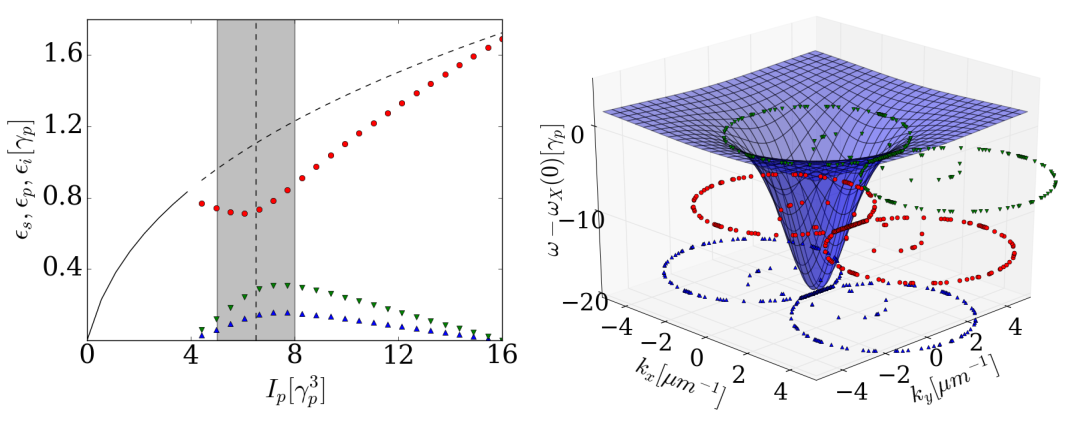
\includegraphics[width=.9\linewidth]{3d0_0} % ~/notebooks/OPODrag/opodrag.py
\caption{OPO mean-field blueshifts and fluctuation
  Rayleigh rings in the linear-response scheme for homogeneous
  pumping. Left panel: signal $s$ ([blue] upper triangles), pump $p$
  ([red] circles), and idler $i$ ([green] lower triangles) mean-field
  energy blueshifts $\epsilon_{n=s,p,i}$ (in units of $\gamma_p =
  \gamma_{\vt{k}_p}$) vs the rescaled pump intensity $I_p$ (in
  units of $\gamma_p^3$) in the optical limiter regime. Parameters are
  $\Omega_R=5$~meV, zero cavity-exciton detuning, $\gamma_X = \gamma_C
  = 0.12$~meV, $\omega_p - \omega_0^X = -1.25$~meV, $k_p=1.6{\mu
    m}^{-1}$, $k_s \simeq 0$, and $k_i=3.2{\mu m}^{-1}$.  The shaded
  area is stable OPO region, while the vertical dashed line
  corresponds to the pump power value chosen for plotting the right
  panel. Right panel: blueshifted LP dispersion~\eqref{eq:blues} with
  superimposed Rayleigh curves $\Gamma_{p,i,(u,v), \tilde{\vt{k}} +
    \vt{k}_{p, i}}$ evaluated within the linear-response
  approximation (same symbols as left panel). The two rings
  corresponding to the signal state, $\Gamma_{s,(u,v),
    \tilde{\vt{k}}}$, are shrunk to zero because $k_s \simeq 0$.}
\label{fig:spect}
\end{figure}
%


\section{Linear-response theory}
\label{sec:line-resp-theory}
In the limit where the homogeneously pumped system is only weakly
perturbed by the external potential $V_d(\vt{r})$, we apply a
linear-response analysis~\cite{Astrakharchik_2004}: The LP field is
expanded around the mean-field terms for the three $n=1,2,3=s,p,i$ OPO
states~\cite{Whittaker_2005} (see Eqs.~\eqref{eq:3-state-ansatz}
and~\eqref{eq:pump-fluctuations})
%
\begin{equation}
  \psi_{\tilde{\vt{k}}}^{} = \sum_{n=1}^3 e^{-i \omega_n t}
  \left[\psi_{n}^{} \delta_{\tilde{\vt{k}},0} +
    u_{n,\tilde{\vt{k}}}^{} e^{-i\omega t} +
    v^*_{n,-\tilde{\vt{k}}} e^{i\omega t} \right]\; ,
\label{eq:expan}
\end{equation}
%
where $\tilde{\vt{k}} = \vt{k} - \vt{k}_n$. Eq.~\eqref{eq:efflp} is
expanded linearly in both the fluctuation terms,
$u_{n,\tilde{\vt{k}}}^{}$ and $v_{n,\tilde{\vt{k}}}^{}$, as well as
the defect potential.  At zeroth order, the three complex uniform
mean-field equations can be solved to obtain the dependence of the
signal, pump and idler energy blueshifts,
$\epsilon_n = g_X X^2_{\vt{k}_n} |\psi_{n}^{}|^2$ on the system
parameters~\cite{Wouters_2007_b}. A typical behaviour of $\epsilon_n$
as a function of the rescaled pump intensity
$I_p = g_X C_{\vt{k}_p}^2 f_p^2/X_{\vt{k}_p}^2$ in the optical limiter
regime is plotted in the left panel of Fig.~\ref{fig:spect} (compare
to Fig.~\ref{fig:spi} of Sec.~\ref{sec:opo}).
%
At first order, one obtains six coupled equations diagonal in momentum
space~\cite{Wouters_2007}
%
\begin{equation}
  \omega \vt{w}_{\tilde{\vt{k}}} = \mathcal{L}_{\tilde{\vt{k}}}
  \vt{w}_{\tilde{\vt{k}}} + \frac{1}{2} \bm{\Psi}_d\; ,
\label{eq:fluct}
\end{equation}
%
for the six-component vector
$\vt{w}_{\tilde{\vt{k}}} = (u_{n,\tilde{\vt{k}}}^{} ,
v_{n,\tilde{\vt{k}}}^{})^{T}$ and for the potential part,
$\bm{\Psi}_d = (\psi_n^{} C_{\vt{k}_n} C_{\vt{k} + \vt{k}_n}
V_d(\vt{k}),-\psi_n^* C_{\vt{k}_n} C_{\vt{k}_n - \vt{k}}
V_d(-\vt{k}))^{T}$. To understand the origin of the factor $1/2$ in
Eq.~\eqref{eq:fluct}, it is sufficient to consider one component only,
and start from Eq.~\eqref{eq:mfield} used in Sec.~\ref{sec:linea}. The
connection becomes clear once we write the fluctuation part as
$\delta\psi(\rv,t) = \frac{1}{2}\left\{\delta\psi(\rv,t)
  +\left[\delta\psi^{\star}(\rv,t)\right]^{\star}\right\}$ and compare
it to Eq.~\eqref{eq:pump-fluctuations} of Sec.~\ref{sec:eq-state}.

In ~\eqref{eq:fluct} we have only kept the terms oscillating at the
frequencies $\omega_n \pm \omega$ and neglected the other terms in the
expansion (i.e., $2\omega_n - \omega_m \pm \omega$), which are
oscillating at frequencies far from the LP band, and thus with
negligible amplitudes.
%
In the particlelike and the holelike channels, the Bogoliubov matrix
determining the spectrum of excitations can be written
as~\cite{Wouters_2007}
%
\begin{equation}\label{eq:bogoliubov-opo}
  \mathcal{L}_{\vt{k}} = \begin{pmatrix} M_{\vt{k}}^{} & Q_{\vt{k}}^{}
    \\ -Q_{-\vt{k}}^* & -M_{-\vt{k}}^* \end{pmatrix} \; ,
\end{equation}
%
where the three OPO states components are
%
\begin{align}
  (M_{\vt{k}}^{})_{mn} &= \left[\omega^{LP}_{\vt{k}_m + \vt{k}}
    - \omega_m - i\frac{\gamma_{\vt{k}_m + \vt{k}}}{2}\right]
  \delta_{m,n} \\
%
  \nonumber & + 2\sum_{q,t=1}^3
  g_{\vt{k}_m+\vt{k},\vt{k}_n+\vt{k},\vt{k}_t} \psi_q^*
  \psi_t^{} \delta_{m+q,n+t}\\
%
  (Q_{\vt{k}}^{})_{mn} &= \sum_{q,t=1}^3
  g_{\vt{k}_m+\vt{k},\vt{k}_q,\vt{k}_t} \psi_q^{} \psi_t^{}
  \delta_{m+n,q+t}\; .
\end{align}
%
\begin{figure}[tb]
\centering
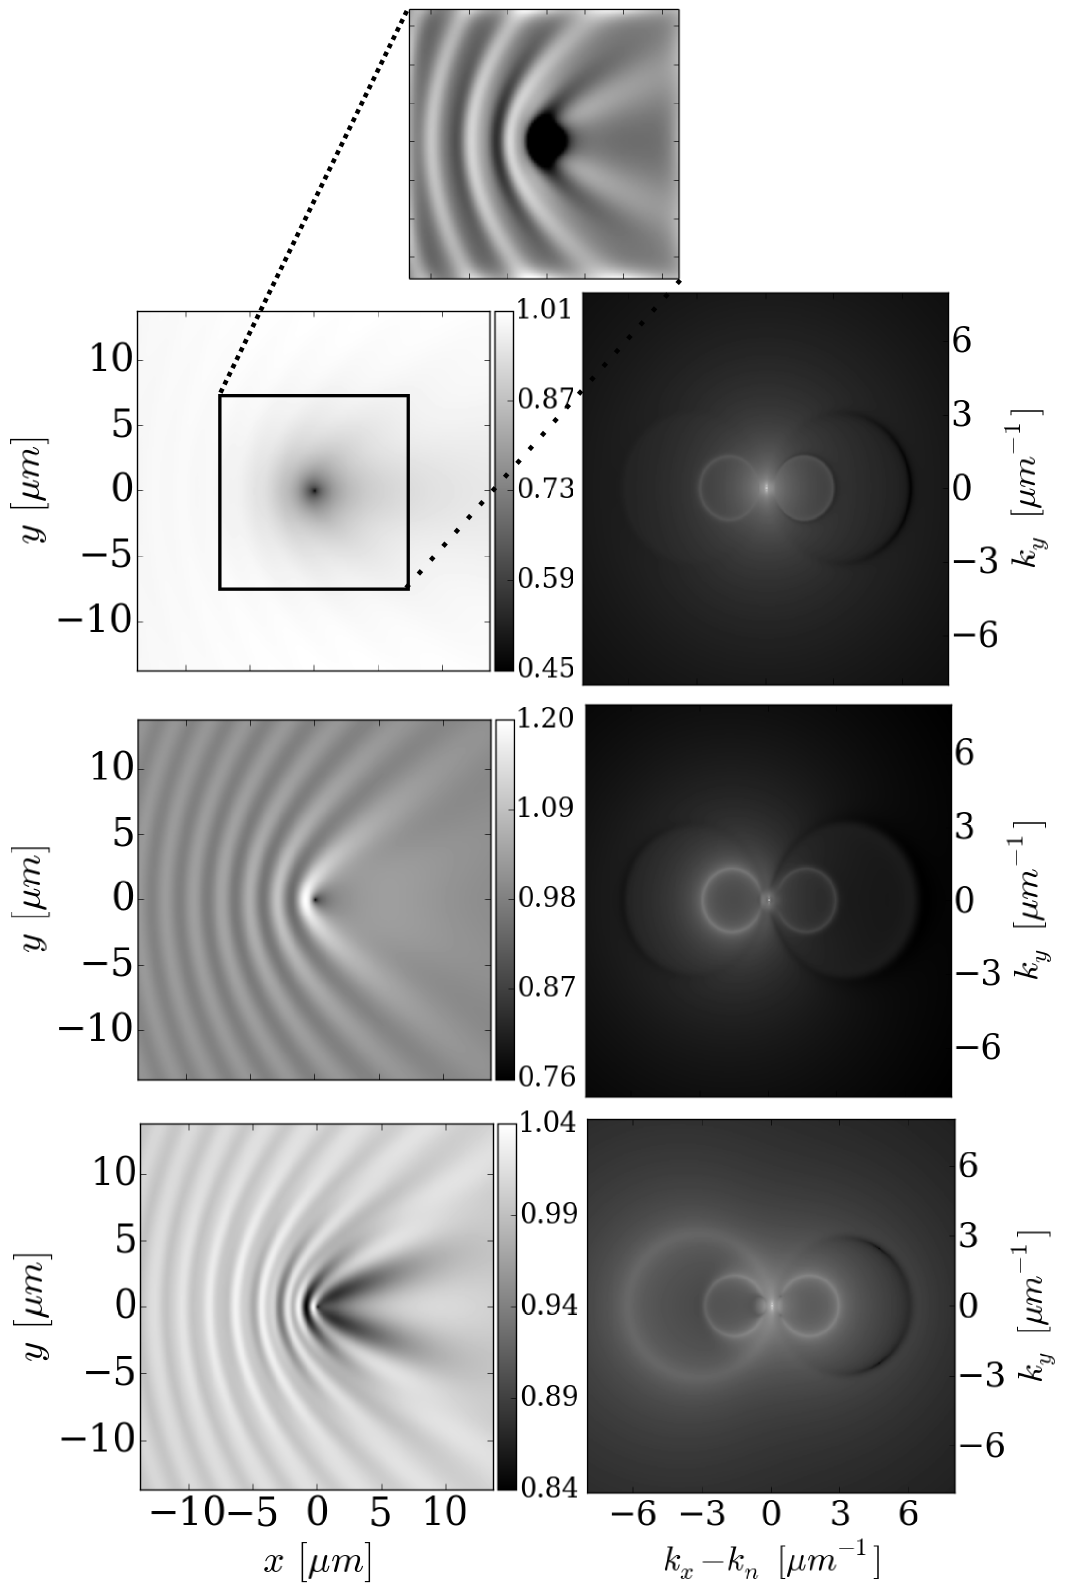
\includegraphics[width=.5\linewidth]{ks0_0}
% ~/notebooks/julia/april/linresp_waves.ipynb
% ~/notebooks/OPODrag/opodrag.py
\caption{Linear responses to a static defect of the three OPO states
  in real and momentum space. Rescaled filtered OPO emissions (signal
  [top panels], pump [middle], and idler [bottom]) in real space
  $|\psi (\vt{r},\omega_n)|^2/|\psi_n|^2$ (left panels in linear
  scale) and momentum space $|\psi_{\tilde{\vt{k}}} (\omega_n)|^2$
  (right panel in logarithmic scale) obtained within the
  linear-response approximation. The OPO parameters are the same ones
  in Fig.~\ref{fig:spect}, and the strength of the $\delta$-like
  defect potential, $V_d(\kv) = g_d$, is fixed to
  $g_d = 0.5 \gamma_p~\mu$m$^2$. For the top left panel of the signal
  emission in real space, Gaussian filtering is applied to enhance the
  short wavelength modulations, the amplitudes of which are otherwise
  roughly $1\%$ of the average signal intensity and about a factor of
  10 times weaker than the modulation amplitudes in the pump fluid.}
\label{fig:ereal}
\end{figure}
%

In absence of a defect potential ($\bm{\Psi}_d =0$),
Eq.~\eqref{eq:fluct} is the eigenvalue equation for the spectrum of
excitations of a homogeneous OPO, i.e.,
$\det(\mathcal{L}_{\tilde{\vt{k}}} - \omega)=0$. The spectrum has six
branches, $\omega_{n,(u,v),\tilde{\vt{k}}}$, labeled by $n=s,p,i$
and $(u,v)$. Even though these degrees of freedom are mixed together,
at large momenta, one recovers the LP dispersions shifted by the three
states' energies and momenta, i.e.,
%
\begin{equation}
  \lim_{\tilde{k} \gg \sqrt{2m_C \Omega_R}} \omega_{n,(u,v),\tilde{\vt{k}}} = \pm
  (\omega^{LP}_{\vt{k} - \vt{k}_n} - \omega_n)\; ,
\label{eq:large}
\end{equation}
%
where $+$ ($-$) corresponds to the $u$ ($v$) particlelike (holelike)
branch.
%
The OPO solution is stable (shaded area in Fig.~\ref{fig:spect}) as
far as $\Im[\omega_{n,(u,v),\tilde{\vt{k}}}] < 0$. Note also that,
owing to the $U(1)$ symmetry of the OPO equations of motion (see
Sec.~\ref{sec:opo}), no restoring force would oppose a rotation of the
signal-idler phases, meaning that the generator of such global
rotations,
$(i\psi_s,0,-i\psi_i,-i\psi_{s}^{\star},0,i\psi_{i}^{\star})$, is an
eigenvector of $\mathcal{L}_{\tilde{\vt{k}} = 0}$ with eigenvalue
$0$~\cite{Wouters_2007}.


The shape of the patterns, or Cherenkov-like waves, resulting from the
elastic scattering of the OPO 3-fluids against the static ($\omega=0$)
defect can be determined starting from the spectrum, and in particular
evaluating the closed curves $\Gamma_{n,(u,v), \tilde{\vt{k}}}$ in
$\vt{k}$-space, or ``Rayleigh rings''~\cite{9783319002651} defined by
the condition $\Re[\omega_{n,(u,v), \tilde{\vt{k}}}] = 0$. Even if
they do not appear to be relevant here, note that the presence of a
non-vanishing imaginary part of the excitation spectrum
$\Im[\omega_{n,(u,v),\tilde{\vt{k}}}]\neq 0$ introduces some
complications: Even in the absence of any Rayleigh ring, the drag
force can be non-vanishing and the standard Landau criterion may fail
to identify a critical velocity~\cite{Wouters_2010}.
%
The modulations propagate with a direction
$\hat{\eta}_{n,(u,v),\tilde{\vt{k}}}$ orthogonal to each curve
$\Gamma_{n,(u,v), \tilde{\vt{k}}}$, a pattern wavelength given by
the corresponding $|\tilde{\vt{k}}|$, and a group velocity
$\vt{v}_{n,(u,v),\tilde{\vt{k}}}^{(g)}=\nabla_{\tilde{\vt{k}}}
\Re[\omega_{n,(u,v), \tilde{\vt{k}}}]$, where
$\xi_{n,(u,v),\tilde{\vt{k}}} =
|\vt{v}_{n,(u,v),\tilde{\vt{k}}}^{(g)} / \Im[\omega_{n,(u,v),
  \tilde{\vt{k}}}]|$ determines the distance, at any given direction
$\hat{\eta}_{n,(u,v),\tilde{\vt{k}}}$, over which the perturbation
extends away from the defect. For a single fluid under a coherent
pump, the qualitative shape of the modulation pattern generated in the
fluid by the defect is mostly determined by the excitation
spectrum~\cite{Carusotto_2006,Carusotto_2004}.

For OPO, the spectrum of excitation on top of each of the three,
$n=1,2,3$, states (see appendix~\ref{app:SM}) generates six identical
Rayleigh rings $\Gamma_{n,(u,v), \tilde{\vt{k}}}$ for the three states.
%
The Rayleigh rings for the OPO conditions specified in
Fig.~\ref{fig:spect} are clearly visible in the right panels of
Fig.~\ref{fig:ereal}, where we plot the $\vt{k}$-space
photoluminescence filtered at the energy of each state, i.e.,
$|\psi_{\tilde{\vt{k}}} (\omega_n)|^2= |\psi_{n}^{}
\delta_{\tilde{\vt{k}},0} + u_{n,\tilde{\vt{k}}}^{} +
v^*_{n,-\tilde{\vt{k}}}|^2$.
%
We have chosen here a $\delta$-like defect potential, $V_d(\vt{k}) =
g_d$, but we have  checked that our results do not depend on
its exact shape (see appendix~\ref{app:SM}).
%
For the OPO conditions considered here, the signal momentum is at $k_s
\simeq 0$, and thus only four of the six rings are present. The same
rings are also plotted in the right panel of Fig.~\ref{fig:spect},
shifted at each of the three OPO states' momentum $\vt{k}_n$,
$\Gamma_{n,(u,v), \tilde{\vt{k}}+\vt{k}_n}$ and energies
$\omega_n$.
%
It is important to note that, even though the three OPO states have
locked responses because they display the same spectrum of
excitations, only one of the rings $\Gamma_{n,(u,v),
  \tilde{\vt{k}}+\vt{k}_n}$ is the most resonant at $\omega_n$
with the interaction blueshifted LP dispersion,
%
\begin{equation}
  \bar{\omega}_{\vt{k}}^{LP} = \omega_{\vt{k}}^{LP} + 2 
  X_{\vt{k}}^2 \sum_{n=1}^3  \epsilon_n\; ,
\label{eq:blues}
\end{equation}
%
where $\epsilon_n = g_X X_{\vt{k}_n}^2 |\psi_n^{}|^2$ are the
mean-field energy blueshifts (measured in Fig.~\ref{fig:spect} in
units of $\gamma_p = \gamma_{\vt{k}_p}$).  This implies that the
most visible modulation for each fluid should be the most resonant
one, with superimposed weaker modulations coming from the other two
state rings.

In the specific case of Fig.~\ref{fig:spect}, the signal is at $k_s
\simeq 0$ and thus produces no rings in momentum space. The other four
rings are very far from being resonant with the blueshifted LP
dispersion~\eqref{eq:blues} at $\omega_s$, and thus the signal
displays only an extremely weak modulation coming from the next
closer ring, which is the one associated with the pump state,
$\Gamma_{p,u, \tilde{\vt{k}}+\vt{k}_s}$.
%
We estimate that the signal modulation amplitudes are roughly $1\%$ of
the average signal intensity and about a factor of 10 times weaker
than the modulation amplitudes in the pump fluid.
%
To show that the signal has weak modulations coming from
the pump, we apply a Gaussian filter to the real space images (see the
inset of the top-left panel of Fig.~\ref{fig:ereal}).
%
As explained in more detail in appendix~\ref{app:SM}, Gaussian
filtering consists of subtracting from the original data a copy that
has been convoluted with a Gaussian kernel, thus getting rid of the
long-wavelength modulations.
%
This procedure reveals that indeed the pump imprints its modulations
also into the signal, even though these are extremely weak, thus
leaving the signal basically insensitive to the presence of the
defect.

Pump and idler states are each mostly resonant with their own
rings, i.e., $\Gamma_{p,u, \tilde{\vt{k}}+\vt{k}_p}$ at $\omega_p$
and $\Gamma_{i,u, \tilde{\vt{k}}+\vt{k}_i}$ at $\omega_i$,
respectively. Thus one should then observe two superimposed
modulations in both pump and idler filtered emissions, the stronger
one for each being the most resonant one.
%
However, the modulations associated with the idler only propagate very
close to the defect, at an average distance
$\overline{\xi_{i,u,\tilde{\vt{k}}}} \sim 1.7~\mu$m before getting
damped, and thus are not clearly visible. For the OPO conditions
considered, this is due to the small idler group velocity
$\vt{v}_{i,u,\tilde{\vt{k}}}^{(g)}$, as the dispersion is almost
excitonic at the idler energy.

We can conclude that, for the typical OPO condition with a signal at
$k_s \simeq 0$, considered in Figs.~\ref{fig:spect}
and~\ref{fig:ereal}, the signal fluid does not show modulations and
the extremely weak scattering inherited from the pump state can be
appreciated only after a Gaussian filtering procedure of the image. In
contrast, the idler has a locked response to the one of the pump
state.
%
Note that, for the conditions shown in Fig.~\ref{fig:spect}, as well
as the other cases considered in appendix~\ref{app:SM}, the subsonic to
supersonic crossover of the pump-only state~\cite{Amo_2009} happens
well above the region of stability of OPO. Thus it is not possible to
study a case where the pump is already subsonic and at the same time
promotes stimulated scattering.


\section{Experiments}
%
\begin{figure}[tb]\centering
  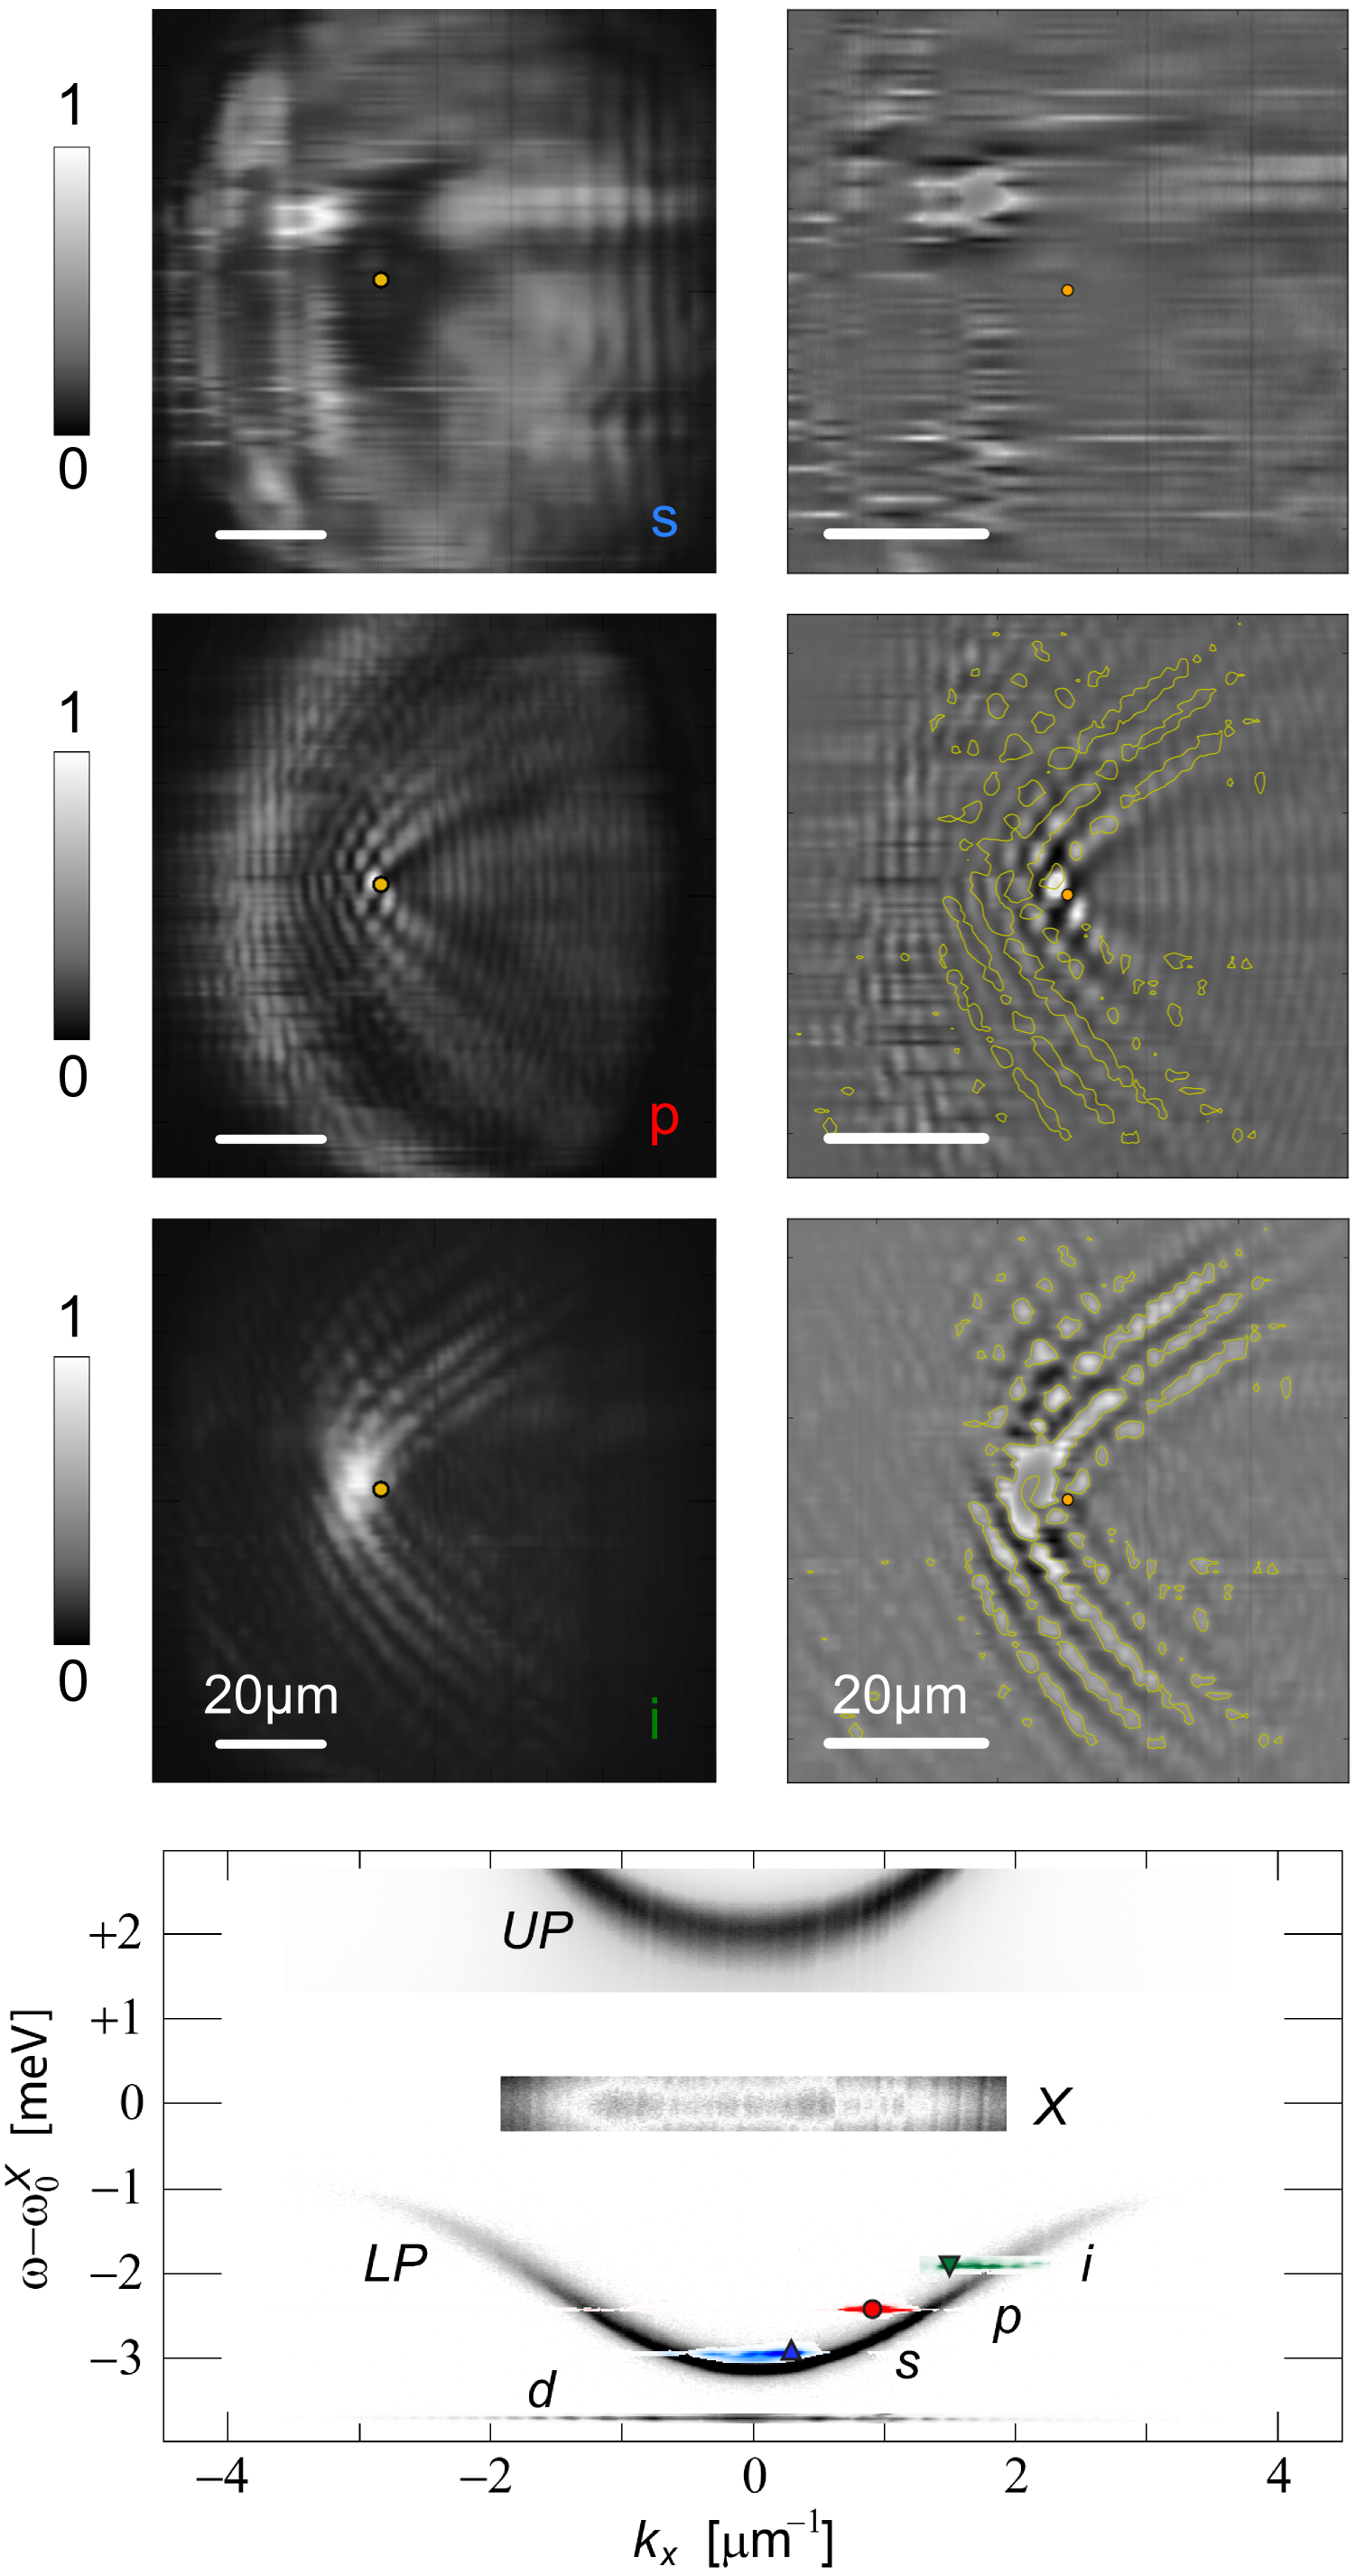
\includegraphics[width=.5\linewidth]{exp_waves}
  % ~/notebooks/julia/april/extract_exp_waves.ipynb
  \caption{Experimental OPO spectrum (lower panel) and filtered
    emissions of signal (top), pump (middle), and idler (bottom) in
    presence of a structural defect. The six panels show the filtered
    emission profiles in real space $I_{s, p,i}(\vt{r})$. A Gaussian
    filtering to enhance the short wavelength modulations is applied
    in the right column. The extracted wave crests from the idler
    (yellow contours in the bottom panel) are also superimposed on the
    pump profile (middle) by applying a $\pi$ phase-shift.}
\label{fig:exper}
\end{figure}
%
%
\begin{figure}[tb]
\centering
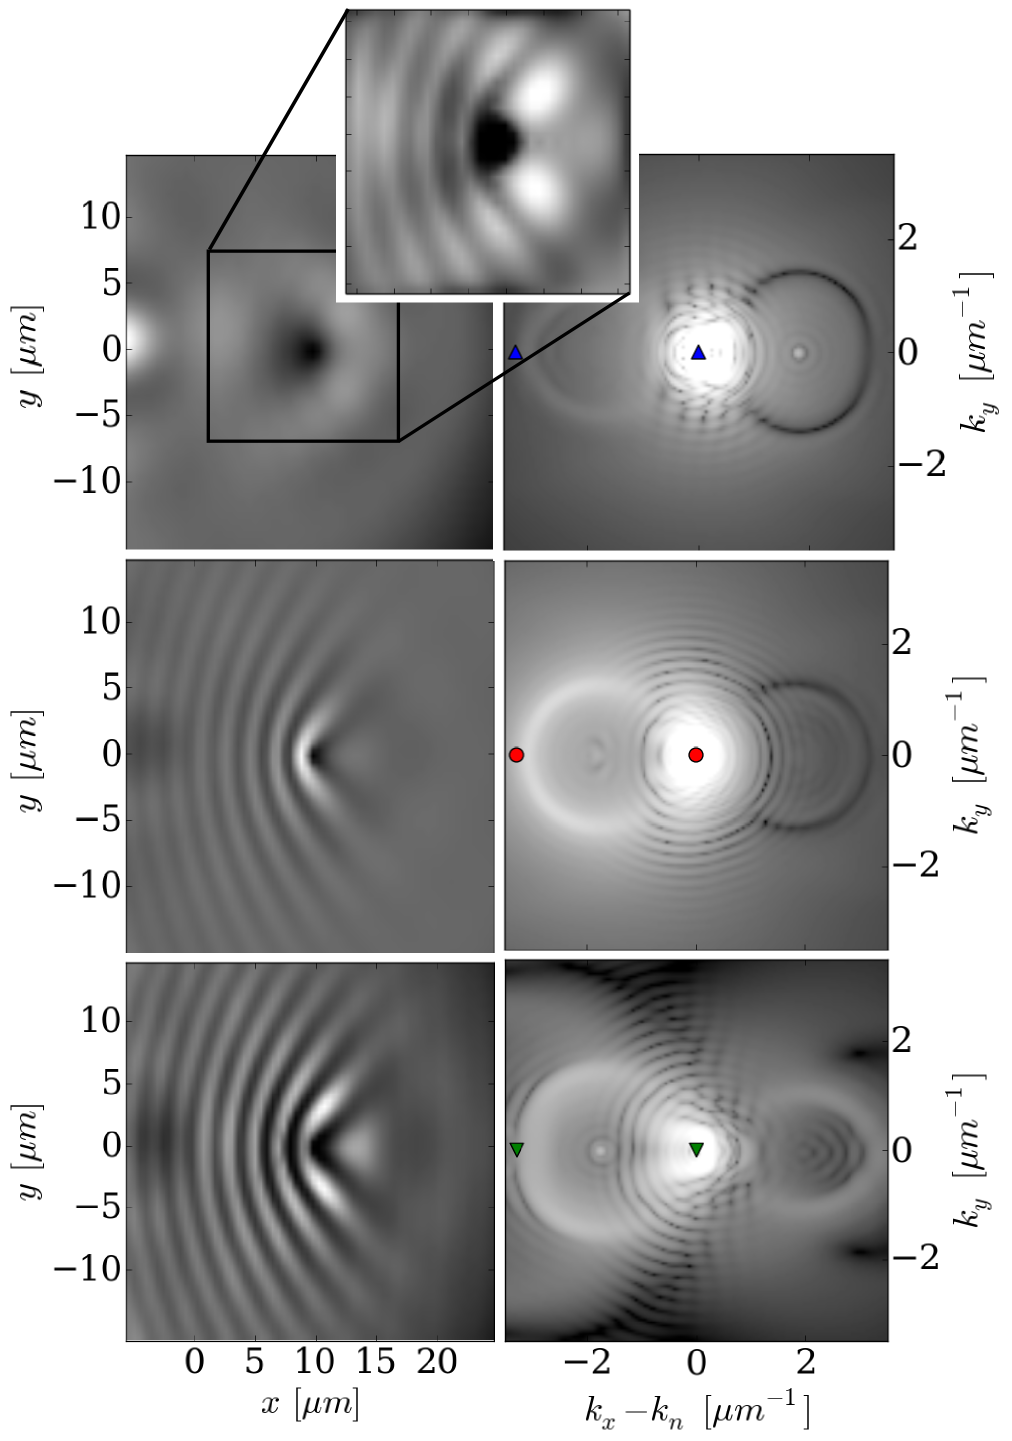
\includegraphics[width=.5\linewidth]{GP_space_mom}
% ~/Development/gp-linear-response/filtering-theory-GP.py
% ~/notebooks/julia/april/GP_signal_inset.ipynb
\caption{Full numerical responses to a static defect of
  the three OPO states in real and momentum space. Filtered OPO
  emissions (signal [top panels], pump [middle], and idler [bottom])
  in real space $|\psi_C (\vt{r},\omega_n)|^2$ (left panels in
  linear scale) and momentum space $|\psi_C
  (\tilde{\vt{k}},\omega_n)|^2$ (right panel in logarithmic scale)
  obtained by a full numerical evaluation of~\eqref{eq:gpequ}. For the
  top left panel of the signal space emission, Gaussian filtering is
  applied to enhance the short wavelength modulations of this state,
  revealing that the modulations corresponding to the pump state are
  also imprinted (though weakly) into the signal. The symbols indicate
  the pump ring diameter extracted from fitting the upstream
  modulations and resulting in a density-wave wavevector coinciding
  with that of the pump, $k_p=1.6$~$\mu$m$^{-1}$.}
\label{fig:numer}
\end{figure}
%
We now turn to the experimental analysis, where a continuous-wave
laser is used to drive a high quality ($Q=14000$) GaAs microcavity
sample into the OPO regime --- details on the sample can be found in
Refs.~\cite{Ballarini_2013,Dominici_2014}.
%%
The polariton dispersion is characterised by a Rabi splitting
$\Omega_R=5.4$~meV and the exciton energy is
$\omega_0^{X}=1485.26$~meV, while the cavity-exciton detuning is
slightly negative, $-1$~meV. The pump is at $k_p=0.89~\mu$m$^{-1}$ and
$\omega_p - \omega_0^{X}=-2.43$~meV, and, at pump powers $1.5$-times
above threshold, an OPO appears, with signal at small wavevector
$k_s=0.21~\mu$m$^{-1}$ and $\omega_s - \omega_0^{X}=-2.95$~meV, and
idler at $k_i=1.57~\mu$m$^{-1}$ and
$\omega_i - \omega_0^{X}=-1.91$~meV.
%
The defect used in the sample is a localized inhomogeneity naturally
present in the cavity mirror. Note that the exact location of the
defect can be extracted from the emission spectrum and is indicated
with a dot (orange) symbol in the profiles of Fig.~\ref{fig:exper}.

To filter the emission at the three states' energies,
$I_{s,p,i}(\vt{r}=x,y)$, and to obtain 2D spatial maps for the three
OPO states, one uses a spectrometer and, at a fixed position $x_0$,
one obtains the intensity emission as a function of energy and
position, $I(\epsilon,x_0,y)$. By changing $x_0$ one can build the
full emission spectrum as a function of energy and 2D position,
$I(\epsilon,\vt{r})$. The filtered emission for each OPO state is
obtained from the integrals
$I_{n=s,p,i}(\vt{r}) = \int_{\omega_n-\sigma}^{\omega_n+\sigma}
d\epsilon I(\epsilon, \vt{r})$, with $\sigma=0.08$~meV. The results
are shown in Fig.~\ref{fig:exper} for, respectively, the signal (top
panel), pump (middle) and the idler (bottom) profiles. Energy and
momentum of the three OPO states are labeled with a [blue] upper
triangle (signal), a [red] circle (pump), and a [green] lower triangle
(idler), while the localised state, clearly visible just below the
bottom of the LP dispersion, is indicated with the symbol $d$. The
bare LP dispersion is extracted from an off-resonant low pump power
measurement, as well as the emission of the exciton reservoir (X) and
that of the UP dispersion (each in a different scale).
%
The signal profile shows no appreciable modulations around the defect
locations, nor could any  be observed after applying a Gaussian
filtering procedure of the image.
%
In contrast, in agreement with the theoretical results, both filtered
profiles of the pump and idler show the same Cherenkov-like pattern. We
extracted the wave crests from the idler profile ([yellow] contours in
the bottom panel) and superimposed them on the pump profile (middle
panel) with an added $\pi$ phase-shift, revealing that the only
modulations visible in the idler state are the ones coming from the
pump state.


\section{Numerical analysis}
\label{sec:numerical-analysis}
%
The agreement between the results obtained experimentally and within
the linear-response approximation is additionally confirmed by an
exact full numerical analysis of the coupled
equations~\eqref{eq:gpequ} for a finite size pump via a
5$^{\text{th}}$-order adaptive-step Runge-Kutta algorithm.
%
Details are given in appendix~\ref{app:SM}.
%
The pumping conditions are very similar to those previously considered
in the linear-response approximation of Figs.~\ref{fig:spect}
and~\ref{fig:ereal}, while the pump profile $\mathcal{F}_p(\vt{r})$ is
now a finite-size top hat. In particular, we consider the case of zero
cavity-exciton detuning, $k_p=1.6$~$\mu$m$^{-1}$,
$\omega_p-\omega_X^0 = -0.44$~meV and the pump power strength is fixed
just above threshold, such as to produce a stable steady state OPO.
This, in absence of the defect, is characterized by a signal at small
wavevector $k_s=-0.2$~$\mu$m$^{-1}$ and idler at
$k_i=3.4$~$\mu$m$^{-1}$.

When adding a localised defect potential, the steady state OPO
develops Rayleigh rings in momentum space, yet, as shown in appendix~\ref{app:SM},
the spectrum continues to be $\delta$-like in energy, allowing us to
easily filter in energy the emission of the three OPO states.
%
Results are shown in Fig.~\ref{fig:numer}, where real-space emissions
$|\psi_C (\vt{r},\omega_n)|^2$ are plotted in the left panels, while
the ones in momentum space $|\psi_C (\tilde{\vt{k}},\omega_n)|^2$ are
plotted in the right panels. We observe a very similar phenomenology
to that one obtained in the linear approximation shown in
Fig.~\ref{fig:ereal}. The signal now is at slightly negative values of
momenta $k_s=-0.2$~$\mu$m$^{-1}$, thus implying a very small Rayleigh
ring associated with this state. Thus we observe that only the
modulations associated with the pump are the ones that are weakly
imprinted in the signal state and that can be observed by means of a
Gaussian filtering (inset of the top-left panel). We have fitted the
upstream wave crests and obtained the same modulation wavevector as
the pump one ([blue] upper triangles). Similar to the linear-response
case, we also find here that the most visible perturbation in the
emission filtered at the idler energy is the one due to the pump
Rayleigh ring. As before, the modulations due to the idler Rayleigh
ring cannot propagate far from the defect because of the small group
velocity associated with this state.


\section{Conclusions}
%
To conclude, we have presented a joint theoretical and experimental
study of the superfluid properties of a nonequilibrium condensate of
polaritons in the so-called optical parametric oscillator
configuration by studying the scattering against a static defect.
%
We have found that, while the signal is basically free from
modulations, the pump and idler lock to the same response. We have
highlighted the role of the coupling between the OPO components due to
nonlinear and parametric processes. These are responsible for the
transfer of the spatial modulations from one component to the
other. This process is most visible in the clear spatial modulation
pattern that is induced by the nonsuperfluid pump onto the idler,
while the same modulations are only extremely weakly transferred into
the signal, because of its low characteristic wavevector, so much that
experimentally cannot be resolved.
%
The main features of the real- and momentum-space emission patterns
are understood in terms of Rayleigh scattering rings for each
component and a characteristic propagation length from the defect; the
rings are then transferred to the other components by nonlinear and
parametric processes.

Much interest has been recently devoted to aspects related to
algebraic order~\cite{Altman_2015,PhysRevX.5.041028} and superfluid
response~\cite{Keeling_2011_prl} in drive-dissipative polariton
condensates. Our theoretical and experimental results further stress
the complexities and richness involved when looking for superfluid
behavior in nonequilibrium multicomponent condensates such as the ones
obtained in the OPO regime.


\begin{subappendices}
\section{Signal state at nonzero momenta}
\label{app:SM}
%
\begin{figure}[tb]\centering
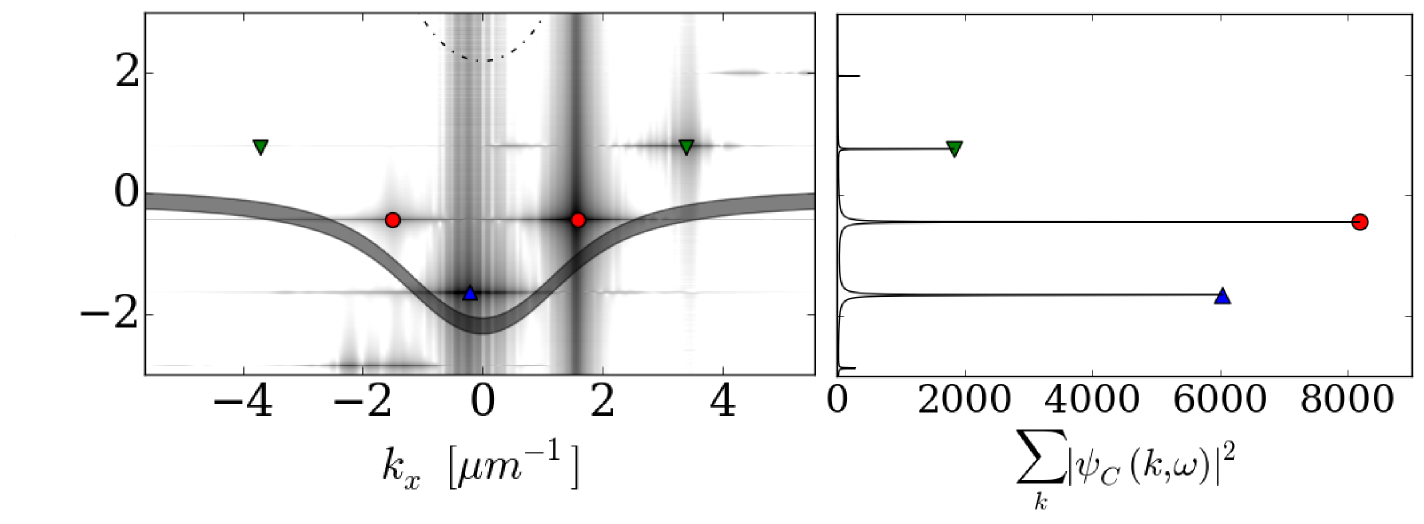
\includegraphics[width=.9\linewidth]{GP_disp}
% ~/notebooks/julia/theory-GP.ipynb
\caption{OPO spectrum obtained by full numerics. Left
  panel: Photonic component of the OPO spectrum in presence of a
  point-like defect, $|\psi_C(k_x,0,\omega)|^2$ (logarithmic scale),
  as a function of the rescaled energy $\omega - \omega_0^X$ versus
  the $x$-component of momentum $k_x$ (cut at $k_y=0$) for a top-hat
  pump (see text for the space profile and parameter values), with
  intensity $f_p=1.23 f_p^{\text{th}}$ above the OPO threshold, pump
  wave-vector $k_p=1.6$~$\mu$m$^{-1}$ in the $x$-direction and
  $\omega_p-\omega_X^0=-0.44$~meV. The symbols indicate the signal
  ([blue] upper triangle), pump ([red] circle), and idler ([green]
  lower triangle) energies, as well as the two momenta $k_x$ on each
  state Rayleigh ring at $k_y=0$. Note that the logarithmic scale
  results in a fictitious broadening in energy of the spectrum, which
  is in reality $\delta$-like (see right panel). The bare LP
  dispersion, including its broadening due to finite lifetime, is
  plotted as a shaded grey region, while the bare UP dispersion as a
  (black) dot-dashed line. Right panel: Momentum integrated spectrum,
  $\sum_{\vt{k}} |\psi_C(\vt{k},\omega)|^2$ (linear scale) as a
  function of the rescaled energy $\omega - \omega_0^X$, where it can
  be clearly appreciated that the emission is $\delta$-like in
  energy.}
\label{fig:spectGP}
\end{figure}
%
In Chapter~\ref{cha:opo}, we presented a theoretical and experimental
analysis of the response of microcavity polaritons in the OPO regime
to a static defect.
%
For the theoretical calculations we follow two independent approaches:
In the first approach, we exactly numerically solve the dynamics of
the two coupled Gross-Pitaevskii equations (GPEs) for the exciton and
cavity fields for the realistic case of a finite-size top-hat pump
profile $\mathcal{F}_p(\vt{r})$. In the second approach, we apply a
perturbative linear-response approximation for the LP
LP state, which leads to semi-analytical results in the limiting case
of a spatially homogeneous pump profile. Both methods have been
already successfully used in the literature to explore several
properties of the OPO operation.

While all fundamental formulae and information has been given in the
Chapter text, in this appendix we present some additional details on
both approaches that might be of interest to the specialized reader.
In addition to that, we make use of the linear-response approach to
examine some regimes that are hardly accessed experimentally or within
a full numerical approach.


\subsection{Full numerics}
\label{subsec:detun}
The classical driven-dissipative non-linear Gross-Pitaevskii equation
(GPE) for the coupled exciton and cavity fields
$\psi_{X,C} (\vt{r},t)$ (as given in Sec.~\ref{sec:model-opo})
%
\begin{equation}
  i\partial_t \begin{pmatrix} \psi_X \\ \psi_C \end{pmatrix} =
  \hat{H} \begin{pmatrix} \psi_X \\ \psi_C \end{pmatrix}
  + \begin{pmatrix} 0 \\ F_p(\vt{r},t) \end{pmatrix}\; ,
\label{eq:numer}
\end{equation}
%
where
%
\begin{equation}
  \hat{H} = \begin{pmatrix} \omega^{X}(-i\nabla) - i
    \frac{\gamma_X}{2} + g_X |\psi_X|^2 & \Omega_R/2 \\ \Omega_R/2 &
    \omega^C(-i\nabla) - i \frac{\gamma_C}{2} + V_d \end{pmatrix} \;
  ,
\end{equation}
%
is solved numerically on a 2D grid of $N\times N=2^8\times 2^8$ points
and a separation of $0.47$~$\mu$m (i.e., in a box $L\times L =
121$~$\mu$m$\times 121$~$\mu$m) by using a 5$^{\text{th}}$-order
adaptive-step Runge-Kutta algorithm. Convergence has been checked both
with respect the resolution in space $L/N$ as well as in momentum
$\pi/L$, without~\cite{Marchetti_2010,9783642241857} as well as in
presence of the defect.
%
The same approach has been already used in the literature, for a
review, see Refs.~\cite{Marchetti_2010,9783642241857}).
%
As for the system parameters, we have considered a LP dispersion at
zero photon-exciton detuning, $\omega^C_0 = \omega^X_0$, a
dispersionless excitonic spectrum, $\omega^X_{\vt{k}} = \omega^X_0$
and a quadratic dispersion for photons $\omega^C_{\vt{k}} =
\omega^C_0 + k^2/2m_C$, with the photon mass $m_C=2.3 \times 10^{-5}
m_e$, where $m_e$ is the bare electron mass. The LP dispersion, $2
\omega_{\vt{k}}^{LP} = \omega_{\vt{k}}^{C} + \omega_{\vt{k}}^{X}
- \sqrt{(\omega_{\vt{k}}^{C} - \omega_{\vt{k}}^{X})^2 +
  \Omega_R^2}$ is characterised by a Rabi splitting $\Omega_R =
4.4$~meV. Furthermore, the exciton and cavity decay rates are fixed to
$\gamma_X=\gamma_C=0.53$~meV.
%
For the defect we choose a $\delta$-like potential
%
\begin{equation}
  V_d(\vt{r}) = g_d \delta(\vt{r} - \vt{r}_0)\; ,
\end{equation}
%
where its location $\vt{r}_0$ is fixed at one of the $N \times N$
points of the grid.
%
Note that in a finite-size OPO, local currents lead to inhomogeneous
OPO profiles inside the pump spot, despite the external pump having
a top-hat profile with a completely flat inner
region~\cite{Marchetti_2010,9783642241857} --- as shown later, this
can be observed in the filtered OPO profiles evaluated in absence of a
defect, shown as dashed lines in Fig.~\ref{fig:rafull}.
%
We have thus chosen the defect location so that it lies in the
smoothest and most homogeneous part of the OPO profiles.
%
\begin{figure}[tb]\centering
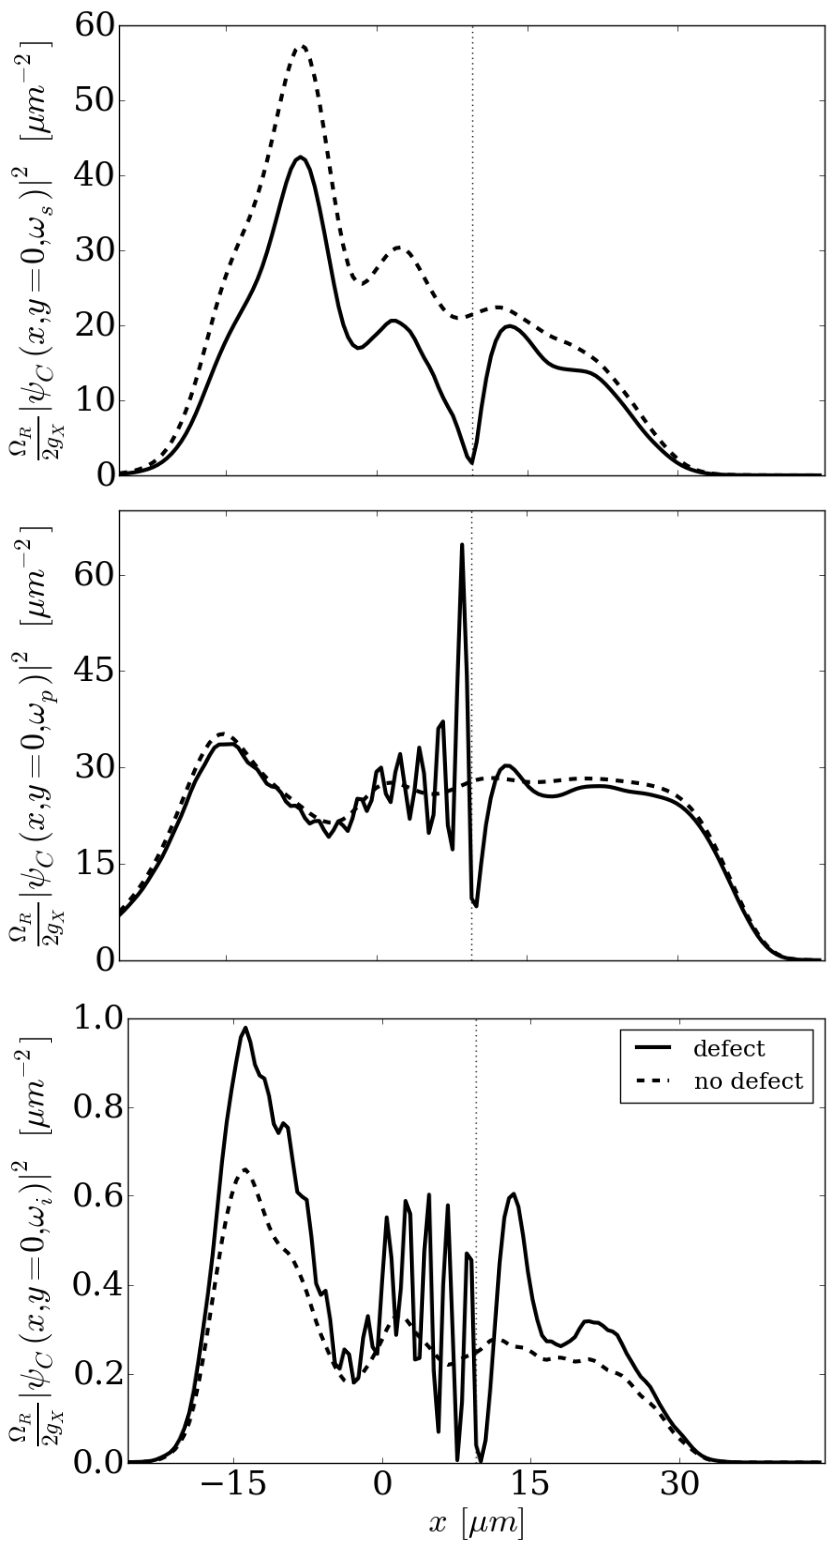
\includegraphics[width=.5\linewidth]{rangesGP.png}
% ~/Development/gp-linear-response/filtering-theory-GP.py
\caption{Real space signal, pump and idler OPO one-dimensional
  filtered profiles derived from finite size numerics with and without
  a defect. Rescaled OPO filtered emissions along the $y=0$ direction,
  $|\psi_C(x,y=0,\omega_n)|^2 \frac{\Omega_R}{2g_X}$, obtained by
  numerically solving the GPE Eq.~\eqref{eq:gpequ} of
  Sec.~\ref{sec:model-opo}. While the dashed lines represent the
  filtered emissions of signal (top panel), pump (middle) and idler
  (bottom) for a top-hat pump without a defect, the solid lines are
  the same OPO conditions but now for a defect positioned at
  $(x_d, y_d) = (9.5, -0.5)$~$\mu$m corresponding to the vertical
  dotted lines. The system parameters are the same ones as those of
  Fig.~\ref{fig:numer}.}
\label{fig:rafull}
\end{figure}
%

Also we have checked that our results do not qualitatively depend on
the strength $g_d$ (nor on the sign) of the defect potential, as far
as this does not exceed a critical value above which it destabilises
the OPO steady-state regime.
%
The pump, $F_p(\vt{r},t) = \mathcal{F}_p(\vt{r}) e^{i (\vt{k}_p
  \cdot \vt{r} - \omega_p t)}$, has a smoothen and rotationally
symmetric top-hat profile, $\mathcal{F}_p(\vt{r}) = \mathcal{F}_p(r)
= \frac{f_p}{2}[\tanh(\frac{r+\sigma_p}{r_0}) -
  \tanh(\frac{r-\sigma_p}{r_0})]$ with strength $f_p = 1.23
f_p^\text{th} = 0.053$~meV/$\mu$m and parameters $r_0 = 8.68~\mu$m,
$\sigma_p = 34.72~\mu$m.
%
We pump at $k_p=1.6$~$\mu$m$^{-1}$ in the $x$-direction, $\vt{k}_p =
(k_p,0)$, and at $\omega_p-\omega_X^0=-0.44$~meV, i.e., roughly
$0.5$~meV above the bare LP dispersion. By increasing the pump
strength $f_p$, we find the threshold $f_p^{\text{th}}$ above which
OPO switches on, leading to two conjugate signal and idler states.
%
We then fix the pump strength just above this threshold ($f_p=1.23
f_p^{\text{th}}$), where we find a steady state OPO solution which is
stable (see Ref.~\cite{9783642241857} for further details). In
absence of the defect, this condition corresponds to a signal state at
$k_s=-0.2$~$\mu$m$^{-1}$ and $\omega_s-\omega_0^X = -1.64$~meV and an
idler at $k_i=3.4$~$\mu$m$^{-1}$ and $\omega_i-\omega_0^X =
0.76$~meV. 
%
It is interesting to note that already very close to the lower pump
power threshold for OPO, the selected signal momentum is very close to
zero. This contrasts with what one obtains in the linear approximation
scheme, where instead just above the lower OPO threshold there exists
a broad interval of permitted values for $k_s$ (and thus $k_i$) --- we
will further discuss this ``selection problem'' for parametric
scattering in Sec.~\ref{subsec:analy}.

We evaluate the time dependent full numerical solution
of~\eqref{eq:numer} $\psi_{X,C} (\vt{r},t)$, until a steady state
regime is reached. Here, both its Fourier transform to momentum
$\vt{k}$ and energies $\omega$ can be evaluated numerically.
%
We plot on the left panel of Fig.~\ref{fig:spectGP} a cut at $k_y=0$
of the photonic component of the OPO spectrum in presence of a
point-like defect, $|\psi_C(k_x,0,\omega)|^2$, as a function of the
rescaled energy $\omega - \omega_0^X$ versus the $x$-component of
momentum $k_x$ (cut at $k_y=0$). In the right panel we plot instead
the corresponding momentum integrated spectrum, $\sum_{\vt{k}}
|\psi_C(\vt{k},\omega)|^2$.
%
Here, we can clearly see that the presence of the defect does not
modify the fact that the OPO emission for the OPO signal ([blue] upper
triangle), pump ([red] circle), and idler ([green] lower triangle)
states has a completely flat dispersion in energy, thus indicating
that a stable steady state OPO solution has been reached. Note that in
the spectrum map of the left panel of Fig.~\ref{fig:spect}, the
logarithmic scale results in a fictitious broadening in
energy. However, from the integrated spectrum plotted in linear scale
in the right panel of Fig.~\ref{fig:spect} one can clearly appreciate
that this emission is $\delta$-like, exactly as it happens for the
homogeneous OPO case~\cite{9783642241857}.
%
Thus the effect of the defect is to induce only elastic (i.e., at the
same energy) scattering; now the three OPO states emit each on its own
Rayleigh ring (given each by the symbols on the left panel of
Fig.~\ref{fig:spectGP} which represent the rings at a cut for
$k_y=0$). This makes it rather difficult to extract the separated
signal, pump and idler profiles by filtering in momentum, as done
previously for the homogeneous case, but it still allows to filter
those profiles very efficiently in energy. In fact, because the
emission is $\delta$-like, it is enough to fix a single value of the
energy $\omega$ to the one of the three states $\omega_{n=s,p,i}$,
thus extracting the filtered profiles either in real space
$|\psi_C(\vt{r},\omega_n)|^2$ or in momentum space
$|\psi_C(\vt{k},\omega_n)|^2$ --- we have however checked that
integrating in a narrow energy window around $\omega_n$ does not
quantitatively change the results.

The results of the above described filtering are shown in
Fig.~\ref{fig:numer}.
%
In Fig.~\ref{fig:rafull} we instead plot the corresponding
one-dimensional profiles in the $y=0$ direction both in presence
(solid line) and without (dashed line) a defect. Here, we can observe
that, even if the pump has a top-hat flat profile, as also commented
previously, in absence of a defect, the finite-size OPO is
characterised by inhomogeneous profiles of signal, pump and idler
because of localised currents. Further, we observe that the presence
of a defect induces strong modulations in pump and idler.
%
In order to reveal that the pump also imprints its modulation into the
signal, even though these are extremely weak (and hardly visible in
both the top main panel of Fig.~\ref{fig:numer} and the top panel of
Fig.~\ref{fig:rafull}), we apply a Gaussian filtering to the signal
images, the result of which is shown in the inset of the top-left
panel of Fig.~\ref{fig:numer}.
%
This consists of the following procedure. The original data for the
real space profile $\psi(\vt{r})$ are convoluted with a Gaussian
kernel $K(\vt{r} - \vt{r}')$, obtaining a new profile,
$\tilde{\psi}(\vt{r}') = \int d\vt{r} \psi (\vt{r}) K(\vt{r} -
\vt{r}')$, where short wavelengths features are smoothened out. The
convoluted image $\tilde{\psi}(\vt{r}')$ is then subtracted from the
original data, giving $\psi(\vt{r}) - \tilde{\psi}(\vt{r})$, and
effectively filtering out all long wavelength details.
%
The same procedure of Gaussian filtering is also applied to the signal
emission profile obtained within the linear-response analysis and
shown in the inset of the top left panel of Fig.~\ref{fig:ereal}.

%
\begin{figure}[tb]\centering
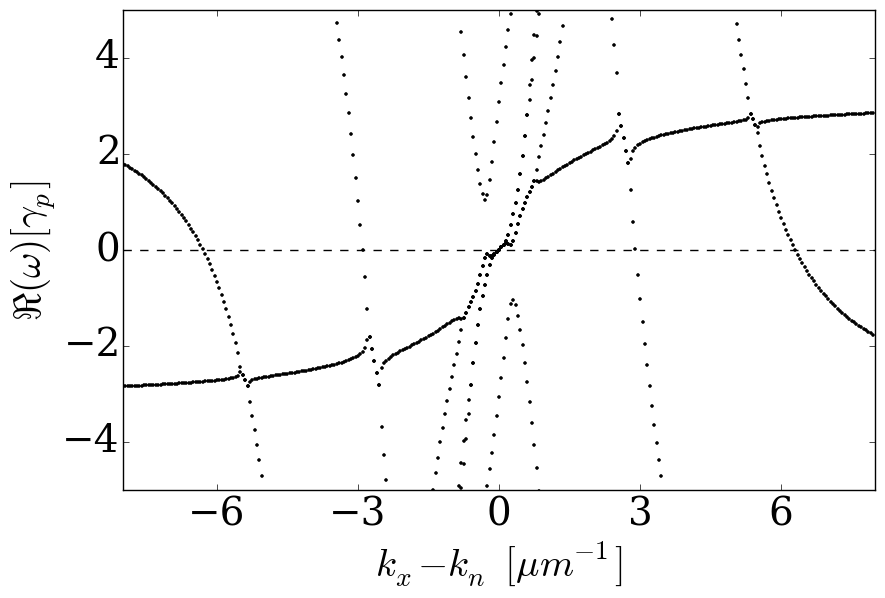
\includegraphics[width=.7\linewidth]{fig_excitation_ks_0_000.png}
% ~/notebooks/OPODrag/opodrag.py
\caption{Spectrum of collective excitations. Cut at $k_y=0$ of the
  real part of the quasiparticle energy dispersion
  $\Re [\omega_{n,(u,v),\vt{k}-\vt{k}_n}]$ plotted versus $k_x -
  k_n$. The spectrum is evaluated within the linear approximation
  scheme and the parameters are the same ones used for
  Fig.~\ref{fig:ereal}.}
\label{fig:bogol}
\end{figure}
%
%
\begin{figure}[tb]
\centering
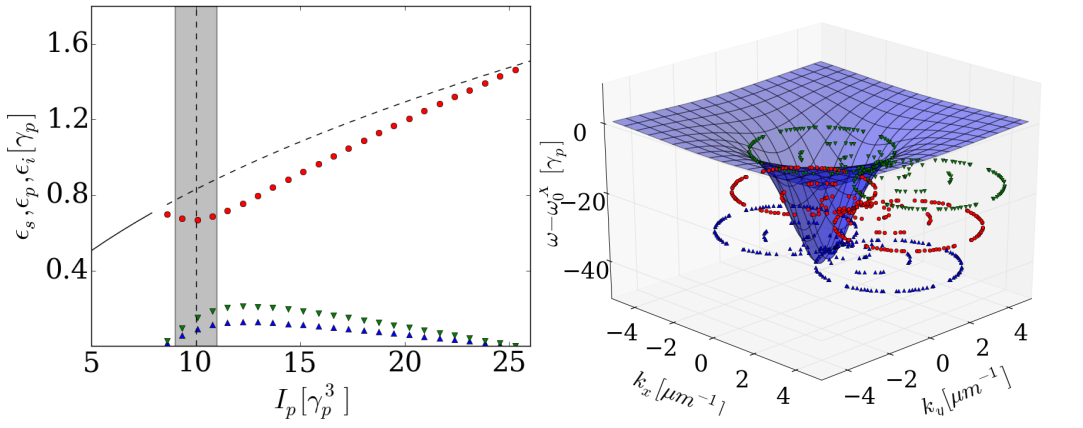
\includegraphics[width=.5\linewidth]{3d0_7.png}
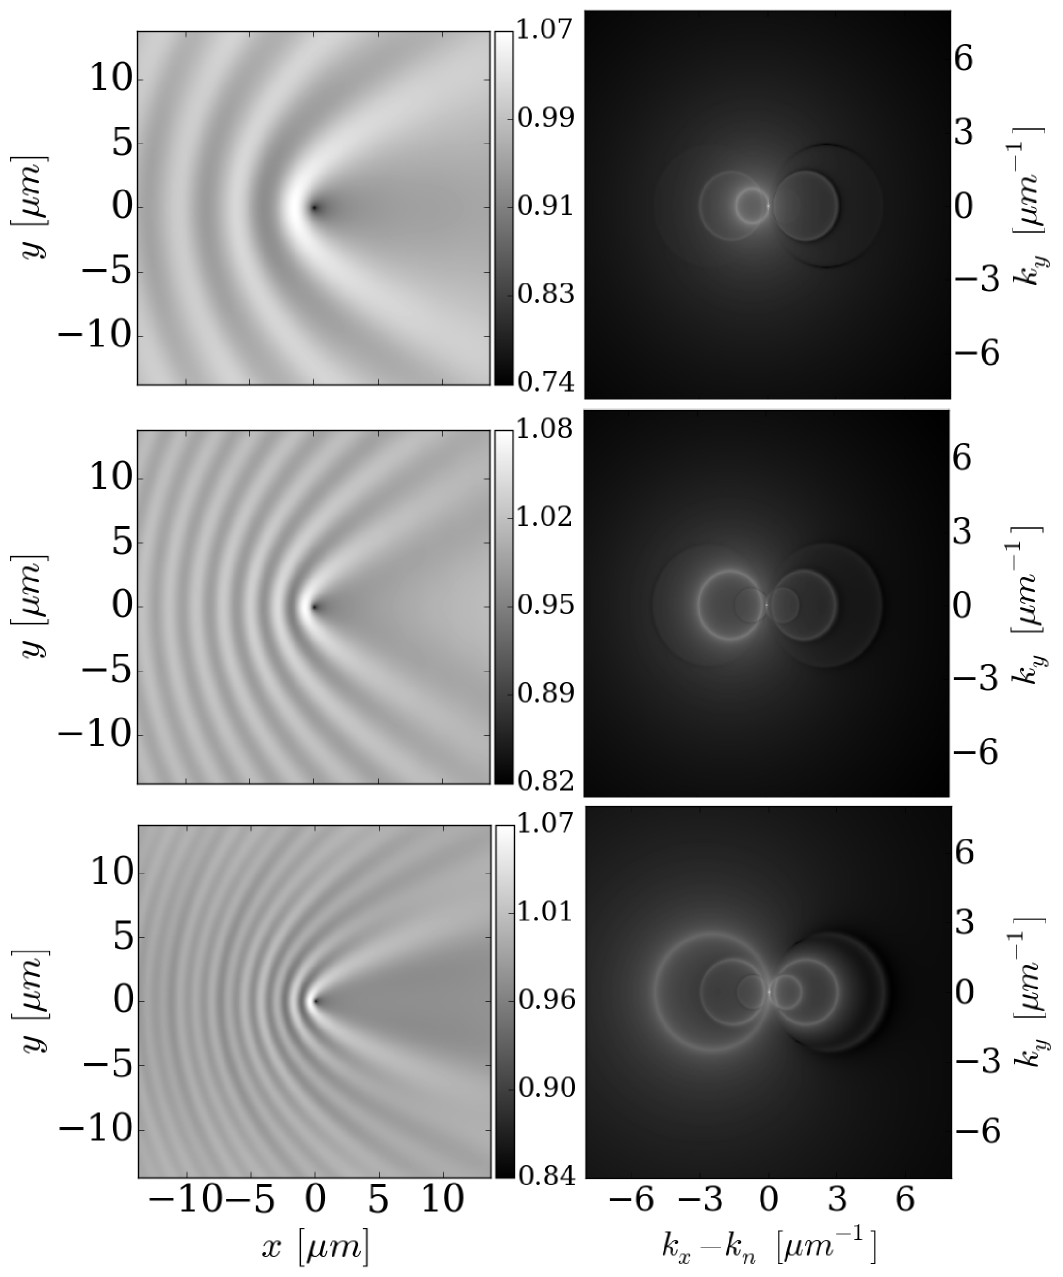
\includegraphics[width=.5\linewidth]{ks0_7.png}
% ~/notebooks/OPODrag/opodrag.py
\caption{OPO for finite and positive signal momentum in the
  linear-response approximation for homogeneous pumping. Rescaled OPO
  emission within the linear-response approximation in real
  $|\psi (\vt{r},\omega_n)|^2/|\psi_n|^2$ (left panels in linear
  scale) and momentum space $|\psi_{\tilde{\vt{k}}} (\omega_n)|^2$
  (right panels in linear scale) filtered at the energies of the three
  OPO states: signal (top panels), pump (middle), and idler
  (bottom). The parameters are the same as those used in
  Fig.~\ref{fig:ereal}, with the exception of the signal and idler
  momenta, which are now at $k_s = 0.7$~$\mu$m$^{-1}$ and
  $k_i = 2.5$~$\mu$m$^{-1}$ respectively. Each scale of variation for
  the profiles is plotted in the color-box next to the left panels. A
  cut in the $y=0$ direction for the three profiles is plotted in the
  bottom panel of Fig.~\ref{fig:range}.}
\label{fig:ksp07}
\end{figure}
%
%
\begin{figure}[tb]
\centering
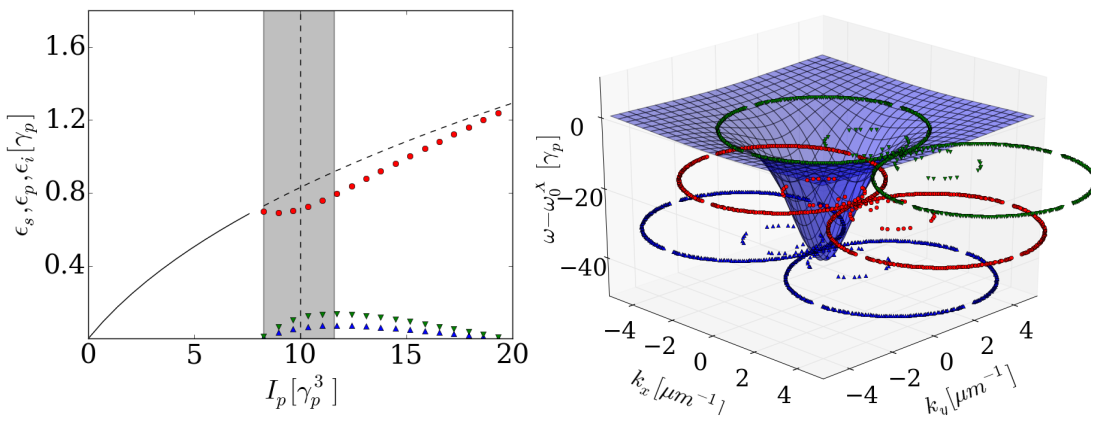
\includegraphics[width=.5\linewidth]{3d-0_4.png}
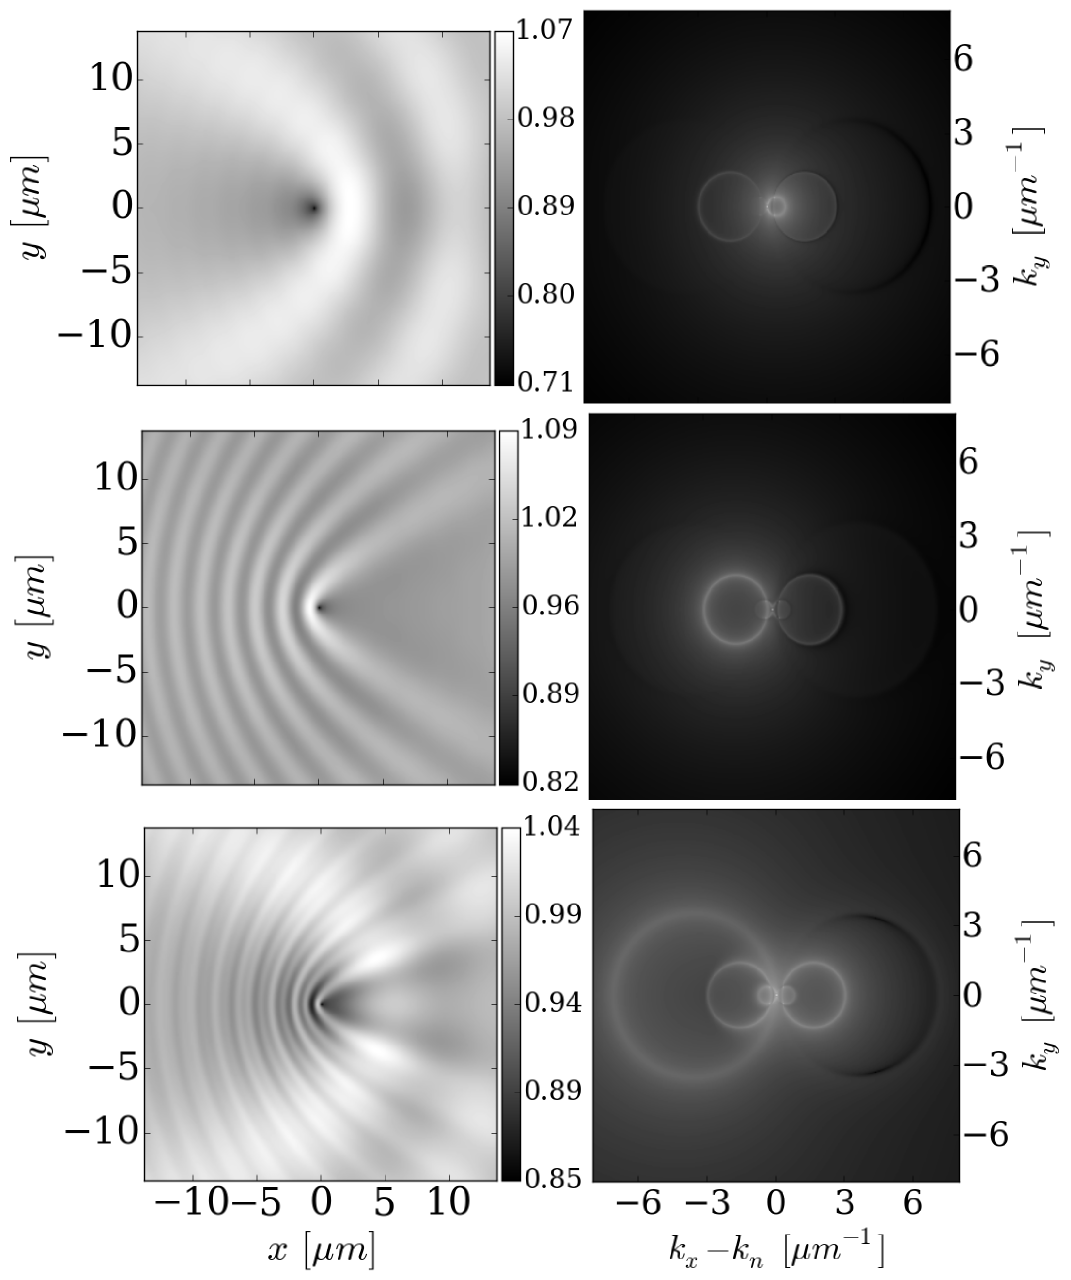
\includegraphics[width=.5\linewidth]{ks-0_4.png}
% ~/notebooks/OPODrag/opodrag.py
\caption{OPO for finite and negative signal momentum in the
  linear-response approximation for homogeneous pumping. Rescaled OPO
  emission within the linear-response approximation in real
  $|\psi (\vt{r},\omega_n)|^2/|\psi_n|^2$ (left panels in linear
  scale) and momentum space $|\psi_{\tilde{\vt{k}}} (\omega_n)|^2$
  (right panels in linear scale) filtered at the energies of the three
  OPO states: signal (top panels), pump (middle), and idler
  (bottom). The parameters are the same as those used in
  Fig.~\ref{fig:ereal}, with the exception of the signal and idler
  momenta, which are now at $k_s = -0.4$~$\mu$m$^{-1}$ and
  $k_i = 3.6$~$\mu$m$^{-1}$ respectively. A cut in the $y=0$ direction
  for the three profiles is plotted in the top panel of
  Fig.~\ref{fig:range}.}
\label{fig:ksm04}
\end{figure}
%
\begin{figure}[tb]\centering
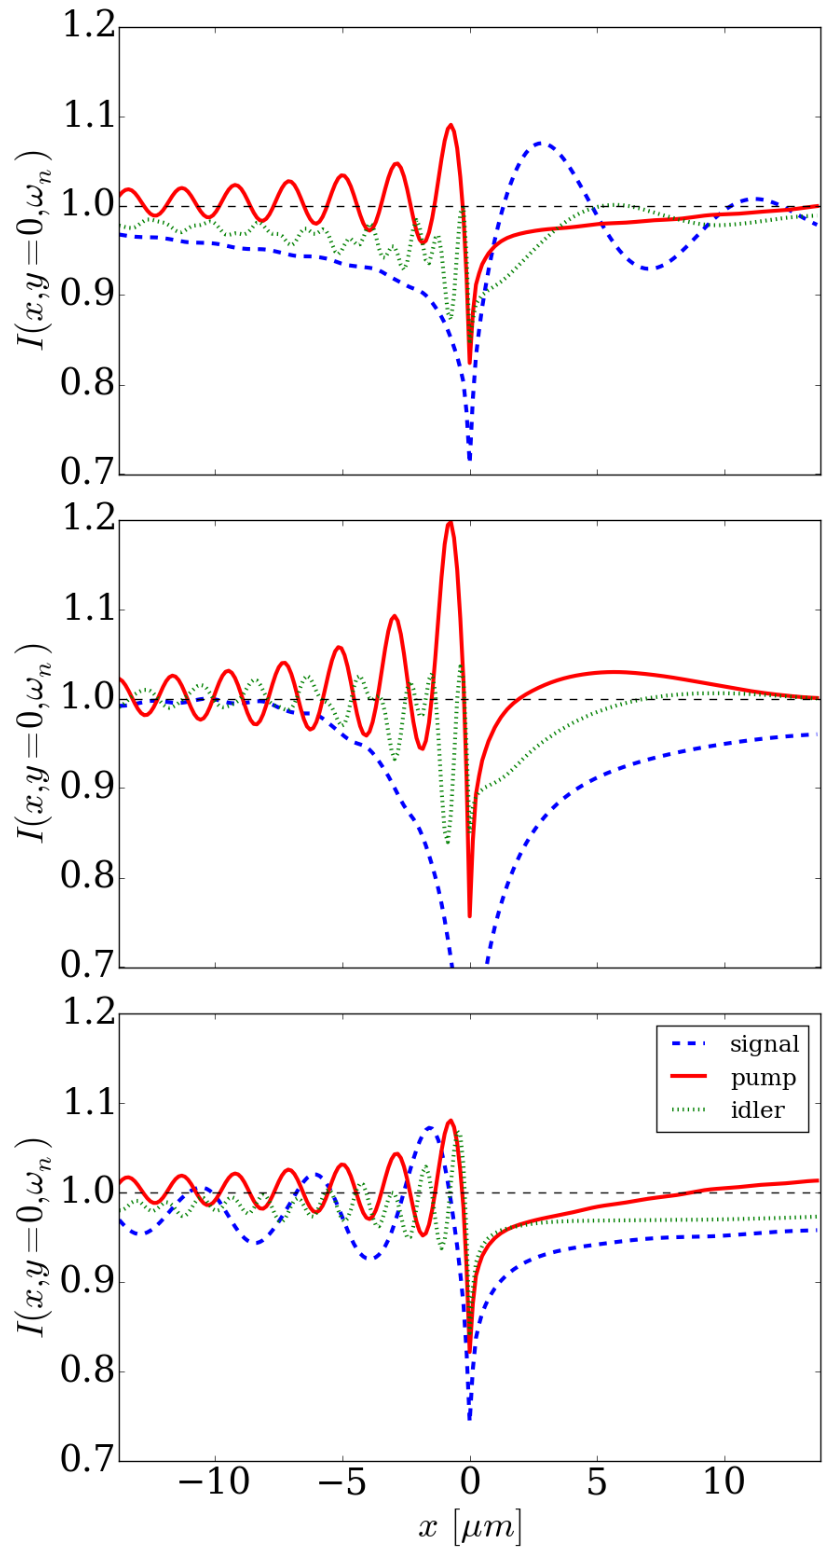
\includegraphics[width=.5\linewidth]{ranges.png}
% ~/notebooks/OPODrag/opodrag.py
\caption{Real space signal, pump and idler OPO one-dimensional
  filtered profiles in the linear-response approximation. OPO filtered
  emissions along the $y=0$ direction,
  $I (x, y=0, \omega_n) = |\psi(x,y=0, \omega_n)|^2/|\psi_n|^2$.  A
  signal at $k_s = -0.4$~$\mu$m$^{-1}$ (top panel) corresponds to
  Fig.~\ref{fig:ksm04}, a signal at $k_s = 0.0$~$\mu$m$^{-1}$ (middle
  panel) corresponds to Fig.~\ref{fig:ereal}, and a signal at
  $k_s = 0.7$~$\mu$m$^{-1}$ (bottom panel) corresponds to
  Fig.~\ref{fig:ksp07}. In each panel we plot the filtered profiles of
  signal, pump, and idler, while the horizontal gray dashed lines
  represent the values of the mean-field emission without a defect.}
\label{fig:range}
\end{figure}
%
\begin{figure}[tb]\centering
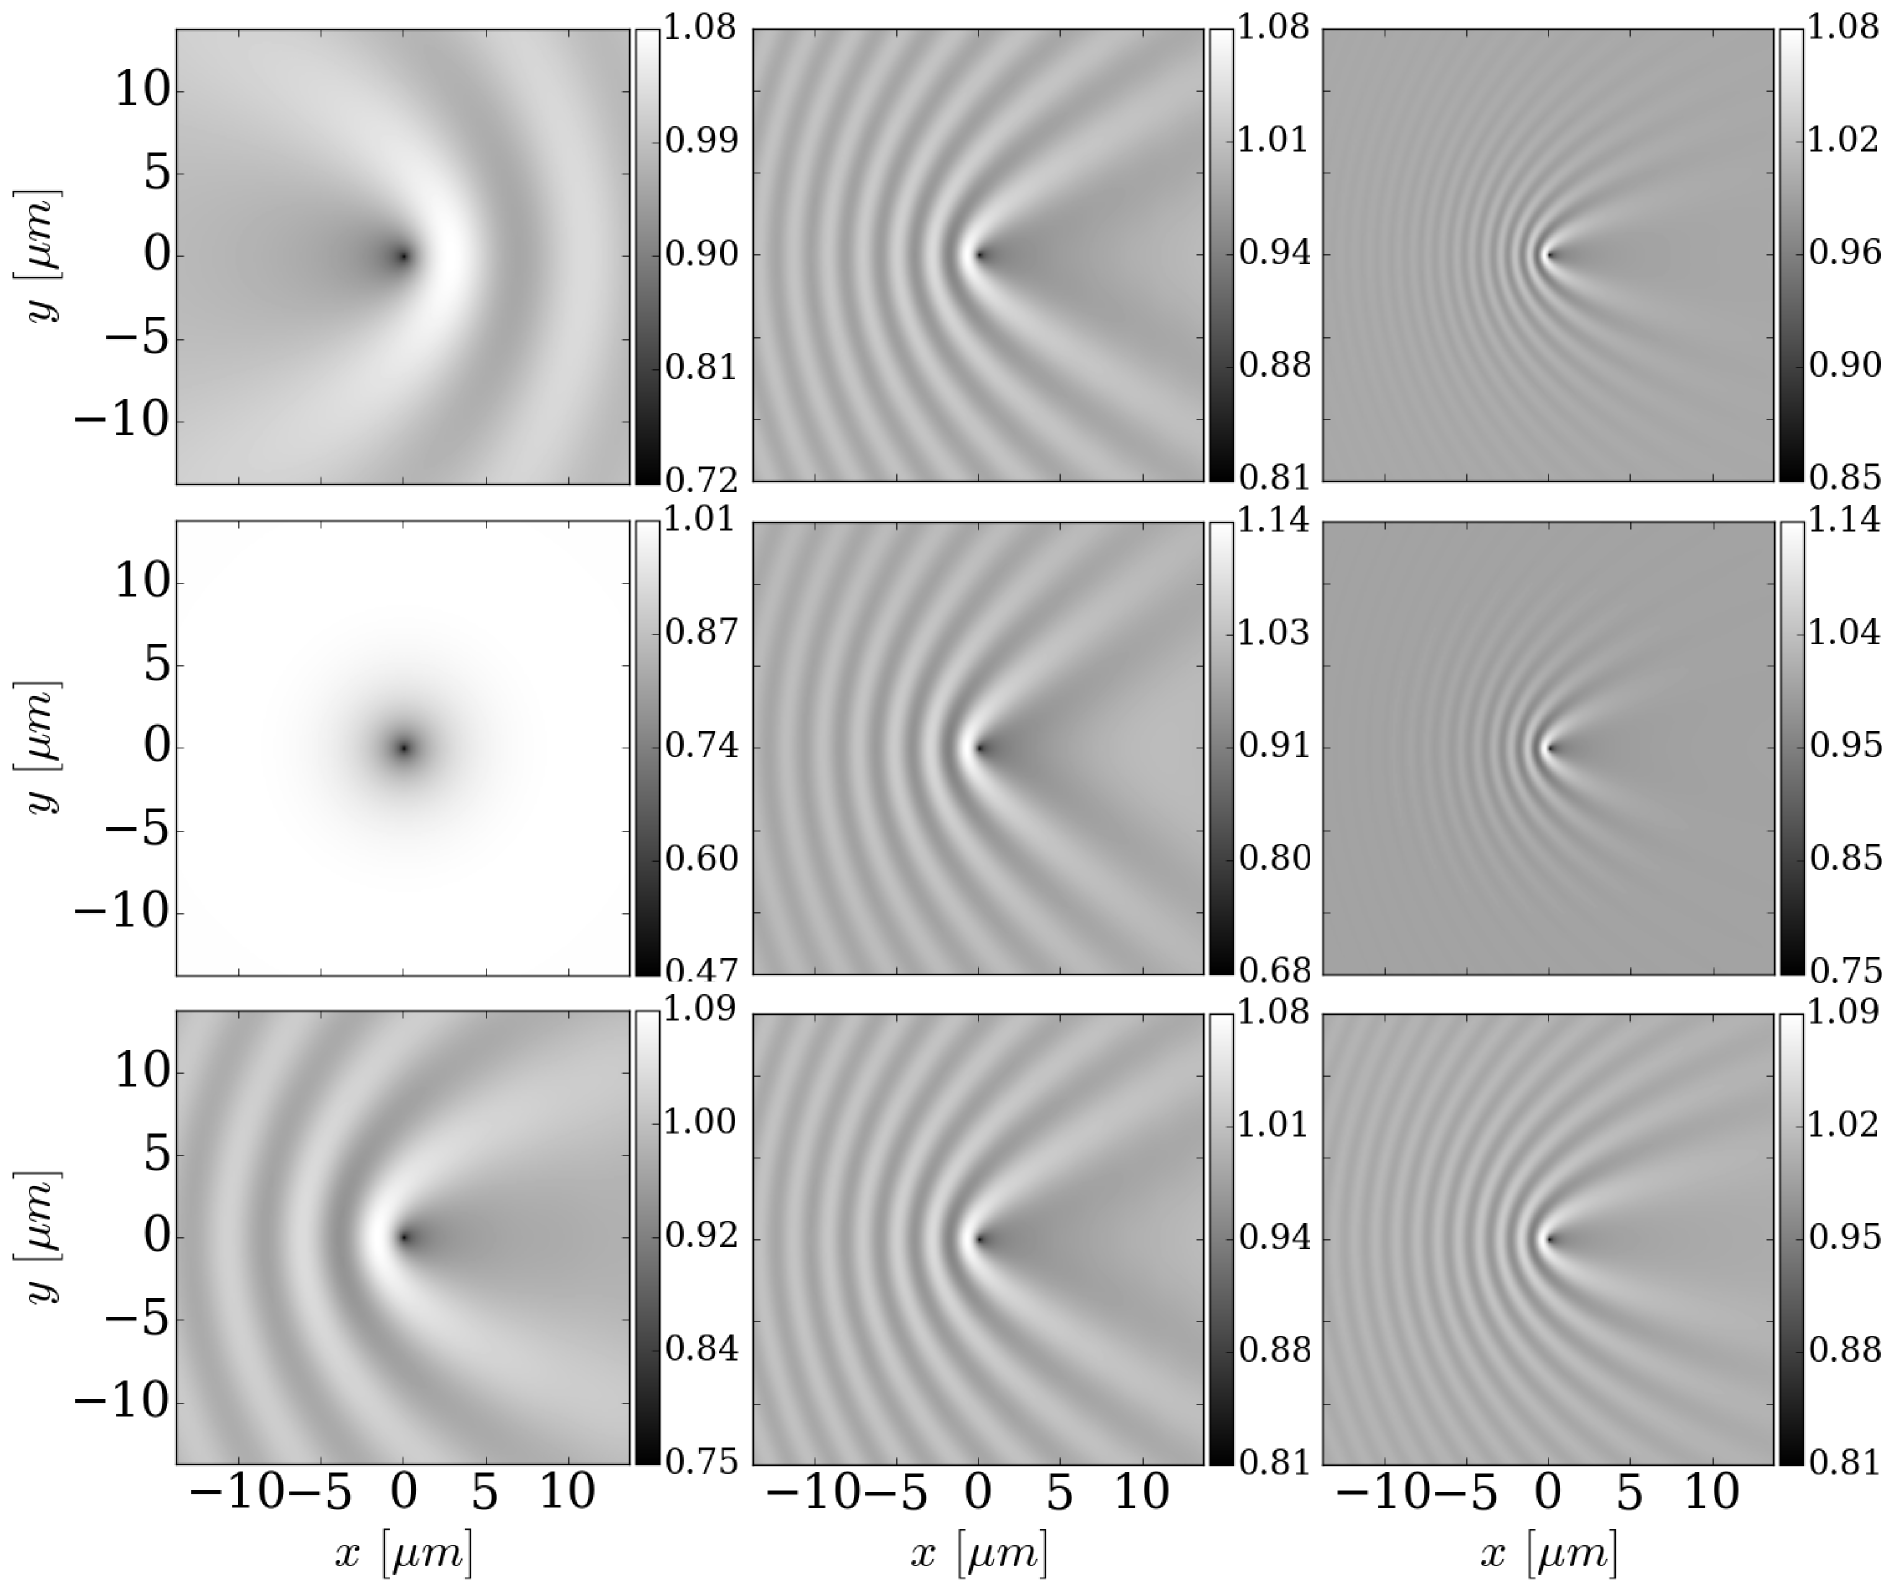
\includegraphics[width=.8\linewidth]{uncoupled.png}
% ~/notebooks/OPODrag/opodrag.py
\caption{Real space profiles of three uncoupled signal, pump and idler
  fluids. The rescaled profiles
  $|\psi (\vt{r},\omega_n)|^2/|\psi_n|^2$ are obtained by setting all
  off-diagonal couplings in Eq.~\eqref{eq:bogoliubov-opo} to zero,
  resulting in three uncoupled signal (left column), pump (middle
  column), and idler (right column) fluids. The three rows correspond
  to the three different cases previously analysed within the
  linear-response approximation: the case of a signal at
  $k_s = -0.4$~$\mu$m$^{-1}$ (top row) corresponds to the same
  conditions as Fig.~\ref{fig:ksm04}, a signal at
  $k_s = 0.0$~$\mu$m$^{-1}$ (middle row) corresponds to
  Fig.~\ref{fig:ereal}, and a signal at $k_s = 0.7$~$\mu$m$^{-1}$
  (bottom row) corresponds to Fig.~\ref{fig:ksp07}.}
\label{fig:uncou}
\end{figure}
%


\subsection{Linear response}
\label{subsec:analy}
%
In Chapter~\ref{cha:opo}, we also made use of the linear-response
approximation to analyse the OPO response to a static defect, valid
for a homogeneous pumping scheme. In order to do so, we first
evaluated the Bogoliubov matrix given in
Eq.~\eqref{eq:bogoliubov-opo}, whose eigenvalues determine the
spectrum of collective excitations. We plot in Fig.~\ref{fig:bogol} a
typical collective dispersion (here we consider the same system
parameters as the ones used in Fig.~\ref{fig:ereal}), by plotting the
real part of the Bogoliubov matrix eigenvalues
$\Re[\omega_{n,(u,v),\vt{k}-\vt{k}_n}]$ as a function of $k_x - k_n$
(cut at $k_y=0$). Note that the Rayleigh rings can be found by finding
the intersections $\Re[\omega_{n,(u,v),\vt{k}-\vt{k}_n}]=0$.

As also done for the full numerics, we consider a $\delta$-like
disorder potential $V_d(\vt{r}) = g_d \delta(\vt{r} - \vt{r}_0)$, and
Figs.~\ref{fig:spect} and~\ref{fig:ereal}, as well as
Figs.~\ref{fig:ksp07} and~\ref{fig:ksm04} below, are plotted for this
case.
%
We have checked that our results do not depend on the specific shape
of the defect potential: In particular, we have also considered the
response to defects with smooth Gaussian-like profiles, whose effect
is only to partially weaken the upstream modulations in real space.

We have seen in Chapter~\ref{cha:opo} that both experimentally as well
as in the full numerical analysis, one obtains OPO conditions where
the signal momentum is very close to zero, $\vt{k}_s \sim 0$. The
reason why OPO selects almost zero momentum signal conditions is still
awaiting a theoretical explaination.
%
In contrast, the linear-response approximation allows to access very
different OPO mean-field conditions, for which, by leaving unaltered
the value of the pump momentum, the signal can appear at finite
momentum values, either positive or negative.
%
This is a peculiarity of this approximation scheme, where one can show
that, at mean-field level, one has the possibility of choosing
different values of the signal momentum $\vt{k}_s$ (and thus the one
of the idler $\vt{k}_i$), and that this choice range is quite broad
particularly when the pump power is close to the lower pump threshold
for OPO --- the stability region for OPO is plotted as a shaded grey
region in the top left panels of Figs.~\ref{fig:ksp07}
and~\ref{fig:ksm04}. This is a well known ``selection problem'' for
parametric scattering (see Ref.~\cite{Wouters_2007_b}): The reason why
in full numerical calculations, parametric scattering processes select
a signal with a momentum close to zero, already very close to the
lower pump thresold for OPO, is still awaiting an explaination. In
particular, this quest cannot be addressed within a spatially
homogeneous approximation where the three mean-field solutions for
pump, signal, and idler states can be describes by plane waves.
%%
One can only show that, within the same mean-field approximation
scheme, when increasing the pump power towards the upper threshold for
OPO, the blue-shift of the LP polariton dispersion due to the
increasing mean-field polariton density, causes the signal momentum to
converge towards zero~\cite{Whittaker_2005} $\vt{k}_s \rightarrow 0$.

{\em{OPO with finite momentum signal--}} Given the freedom of choice for
the signal momentum $\vt{k}_s$ close to the lower OPO threshold, we
consider here two additional cases, that could not be studied neither
experimentally, nor within a full numerical approach, but that instead
we can easily analize within the linear-response theory.
%
In particular, we have left fixed the pumping conditions
$k_p=1.6$~$\mu$m$^{-1}$ and $\omega_p-\omega_X^0=-1.25$~meV and
considered two opposite situations.

In the first case, the signal has a finite and positive momentum $k_s
= 0.7$~$\mu$m$^{-1}$ and thus the idler is at low momentum, $k_i
=2.5$~$\mu$m$^{-1}$. The results are shown in Fig.~\ref{fig:ksp07}.
%
Here we see that all six Rayleigh rings are clearly visible and, in
addition, as the idler is at lower momentum compared to the case
considered in Figs.~\ref{fig:spect} and~\ref{fig:ereal}, and thus its
dispersion steeper, the idler group velocity is large enough to
appreciate the modulation of the Rayleigh ring associated to this
state. As a result, each of the three filtered OPO emissions exhibits
as the strongest modulation the one coming from its own Rayleigh ring,
including the signal which is now at finite and large momentum. In this
case, the OPO response of each filtered state profile looks completely
independent from the other, as if we were pumping each state
independently.

In the second case, shown in Fig.~\ref{fig:ksm04}, the signal is
finite and negative, $k_s = -0.4$~$\mu$m$^{-1}$, and the idler is now
at very large momentum, $k_i = 3.6$~$\mu$m$^{-1}$, where its
dispersion is very exciton-like and flat, and thus the idler has a
very small group velocity and its own modulations are visible only
very close to the defect. For this case, we can appreciate in the
idler filtered profile overlapped modulations from all the three state
Rayleigh rings (note that because the signal is at negative momentum,
its modulations have an opposite direction compared to the ones of
pump and idler), while in the signal we can mostly see the signal long
wavelength modulations and only very weakly the pump one.

We can compare the different modulation strengths of the three OPO
profiles by looking at the color bars plotted next to the profiles. In
order to better compare them on the same plot, we show in
Fig.~\ref{fig:range} the one-dimensional OPO filtered emissions along
the $y=0$ direction, rescaled by the mean-field solution $\psi_n$ in
absence of the defect, for the three cases analysed above. While for
the OPO conditions with a signal at $k_s = 0.0$~$\mu$m$^{-1}$ (middle
panel, corresponding to Fig.~\ref{fig:ereal}), the imprinted
modulations from the pump are hardly visible, and can only be
appreciated after a Gaussian filter manipulation, both OPO cases with
a finite momentum signal result in modulations in the signal with an
amplitude of the same order of magnitude of both pump and idler
fluids.

In Fig.~\ref{fig:uncou} we instead show the real space profiles
obtained by setting all off-diagonal couplings in the Bogoliubov
matrix $\mathcal{L}_{\vt{k}}$ of Eq.~\eqref{eq:bogoliubov-opo} to
zero, resulting in three uncoupled signal (left column), pump (middle
column), and idler (right column) fluids. This underlines the
importance of the coupling between the three fluids in the three
different OPO regimes previously analysed within the linear-response
approximation. In particular, for the OPO conditions such that the
signal has a finite and positive momentum $\vt{k}_s$ (bottom row of
Fig.~\ref{fig:uncou}, which corresponds to the conditions shown in
Fig.~\ref{fig:ksp07}), the coupling has little effect and the three
fluids respond to the defect in practice in a independent way (each
Rayleigh ring influences its own fluid). The OPO condition with a
finite and negative momentum $\vt{k}_s$, which corresponds to the
conditions shown in Fig.~\ref{fig:ksm04}, are shown in the top row of
Fig.~\ref{fig:uncou}: Here, we can see that the coupling between the
three fluids plays a role. The modulations of the pump can be
appreciated both in the signal profile (though weakly), as well as in
the idler profile. In the idler fluid its own modulations can only
propagate very close to the defect and thus the only really
appreciable modulations are the ones inherited from the pump. Finally,
for the experimentally relevant case of an OPO with a signal at zero
momentum (middle row of Fig.~\ref{fig:uncou}, which corresponds to the
conditions shown in Fig.~\ref{fig:ereal}), there is also a role played
by the coupling, though, as already thoroughly analysed, the
modulations in the signal inhereted from the pump can only be
appreciated after a Gaussian filtering manipulation.


Finally note that, as it also happens for the OPO conditions shown in
Fig.~\ref{fig:spect} of this Chapter, the subsonic to supersonic
crossover of the pump-only state~\cite{Amo_2009} happens at pump
intensities well above the region of stability of OPO --- the shaded
gray regions of Figs.~\ref{fig:ksp07} and~\ref{fig:ksm04} Thus, it is
not possible to study a case where the pump is already subsonic and at
the same time promotes stimulated scattering.

\section{Source code}\label{sec:source-code-opo}
%
This appendix contains \textsc{Python} 2.7 source code used for the
linear-response formalism in Chapter~\ref{cha:opo}, resulting in
Figs.~\ref{fig:spect}, \ref{fig:ereal}, \ref{fig:bogol},
\ref{fig:ksp07}, \ref{fig:ksm04}, \ref{fig:range},
and~\ref{fig:uncou}. The figures are plotted using the
\textsc{matplotlib} library v1.4.3, and the 3 coupled nonlinear
equations of state describing the OPO regime are solved using
\textsc{PHCpack} v2.3.86, a general-purpose solver for polynomial
systems, based on homotopy continuation methods.
%
%%%%%%%%%%%%%%%%%%%%%%%%%%%%%%%%%%%%%%%%%%%%%%%%%%%%%%%%%%%%%%%%%%%%%%%%%%%%
% export PYTHONPATH=/home/berceanu/tmp/yapf/                               %
% python2 tmp/yapf/yapf --in-place --style='{column_limit: 66}' opodrag.py %
% pygmentize -l python -f latex -o opodrag.tex opodrag.py                  %
%%%%%%%%%%%%%%%%%%%%%%%%%%%%%%%%%%%%%%%%%%%%%%%%%%%%%%%%%%%%%%%%%%%%%%%%%%%%

\begin{Verbatim}[commandchars=\\\{\}]
\PY{k+kn}{import} \PY{n+nn}{numpy} \PY{k+kn}{as} \PY{n+nn}{np}
\PY{k+kn}{import} \PY{n+nn}{matplotlib} \PY{k+kn}{as} \PY{n+nn}{mpl}
\PY{k+kn}{import} \PY{n+nn}{matplotlib.pyplot} \PY{k+kn}{as} \PY{n+nn}{plt}
\PY{k+kn}{import} \PY{n+nn}{matplotlib.cm} \PY{k+kn}{as} \PY{n+nn}{cm}
\PY{k+kn}{from} \PY{n+nn}{mpl\PYZus{}toolkits.mplot3d} \PY{k+kn}{import} \PY{n}{Axes3D}
\PY{c+c1}{\PYZsh{} for colorbar stuff}
\PY{k+kn}{from} \PY{n+nn}{mpl\PYZus{}toolkits.axes\PYZus{}grid1} \PY{k+kn}{import} \PY{n}{make\PYZus{}axes\PYZus{}locatable}
\PY{k+kn}{from} \PY{n+nn}{matplotlib} \PY{k+kn}{import} \PY{n}{ticker}
\PY{k+kn}{from} \PY{n+nn}{scipy} \PY{k+kn}{import} \PY{n}{optimize}
\PY{k+kn}{from} \PY{n+nn}{phcpy.phcpy2c} \PY{k+kn}{import} \PY{n}{py2c\PYZus{}set\PYZus{}seed}
\PY{k+kn}{from} \PY{n+nn}{phcpy.solver} \PY{k+kn}{import} \PY{n}{solve}
\PY{k+kn}{from} \PY{n+nn}{phcpy.solutions} \PY{k+kn}{import} \PY{n}{strsol2dict}
\PY{k+kn}{import} \PY{n+nn}{ConfigParser}
\PY{k+kn}{import} \PY{n+nn}{sys}
\PY{k}{def} \PY{n+nf}{read\PYZus{}parameters}\PY{p}{(}\PY{n}{filename}\PY{p}{)}\PY{p}{:}
    \PY{n}{config} \PY{o}{=} \PY{n}{ConfigParser}\PY{o}{.}\PY{n}{RawConfigParser}\PY{p}{(}\PY{p}{)}
    \PY{k}{try}\PY{p}{:}
        \PY{n}{config}\PY{o}{.}\PY{n}{readfp}\PY{p}{(}\PY{n+nb}{open}\PY{p}{(}\PY{n}{filename}\PY{p}{)}\PY{p}{)}
    \PY{k}{except} \PY{n+ne}{IOError}\PY{p}{:}
        \PY{k}{raise} \PY{n+ne}{IOError}\PY{p}{(}\PY{l+s+s1}{\PYZsq{}}\PY{l+s+s1}{cannot find parameters.ini, exiting}\PY{l+s+s1}{\PYZsq{}}\PY{p}{)}
    \PY{k}{return} \PY{n}{config}
\PY{n}{param} \PY{o}{=} \PY{n}{read\PYZus{}parameters}\PY{p}{(}
    \PY{l+s+s2}{\PYZdq{}}\PY{l+s+s2}{/home/berceanu/notebooks/OPODrag/parameters.ini}\PY{l+s+s2}{\PYZdq{}}\PY{p}{)}
\PY{n}{param\PYZus{}set} \PY{o}{=} \PY{n}{sys}\PY{o}{.}\PY{n}{argv}\PY{p}{[}\PY{l+m+mi}{1}\PY{p}{]}
\PY{n}{omega\PYZus{}X} \PY{o}{=} \PY{n}{param}\PY{o}{.}\PY{n}{getfloat}\PY{p}{(}\PY{n}{param\PYZus{}set}\PY{p}{,} \PY{l+s+s2}{\PYZdq{}}\PY{l+s+s2}{omega\PYZus{}X}\PY{l+s+s2}{\PYZdq{}}\PY{p}{)}
\PY{n}{omega\PYZus{}C0} \PY{o}{=} \PY{n}{param}\PY{o}{.}\PY{n}{getfloat}\PY{p}{(}\PY{n}{param\PYZus{}set}\PY{p}{,} \PY{l+s+s2}{\PYZdq{}}\PY{l+s+s2}{omega\PYZus{}C0}\PY{l+s+s2}{\PYZdq{}}\PY{p}{)}
\PY{n}{kz} \PY{o}{=} \PY{n}{param}\PY{o}{.}\PY{n}{getfloat}\PY{p}{(}\PY{n}{param\PYZus{}set}\PY{p}{,} \PY{l+s+s2}{\PYZdq{}}\PY{l+s+s2}{kz}\PY{l+s+s2}{\PYZdq{}}\PY{p}{)}
\PY{n}{Omega\PYZus{}R} \PY{o}{=} \PY{n}{param}\PY{o}{.}\PY{n}{getfloat}\PY{p}{(}\PY{n}{param\PYZus{}set}\PY{p}{,} \PY{l+s+s2}{\PYZdq{}}\PY{l+s+s2}{Omega\PYZus{}R}\PY{l+s+s2}{\PYZdq{}}\PY{p}{)}
\PY{n}{gamma\PYZus{}X} \PY{o}{=} \PY{n}{param}\PY{o}{.}\PY{n}{getfloat}\PY{p}{(}\PY{n}{param\PYZus{}set}\PY{p}{,} \PY{l+s+s2}{\PYZdq{}}\PY{l+s+s2}{gamma\PYZus{}X}\PY{l+s+s2}{\PYZdq{}}\PY{p}{)}
\PY{n}{gamma\PYZus{}C} \PY{o}{=} \PY{n}{param}\PY{o}{.}\PY{n}{getfloat}\PY{p}{(}\PY{n}{param\PYZus{}set}\PY{p}{,} \PY{l+s+s2}{\PYZdq{}}\PY{l+s+s2}{gamma\PYZus{}C}\PY{l+s+s2}{\PYZdq{}}\PY{p}{)}
\PY{n}{k\PYZus{}pmpx} \PY{o}{=} \PY{n}{param}\PY{o}{.}\PY{n}{getfloat}\PY{p}{(}\PY{n}{param\PYZus{}set}\PY{p}{,} \PY{l+s+s2}{\PYZdq{}}\PY{l+s+s2}{k\PYZus{}pmpx}\PY{l+s+s2}{\PYZdq{}}\PY{p}{)}
\PY{n}{k\PYZus{}pmpy} \PY{o}{=} \PY{n}{param}\PY{o}{.}\PY{n}{getfloat}\PY{p}{(}\PY{n}{param\PYZus{}set}\PY{p}{,} \PY{l+s+s2}{\PYZdq{}}\PY{l+s+s2}{k\PYZus{}pmpy}\PY{l+s+s2}{\PYZdq{}}\PY{p}{)}
\PY{n}{k\PYZus{}sigx} \PY{o}{=} \PY{n}{param}\PY{o}{.}\PY{n}{getfloat}\PY{p}{(}\PY{n}{param\PYZus{}set}\PY{p}{,} \PY{l+s+s2}{\PYZdq{}}\PY{l+s+s2}{k\PYZus{}sigx}\PY{l+s+s2}{\PYZdq{}}\PY{p}{)}
\PY{n}{k\PYZus{}sigy} \PY{o}{=} \PY{n}{param}\PY{o}{.}\PY{n}{getfloat}\PY{p}{(}\PY{n}{param\PYZus{}set}\PY{p}{,} \PY{l+s+s2}{\PYZdq{}}\PY{l+s+s2}{k\PYZus{}sigy}\PY{l+s+s2}{\PYZdq{}}\PY{p}{)}
\PY{n}{omega\PYZus{}pmp} \PY{o}{=} \PY{n}{param}\PY{o}{.}\PY{n}{getfloat}\PY{p}{(}\PY{n}{param\PYZus{}set}\PY{p}{,} \PY{l+s+s2}{\PYZdq{}}\PY{l+s+s2}{omega\PYZus{}pmp}\PY{l+s+s2}{\PYZdq{}}\PY{p}{)}
\PY{n}{ip\PYZus{}chosen} \PY{o}{=} \PY{n}{param}\PY{o}{.}\PY{n}{getfloat}\PY{p}{(}\PY{n}{param\PYZus{}set}\PY{p}{,} \PY{l+s+s2}{\PYZdq{}}\PY{l+s+s2}{ip\PYZus{}chosen}\PY{l+s+s2}{\PYZdq{}}\PY{p}{)}
\PY{n}{gv} \PY{o}{=} \PY{n}{param}\PY{o}{.}\PY{n}{getfloat}\PY{p}{(}\PY{n}{param\PYZus{}set}\PY{p}{,} \PY{l+s+s2}{\PYZdq{}}\PY{l+s+s2}{gv}\PY{l+s+s2}{\PYZdq{}}\PY{p}{)}
\PY{n}{nkx} \PY{o}{=} \PY{n}{param}\PY{o}{.}\PY{n}{getfloat}\PY{p}{(}\PY{n}{param\PYZus{}set}\PY{p}{,} \PY{l+s+s2}{\PYZdq{}}\PY{l+s+s2}{nkx}\PY{l+s+s2}{\PYZdq{}}\PY{p}{)}
\PY{n}{nky} \PY{o}{=} \PY{n}{param}\PY{o}{.}\PY{n}{getfloat}\PY{p}{(}\PY{n}{param\PYZus{}set}\PY{p}{,} \PY{l+s+s2}{\PYZdq{}}\PY{l+s+s2}{nky}\PY{l+s+s2}{\PYZdq{}}\PY{p}{)}
\PY{n}{ipx\PYZus{}start} \PY{o}{=} \PY{n}{param}\PY{o}{.}\PY{n}{getfloat}\PY{p}{(}\PY{n}{param\PYZus{}set}\PY{p}{,} \PY{l+s+s2}{\PYZdq{}}\PY{l+s+s2}{ipx\PYZus{}start}\PY{l+s+s2}{\PYZdq{}}\PY{p}{)}
\PY{n}{ipx\PYZus{}end} \PY{o}{=} \PY{n}{param}\PY{o}{.}\PY{n}{getfloat}\PY{p}{(}\PY{n}{param\PYZus{}set}\PY{p}{,} \PY{l+s+s2}{\PYZdq{}}\PY{l+s+s2}{ipx\PYZus{}end}\PY{l+s+s2}{\PYZdq{}}\PY{p}{)}
\PY{n}{kxl} \PY{o}{=} \PY{n}{param}\PY{o}{.}\PY{n}{getfloat}\PY{p}{(}\PY{n}{param\PYZus{}set}\PY{p}{,} \PY{l+s+s2}{\PYZdq{}}\PY{l+s+s2}{kxl}\PY{l+s+s2}{\PYZdq{}}\PY{p}{)}
\PY{n}{kxr} \PY{o}{=} \PY{n}{param}\PY{o}{.}\PY{n}{getfloat}\PY{p}{(}\PY{n}{param\PYZus{}set}\PY{p}{,} \PY{l+s+s2}{\PYZdq{}}\PY{l+s+s2}{kxr}\PY{l+s+s2}{\PYZdq{}}\PY{p}{)}
\PY{n}{kyl} \PY{o}{=} \PY{n}{param}\PY{o}{.}\PY{n}{getfloat}\PY{p}{(}\PY{n}{param\PYZus{}set}\PY{p}{,} \PY{l+s+s2}{\PYZdq{}}\PY{l+s+s2}{kyl}\PY{l+s+s2}{\PYZdq{}}\PY{p}{)}
\PY{n}{kyr} \PY{o}{=} \PY{n}{param}\PY{o}{.}\PY{n}{getfloat}\PY{p}{(}\PY{n}{param\PYZus{}set}\PY{p}{,} \PY{l+s+s2}{\PYZdq{}}\PY{l+s+s2}{kyr}\PY{l+s+s2}{\PYZdq{}}\PY{p}{)}
\PY{n}{eigs\PYZus{}threshold} \PY{o}{=} \PY{n}{param}\PY{o}{.}\PY{n}{getfloat}\PY{p}{(}\PY{n}{param\PYZus{}set}\PY{p}{,} \PY{l+s+s2}{\PYZdq{}}\PY{l+s+s2}{eigs\PYZus{}threshold}\PY{l+s+s2}{\PYZdq{}}\PY{p}{)}
\PY{n}{stride\PYZus{}r} \PY{o}{=} \PY{n}{param}\PY{o}{.}\PY{n}{getint}\PY{p}{(}\PY{n}{param\PYZus{}set}\PY{p}{,} \PY{l+s+s2}{\PYZdq{}}\PY{l+s+s2}{stride\PYZus{}r}\PY{l+s+s2}{\PYZdq{}}\PY{p}{)}
\PY{n}{stride\PYZus{}c} \PY{o}{=} \PY{n}{param}\PY{o}{.}\PY{n}{getint}\PY{p}{(}\PY{n}{param\PYZus{}set}\PY{p}{,} \PY{l+s+s2}{\PYZdq{}}\PY{l+s+s2}{stride\PYZus{}c}\PY{l+s+s2}{\PYZdq{}}\PY{p}{)}
\PY{n}{delta\PYZus{}k} \PY{o}{=} \PY{n}{param}\PY{o}{.}\PY{n}{getfloat}\PY{p}{(}\PY{n}{param\PYZus{}set}\PY{p}{,} \PY{l+s+s2}{\PYZdq{}}\PY{l+s+s2}{delta\PYZus{}k}\PY{l+s+s2}{\PYZdq{}}\PY{p}{)}
\PY{n}{ipstabini} \PY{o}{=} \PY{n}{param}\PY{o}{.}\PY{n}{getfloat}\PY{p}{(}\PY{n}{param\PYZus{}set}\PY{p}{,} \PY{l+s+s2}{\PYZdq{}}\PY{l+s+s2}{ipstabini}\PY{l+s+s2}{\PYZdq{}}\PY{p}{)}
\PY{n}{ipstabfin} \PY{o}{=} \PY{n}{param}\PY{o}{.}\PY{n}{getfloat}\PY{p}{(}\PY{n}{param\PYZus{}set}\PY{p}{,} \PY{l+s+s2}{\PYZdq{}}\PY{l+s+s2}{ipstabfin}\PY{l+s+s2}{\PYZdq{}}\PY{p}{)}
\PY{n}{k\PYZus{}idlx} \PY{o}{=} \PY{l+m+mi}{2} \PY{o}{*} \PY{n}{k\PYZus{}pmpx} \PY{o}{\PYZhy{}} \PY{n}{k\PYZus{}sigx}
\PY{n}{k\PYZus{}idly} \PY{o}{=} \PY{l+m+mi}{2} \PY{o}{*} \PY{n}{k\PYZus{}pmpy} \PY{o}{\PYZhy{}} \PY{n}{k\PYZus{}sigy}
\PY{n}{ks} \PY{o}{=} \PY{p}{(}\PY{l+s+s2}{\PYZdq{}}\PY{l+s+s2}{\PYZob{}0:.3f\PYZcb{}}\PY{l+s+s2}{\PYZdq{}}\PY{o}{.}\PY{n}{format}\PY{p}{(}\PY{n}{k\PYZus{}sigx}\PY{p}{)}\PY{p}{)}\PY{o}{.}\PY{n}{replace}\PY{p}{(}\PY{l+s+s2}{\PYZdq{}}\PY{l+s+s2}{.}\PY{l+s+s2}{\PYZdq{}}\PY{p}{,} \PY{l+s+s2}{\PYZdq{}}\PY{l+s+s2}{\PYZus{}}\PY{l+s+s2}{\PYZdq{}}\PY{p}{)}
\PY{n}{gp} \PY{o}{=} \PY{n}{gamma\PYZus{}C} \PY{o}{+} \PY{p}{(}\PY{l+m+mi}{1} \PY{o}{/} \PY{n}{np}\PY{o}{.}\PY{n}{sqrt}\PY{p}{(}\PY{l+m+mi}{1} \PY{o}{+} \PY{p}{(}\PY{n}{Omega\PYZus{}R} \PY{o}{/} \PY{p}{(}
    \PY{p}{(}\PY{l+m+mf}{0.5} \PY{o}{*} \PY{p}{(}\PY{p}{(}\PY{n}{omega\PYZus{}C0} \PY{o}{*} \PY{n}{np}\PY{o}{.}\PY{n}{sqrt}\PY{p}{(}\PY{l+m+mi}{1} \PY{o}{+} \PY{p}{(}\PY{n}{np}\PY{o}{.}\PY{n}{sqrt}\PY{p}{(}
        \PY{n}{k\PYZus{}pmpx}\PY{o}{*}\PY{o}{*}\PY{l+m+mi}{2} \PY{o}{+} \PY{n}{k\PYZus{}pmpy}\PY{o}{*}\PY{o}{*}\PY{l+m+mi}{2}\PY{p}{)} \PY{o}{/} \PY{n}{kz}\PY{p}{)}\PY{o}{*}\PY{o}{*}\PY{l+m+mi}{2}\PY{p}{)}\PY{p}{)} \PY{o}{+} \PY{n}{omega\PYZus{}X}\PY{p}{)} \PY{o}{\PYZhy{}} \PY{l+m+mf}{0.5} \PY{o}{*}
     \PY{n}{np}\PY{o}{.}\PY{n}{sqrt}\PY{p}{(}\PY{p}{(}\PY{p}{(}\PY{n}{omega\PYZus{}C0} \PY{o}{*} \PY{n}{np}\PY{o}{.}\PY{n}{sqrt}\PY{p}{(}\PY{l+m+mi}{1} \PY{o}{+} \PY{p}{(}\PY{n}{np}\PY{o}{.}\PY{n}{sqrt}\PY{p}{(}
         \PY{n}{k\PYZus{}pmpx}\PY{o}{*}\PY{o}{*}\PY{l+m+mi}{2} \PY{o}{+} \PY{n}{k\PYZus{}pmpy}\PY{o}{*}\PY{o}{*}\PY{l+m+mi}{2}\PY{p}{)} \PY{o}{/} \PY{n}{kz}\PY{p}{)}\PY{o}{*}\PY{o}{*}\PY{l+m+mi}{2}\PY{p}{)}\PY{p}{)} \PY{o}{\PYZhy{}} \PY{n}{omega\PYZus{}X}\PY{p}{)}\PY{o}{*}\PY{o}{*}\PY{l+m+mi}{2} \PY{o}{+} \PY{l+m+mi}{4} \PY{o}{*}
             \PY{n}{Omega\PYZus{}R}\PY{o}{*}\PY{o}{*}\PY{l+m+mi}{2}\PY{p}{)}\PY{p}{)} \PY{o}{\PYZhy{}} \PY{p}{(}\PY{n}{omega\PYZus{}C0} \PY{o}{*} \PY{n}{np}\PY{o}{.}\PY{n}{sqrt}\PY{p}{(}\PY{l+m+mi}{1} \PY{o}{+} \PY{p}{(}\PY{n}{np}\PY{o}{.}\PY{n}{sqrt}\PY{p}{(}
                 \PY{n}{k\PYZus{}pmpx}\PY{o}{*}\PY{o}{*}\PY{l+m+mi}{2} \PY{o}{+} \PY{n}{k\PYZus{}pmpy}\PY{o}{*}\PY{o}{*}\PY{l+m+mi}{2}\PY{p}{)} \PY{o}{/} \PY{n}{kz}\PY{p}{)}\PY{o}{*}\PY{o}{*}\PY{l+m+mi}{2}\PY{p}{)}\PY{p}{)}\PY{p}{)}\PY{p}{)}\PY{o}{*}\PY{o}{*}\PY{l+m+mi}{2}\PY{p}{)}\PY{p}{)}\PY{o}{*}\PY{o}{*}\PY{l+m+mi}{2} \PY{o}{*} \PY{p}{(}
                     \PY{n}{gamma\PYZus{}X} \PY{o}{\PYZhy{}} \PY{n}{gamma\PYZus{}C}\PY{p}{)}
\PY{n}{omega\PYZus{}p\PYZus{}chosen} \PY{o}{=} \PY{p}{(}\PY{n}{omega\PYZus{}pmp} \PY{o}{\PYZhy{}} \PY{n}{omega\PYZus{}X}\PY{p}{)} \PY{o}{/} \PY{n}{gp}
\PY{n}{side\PYZus{}k} \PY{o}{=} \PY{n}{nkx} \PY{o}{*} \PY{n}{delta\PYZus{}k} \PY{o}{/} \PY{l+m+mi}{2}
\PY{n}{side\PYZus{}r} \PY{o}{=} \PY{n}{np}\PY{o}{.}\PY{n}{pi} \PY{o}{/} \PY{n}{delta\PYZus{}k}
\PY{n}{delta\PYZus{}r} \PY{o}{=} \PY{n}{np}\PY{o}{.}\PY{n}{pi} \PY{o}{/} \PY{n}{side\PYZus{}k}
\PY{n}{x} \PY{o}{=} \PY{n}{y} \PY{o}{=} \PY{n}{np}\PY{o}{.}\PY{n}{arange}\PY{p}{(}\PY{o}{\PYZhy{}}\PY{n}{side\PYZus{}r}\PY{p}{,} \PY{n}{side\PYZus{}r}\PY{p}{,} \PY{n}{delta\PYZus{}r}\PY{p}{)}
\PY{n}{kx} \PY{o}{=} \PY{n}{ky} \PY{o}{=} \PY{n}{np}\PY{o}{.}\PY{n}{arange}\PY{p}{(}\PY{o}{\PYZhy{}}\PY{n}{side\PYZus{}k}\PY{p}{,} \PY{n}{side\PYZus{}k}\PY{p}{,} \PY{n}{delta\PYZus{}k}\PY{p}{)}
\PY{n}{KX}\PY{p}{,} \PY{n}{KY} \PY{o}{=} \PY{n}{np}\PY{o}{.}\PY{n}{meshgrid}\PY{p}{(}\PY{n}{kx}\PY{p}{,} \PY{n}{ky}\PY{p}{)}
\PY{n}{X}\PY{p}{,} \PY{n}{Y} \PY{o}{=} \PY{n}{np}\PY{o}{.}\PY{n}{meshgrid}\PY{p}{(}\PY{n}{x}\PY{p}{,} \PY{n}{y}\PY{p}{)}
\PY{n}{ipx} \PY{o}{=} \PY{n}{np}\PY{o}{.}\PY{n}{linspace}\PY{p}{(}\PY{n}{ipx\PYZus{}start}\PY{p}{,} \PY{n}{ipx\PYZus{}end}\PY{p}{,} \PY{l+m+mi}{30}\PY{p}{)}
\PY{n}{mpl}\PY{o}{.}\PY{n}{rcParams}\PY{o}{.}\PY{n}{update}\PY{p}{(}\PY{p}{\PYZob{}}\PY{l+s+s1}{\PYZsq{}}\PY{l+s+s1}{font.size}\PY{l+s+s1}{\PYZsq{}}\PY{p}{:} \PY{l+m+mi}{28}\PY{p}{,} \PY{l+s+s1}{\PYZsq{}}\PY{l+s+s1}{font.family}\PY{l+s+s1}{\PYZsq{}}\PY{p}{:} \PY{l+s+s1}{\PYZsq{}}\PY{l+s+s1}{serif}\PY{l+s+s1}{\PYZsq{}}\PY{p}{\PYZcb{}}\PY{p}{)}
\PY{n}{x\PYZus{}label\PYZus{}k} \PY{o}{=} \PY{l+s+s1}{r\PYZsq{}}\PY{l+s+s1}{\PYZdl{}k\PYZus{}x \PYZhy{} k\PYZus{}n}\PY{l+s+s1}{\PYZbs{}}\PY{l+s+s1}{,[}\PY{l+s+s1}{\PYZbs{}}\PY{l+s+s1}{mu m\PYZca{}\PYZob{}\PYZhy{}1\PYZcb{}]\PYZdl{}}\PY{l+s+s1}{\PYZsq{}}
\PY{n}{y\PYZus{}label\PYZus{}k} \PY{o}{=} \PY{l+s+s1}{r\PYZsq{}}\PY{l+s+s1}{\PYZdl{}k\PYZus{}y}\PY{l+s+s1}{\PYZbs{}}\PY{l+s+s1}{,[}\PY{l+s+s1}{\PYZbs{}}\PY{l+s+s1}{mu m\PYZca{}\PYZob{}\PYZhy{}1\PYZcb{}]\PYZdl{}}\PY{l+s+s1}{\PYZsq{}}
\PY{n}{x\PYZus{}label\PYZus{}i} \PY{o}{=} \PY{l+s+s1}{r\PYZsq{}}\PY{l+s+s1}{\PYZdl{}x}\PY{l+s+s1}{\PYZbs{}}\PY{l+s+s1}{,[}\PY{l+s+s1}{\PYZbs{}}\PY{l+s+s1}{mu m]\PYZdl{}}\PY{l+s+s1}{\PYZsq{}}
\PY{n}{y\PYZus{}label\PYZus{}i} \PY{o}{=} \PY{l+s+s1}{r\PYZsq{}}\PY{l+s+s1}{\PYZdl{}y}\PY{l+s+s1}{\PYZbs{}}\PY{l+s+s1}{,[}\PY{l+s+s1}{\PYZbs{}}\PY{l+s+s1}{mu m]\PYZdl{}}\PY{l+s+s1}{\PYZsq{}}
\PY{n}{letter\PYZus{}spi} \PY{o}{=} \PY{p}{[}\PY{l+s+s1}{\PYZsq{}}\PY{l+s+s1}{s}\PY{l+s+s1}{\PYZsq{}}\PY{p}{,} \PY{l+s+s1}{\PYZsq{}}\PY{l+s+s1}{p}\PY{l+s+s1}{\PYZsq{}}\PY{p}{,} \PY{l+s+s1}{\PYZsq{}}\PY{l+s+s1}{i}\PY{l+s+s1}{\PYZsq{}}\PY{p}{]}
\PY{n}{title\PYZus{}k} \PY{o}{=} \PY{p}{[}\PY{p}{]}
\PY{k}{for} \PY{n}{idx} \PY{o+ow}{in} \PY{n+nb}{range}\PY{p}{(}\PY{l+m+mi}{3}\PY{p}{)}\PY{p}{:}
    \PY{n}{title\PYZus{}k}\PY{o}{.}\PY{n}{append}\PY{p}{(}\PY{l+s+s1}{r\PYZsq{}}\PY{l+s+s1}{\PYZdl{}g }\PY{l+s+s1}{\PYZbs{}}\PY{l+s+s1}{left|}\PY{l+s+s1}{\PYZbs{}}\PY{l+s+s1}{tilde\PYZob{}}\PY{l+s+s1}{\PYZbs{}}\PY{l+s+s1}{Psi\PYZcb{}\PYZus{}\PYZob{}LP\PYZcb{}\PYZca{}\PYZob{}}\PY{l+s+s1}{\PYZsq{}} \PY{o}{+} \PY{n}{letter\PYZus{}spi}\PY{p}{[}
        \PY{n}{idx}\PY{p}{]} \PY{o}{+} \PY{l+s+s1}{r\PYZsq{}}\PY{l+s+s1}{\PYZcb{}}\PY{l+s+s1}{\PYZbs{}}\PY{l+s+s1}{left(k+k\PYZus{}\PYZob{}}\PY{l+s+s1}{\PYZsq{}} \PY{o}{+} \PY{n}{letter\PYZus{}spi}\PY{p}{[}\PY{n}{idx}\PY{p}{]} \PY{o}{+}
                   \PY{l+s+s1}{r\PYZsq{}}\PY{l+s+s1}{\PYZcb{}}\PY{l+s+s1}{\PYZbs{}}\PY{l+s+s1}{right)}\PY{l+s+s1}{\PYZbs{}}\PY{l+s+s1}{right|\PYZca{}\PYZob{}2\PYZcb{} [}\PY{l+s+s1}{\PYZbs{}}\PY{l+s+s1}{gamma\PYZus{}p }\PY{l+s+s1}{\PYZbs{}}\PY{l+s+s1}{mu m\PYZca{}4]\PYZdl{}}\PY{l+s+s1}{\PYZsq{}}\PY{p}{)}
\PY{n}{title\PYZus{}i} \PY{o}{=} \PY{p}{[}\PY{p}{]}
\PY{k}{for} \PY{n}{idx} \PY{o+ow}{in} \PY{n+nb}{range}\PY{p}{(}\PY{l+m+mi}{3}\PY{p}{)}\PY{p}{:}
    \PY{n}{title\PYZus{}i}\PY{o}{.}\PY{n}{append}\PY{p}{(}\PY{l+s+s1}{r\PYZsq{}}\PY{l+s+s1}{\PYZdl{}I\PYZca{}}\PY{l+s+s1}{\PYZsq{}} \PY{o}{+} \PY{n}{letter\PYZus{}spi}\PY{p}{[}\PY{n}{idx}\PY{p}{]} \PY{o}{+} \PY{l+s+s1}{r\PYZsq{}}\PY{l+s+s1}{\PYZdl{}}\PY{l+s+s1}{\PYZsq{}}\PY{p}{)}
\PY{n}{color\PYZus{}spi} \PY{o}{=} \PY{p}{[}\PY{l+s+s1}{\PYZsq{}}\PY{l+s+s1}{blue}\PY{l+s+s1}{\PYZsq{}}\PY{p}{,} \PY{l+s+s1}{\PYZsq{}}\PY{l+s+s1}{red}\PY{l+s+s1}{\PYZsq{}}\PY{p}{,} \PY{l+s+s1}{\PYZsq{}}\PY{l+s+s1}{green}\PY{l+s+s1}{\PYZsq{}}\PY{p}{]}
\PY{n}{marker\PYZus{}spi} \PY{o}{=} \PY{p}{[}\PY{l+s+s1}{\PYZsq{}}\PY{l+s+s1}{\PYZca{}}\PY{l+s+s1}{\PYZsq{}}\PY{p}{,} \PY{l+s+s1}{\PYZsq{}}\PY{l+s+s1}{o}\PY{l+s+s1}{\PYZsq{}}\PY{p}{,} \PY{l+s+s1}{\PYZsq{}}\PY{l+s+s1}{v}\PY{l+s+s1}{\PYZsq{}}\PY{p}{]}
\PY{n}{momentum\PYZus{}spi} \PY{o}{=} \PY{n}{np}\PY{o}{.}\PY{n}{array}\PY{p}{(}\PY{p}{[}\PY{p}{[}\PY{n}{k\PYZus{}sigx}\PY{p}{,} \PY{n}{k\PYZus{}sigy}\PY{p}{]}\PY{p}{,} \PY{p}{[}\PY{n}{k\PYZus{}pmpx}\PY{p}{,} \PY{n}{k\PYZus{}pmpy}\PY{p}{]}\PY{p}{,}
                         \PY{p}{[}\PY{n}{k\PYZus{}idlx}\PY{p}{,} \PY{n}{k\PYZus{}idly}\PY{p}{]}\PY{p}{]}\PY{p}{)}
\PY{k}{def} \PY{n+nf}{null}\PY{p}{(}\PY{n}{A}\PY{p}{,} \PY{n}{eps}\PY{o}{=}\PY{l+m+mf}{1e\PYZhy{}10}\PY{p}{)}\PY{p}{:}
    \PY{n}{u}\PY{p}{,} \PY{n}{s}\PY{p}{,} \PY{n}{vh} \PY{o}{=} \PY{n}{np}\PY{o}{.}\PY{n}{linalg}\PY{o}{.}\PY{n}{svd}\PY{p}{(}\PY{n}{A}\PY{p}{)}
    \PY{n}{null\PYZus{}space} \PY{o}{=} \PY{n}{np}\PY{o}{.}\PY{n}{compress}\PY{p}{(}\PY{n}{s} \PY{o}{\PYZlt{}}\PY{o}{=} \PY{n}{eps}\PY{p}{,} \PY{n}{vh}\PY{p}{,} \PY{n}{axis}\PY{o}{=}\PY{l+m+mi}{0}\PY{p}{)}
    \PY{k}{return} \PY{n}{null\PYZus{}space}\PY{o}{.}\PY{n}{T}
\PY{k}{def} \PY{n+nf}{index\PYZus{}mom}\PY{p}{(}\PY{n}{mom}\PY{p}{)}\PY{p}{:}
    \PY{k}{return} \PY{n+nb}{int}\PY{p}{(}\PY{n}{np}\PY{o}{.}\PY{n}{floor}\PY{p}{(}\PY{p}{(}\PY{n}{mom} \PY{o}{+} \PY{n}{side\PYZus{}k}\PY{p}{)} \PY{o}{/} \PY{n}{delta\PYZus{}k}\PY{p}{)}\PY{p}{)}
\PY{k}{def} \PY{n+nf}{enC}\PY{p}{(}\PY{n}{kx}\PY{p}{,} \PY{n}{ky}\PY{p}{)}\PY{p}{:}
    \PY{k}{return} \PY{p}{(}
        \PY{n}{omega\PYZus{}C0} \PY{o}{*} \PY{n}{np}\PY{o}{.}\PY{n}{sqrt}\PY{p}{(}\PY{l+m+mi}{1} \PY{o}{+} \PY{p}{(}\PY{n}{np}\PY{o}{.}\PY{n}{sqrt}\PY{p}{(}\PY{n}{kx}\PY{o}{*}\PY{o}{*}\PY{l+m+mi}{2} \PY{o}{+} \PY{n}{ky}\PY{o}{*}\PY{o}{*}\PY{l+m+mi}{2}\PY{p}{)} \PY{o}{/} \PY{n}{kz}\PY{p}{)}\PY{o}{*}\PY{o}{*}\PY{l+m+mi}{2}\PY{p}{)} \PY{o}{\PYZhy{}}
        \PY{n}{omega\PYZus{}X}\PY{p}{)} \PY{o}{/} \PY{n}{gp}
\PY{k}{def} \PY{n+nf}{enLP}\PY{p}{(}\PY{n}{kx}\PY{p}{,} \PY{n}{ky}\PY{p}{)}\PY{p}{:}
    \PY{k}{return} \PY{l+m+mf}{0.5} \PY{o}{*} \PY{n}{enC}\PY{p}{(}\PY{n}{kx}\PY{p}{,} \PY{n}{ky}\PY{p}{)} \PY{o}{\PYZhy{}} \PY{l+m+mf}{0.5} \PY{o}{*} \PY{n}{np}\PY{o}{.}\PY{n}{sqrt}\PY{p}{(}\PY{n}{enC}\PY{p}{(}\PY{n}{kx}\PY{p}{,} \PY{n}{ky}\PY{p}{)}\PY{o}{*}\PY{o}{*}\PY{l+m+mi}{2} \PY{o}{+} \PY{l+m+mi}{4} \PY{o}{*}
                                             \PY{n}{Omega\PYZus{}R}\PY{o}{*}\PY{o}{*}\PY{l+m+mi}{2} \PY{o}{/} \PY{n}{gp}\PY{o}{*}\PY{o}{*}\PY{l+m+mi}{2}\PY{p}{)}
\PY{k}{def} \PY{n+nf}{hopf\PYZus{}x}\PY{p}{(}\PY{n}{kx}\PY{p}{,} \PY{n}{ky}\PY{p}{)}\PY{p}{:}
    \PY{k}{return} \PY{l+m+mi}{1} \PY{o}{/} \PY{n}{np}\PY{o}{.}\PY{n}{sqrt}\PY{p}{(}\PY{l+m+mi}{1} \PY{o}{+} \PY{p}{(}\PY{p}{(}\PY{n}{Omega\PYZus{}R} \PY{o}{/} \PY{n}{gp}\PY{p}{)} \PY{o}{/} \PY{p}{(}\PY{n}{enLP}\PY{p}{(}\PY{n}{kx}\PY{p}{,} \PY{n}{ky}\PY{p}{)} \PY{o}{\PYZhy{}} \PY{n}{enC}\PY{p}{(}
        \PY{n}{kx}\PY{p}{,} \PY{n}{ky}\PY{p}{)}\PY{p}{)}\PY{p}{)}\PY{o}{*}\PY{o}{*}\PY{l+m+mi}{2}\PY{p}{)}
\PY{k}{def} \PY{n+nf}{blue\PYZus{}enLP}\PY{p}{(}\PY{n}{kx}\PY{p}{,} \PY{n}{ky}\PY{p}{)}\PY{p}{:}
    \PY{k}{return} \PY{n}{enLP}\PY{p}{(}\PY{n}{kx}\PY{p}{,} \PY{n}{ky}\PY{p}{)} \PY{o}{+} \PY{l+m+mi}{2} \PY{o}{*} \PY{n}{hopf\PYZus{}x}\PY{p}{(}\PY{n}{kx}\PY{p}{,} \PY{n}{ky}\PY{p}{)} \PY{o}{*}\PY{o}{*} \PY{l+m+mi}{2} \PY{o}{*}\PYZbs{}
        \PY{p}{(}\PY{n}{ni\PYZus{}chosen} \PY{o}{+} \PY{n}{np\PYZus{}chosen} \PY{o}{+} \PY{n}{ns\PYZus{}chosen}\PY{p}{)}
\PY{k}{def} \PY{n+nf}{hopf\PYZus{}c}\PY{p}{(}\PY{n}{kx}\PY{p}{,} \PY{n}{ky}\PY{p}{)}\PY{p}{:}
    \PY{k}{return} \PY{o}{\PYZhy{}}\PY{l+m+mi}{1} \PY{o}{/} \PY{n}{np}\PY{o}{.}\PY{n}{sqrt}\PY{p}{(}\PY{l+m+mi}{1} \PY{o}{+} \PY{p}{(}\PY{p}{(}\PY{n}{enLP}\PY{p}{(}\PY{n}{kx}\PY{p}{,} \PY{n}{ky}\PY{p}{)} \PY{o}{\PYZhy{}} \PY{n}{enC}\PY{p}{(}\PY{n}{kx}\PY{p}{,} \PY{n}{ky}\PY{p}{)}\PY{p}{)} \PY{o}{/} \PY{p}{(}
        \PY{n}{Omega\PYZus{}R} \PY{o}{/} \PY{n}{gp}\PY{p}{)}\PY{p}{)}\PY{o}{*}\PY{o}{*}\PY{l+m+mi}{2}\PY{p}{)}
\PY{k}{def} \PY{n+nf}{gamma}\PY{p}{(}\PY{n}{kx}\PY{p}{,} \PY{n}{ky}\PY{p}{)}\PY{p}{:}
    \PY{k}{return} \PY{p}{(}\PY{n}{gamma\PYZus{}C} \PY{o}{+} \PY{n}{hopf\PYZus{}x}\PY{p}{(}\PY{n}{kx}\PY{p}{,} \PY{n}{ky}\PY{p}{)}\PY{o}{*}\PY{o}{*}\PY{l+m+mi}{2} \PY{o}{*} \PY{p}{(}\PY{n}{gamma\PYZus{}X} \PY{o}{\PYZhy{}} \PY{n}{gamma\PYZus{}C}\PY{p}{)}\PY{p}{)} \PY{o}{/} \PY{n}{gp}
\PY{n}{kxL}\PY{p}{,} \PY{n}{kxR} \PY{o}{=} \PY{n}{index\PYZus{}mom}\PY{p}{(}\PY{n}{kxl}\PY{p}{)}\PY{p}{,} \PY{n}{index\PYZus{}mom}\PY{p}{(}\PY{n}{kxr}\PY{p}{)}
\PY{n}{kyL}\PY{p}{,} \PY{n}{kyR} \PY{o}{=} \PY{n}{index\PYZus{}mom}\PY{p}{(}\PY{n}{kyl}\PY{p}{)}\PY{p}{,} \PY{n}{index\PYZus{}mom}\PY{p}{(}\PY{n}{kyr}\PY{p}{)}
\PY{n}{es} \PY{o}{=} \PY{n}{enLP}\PY{p}{(}\PY{n}{k\PYZus{}sigx}\PY{p}{,} \PY{n}{k\PYZus{}sigy}\PY{p}{)}
\PY{n}{ep} \PY{o}{=} \PY{n}{enLP}\PY{p}{(}\PY{n}{k\PYZus{}pmpx}\PY{p}{,} \PY{n}{k\PYZus{}pmpy}\PY{p}{)}
\PY{n}{ei} \PY{o}{=} \PY{n}{enLP}\PY{p}{(}\PY{n}{k\PYZus{}idlx}\PY{p}{,} \PY{n}{k\PYZus{}idly}\PY{p}{)}
\PY{n}{gs} \PY{o}{=} \PY{n}{gamma}\PY{p}{(}\PY{n}{k\PYZus{}sigx}\PY{p}{,} \PY{n}{k\PYZus{}sigy}\PY{p}{)}
\PY{n}{gi} \PY{o}{=} \PY{n}{gamma}\PY{p}{(}\PY{n}{k\PYZus{}idlx}\PY{p}{,} \PY{n}{k\PYZus{}idly}\PY{p}{)}
\PY{n}{xs} \PY{o}{=} \PY{n}{hopf\PYZus{}x}\PY{p}{(}\PY{n}{k\PYZus{}sigx}\PY{p}{,} \PY{n}{k\PYZus{}sigy}\PY{p}{)}
\PY{n}{xp} \PY{o}{=} \PY{n}{hopf\PYZus{}x}\PY{p}{(}\PY{n}{k\PYZus{}pmpx}\PY{p}{,} \PY{n}{k\PYZus{}pmpy}\PY{p}{)}
\PY{n}{xi} \PY{o}{=} \PY{n}{hopf\PYZus{}x}\PY{p}{(}\PY{n}{k\PYZus{}idlx}\PY{p}{,} \PY{n}{k\PYZus{}idly}\PY{p}{)}
\PY{n}{cs} \PY{o}{=} \PY{n}{hopf\PYZus{}c}\PY{p}{(}\PY{n}{k\PYZus{}sigx}\PY{p}{,} \PY{n}{k\PYZus{}sigy}\PY{p}{)}
\PY{n}{cp} \PY{o}{=} \PY{n}{hopf\PYZus{}c}\PY{p}{(}\PY{n}{k\PYZus{}pmpx}\PY{p}{,} \PY{n}{k\PYZus{}pmpy}\PY{p}{)}
\PY{n}{ci} \PY{o}{=} \PY{n}{hopf\PYZus{}c}\PY{p}{(}\PY{n}{k\PYZus{}idlx}\PY{p}{,} \PY{n}{k\PYZus{}idly}\PY{p}{)}
\PY{n}{alpha} \PY{o}{=} \PY{p}{(}\PY{n}{xi}\PY{o}{*}\PY{o}{*}\PY{l+m+mi}{2} \PY{o}{/} \PY{n}{xs}\PY{o}{*}\PY{o}{*}\PY{l+m+mi}{2}\PY{p}{)} \PY{o}{*} \PY{p}{(}\PY{n}{gs} \PY{o}{/} \PY{n}{gi}\PY{p}{)}
\PY{k}{def} \PY{n+nf}{n\PYZus{}hom\PYZus{}mf}\PY{p}{(}\PY{n}{ips}\PY{p}{)}\PY{p}{:}
    \PY{k}{return} \PY{n}{np}\PY{o}{.}\PY{n}{array}\PY{p}{(}\PY{p}{[}\PY{n}{optimize}\PY{o}{.}\PY{n}{brentq}\PY{p}{(}
        \PY{k}{lambda} \PY{n}{n}\PY{p}{:} \PY{p}{(}\PY{p}{(}\PY{n}{ep} \PY{o}{\PYZhy{}} \PY{n}{omega\PYZus{}p\PYZus{}chosen} \PY{o}{+} \PY{n}{xp}\PY{o}{*}\PY{o}{*}\PY{l+m+mi}{2} \PY{o}{*} \PY{n}{n}\PY{p}{)}\PY{o}{*}\PY{o}{*}\PY{l+m+mi}{2} \PY{o}{+} \PY{l+m+mi}{1} \PY{o}{/} \PY{l+m+mi}{4}\PY{p}{)} \PY{o}{*}
        \PY{n}{n} \PY{o}{\PYZhy{}} \PY{n}{xp}\PY{o}{*}\PY{o}{*}\PY{l+m+mi}{4} \PY{o}{*} \PY{n}{ip}\PY{p}{,} \PY{l+m+mi}{0}\PY{p}{,} \PY{l+m+mi}{3}\PY{p}{)} \PY{k}{for} \PY{n}{ip} \PY{o+ow}{in} \PY{n}{ips}\PY{p}{]}\PY{p}{)}
\PY{k}{def} \PY{n+nf}{L}\PY{p}{(}\PY{n}{kx}\PY{p}{,} \PY{n}{ky}\PY{p}{)}\PY{p}{:}
    \PY{k}{return} \PY{n}{np}\PY{o}{.}\PY{n}{array}\PY{p}{(}\PY{p}{[}
        \PY{p}{[}\PY{o}{\PYZhy{}}\PY{n}{omega\PYZus{}s\PYZus{}chosen} \PY{o}{+} \PY{n}{enLP}\PY{p}{(}\PY{n}{k\PYZus{}sigx} \PY{o}{+} \PY{n}{kx}\PY{p}{,} \PY{n}{k\PYZus{}sigy} \PY{o}{+} \PY{n}{ky}\PY{p}{)} \PY{o}{\PYZhy{}} \PY{l+m+mi}{1j} \PY{o}{*} \PY{l+m+mi}{1}
         \PY{o}{/} \PY{l+m+mi}{2} \PY{o}{*} \PY{n}{gamma}\PY{p}{(}\PY{n}{k\PYZus{}sigx} \PY{o}{+} \PY{n}{kx}\PY{p}{,} \PY{n}{k\PYZus{}sigy} \PY{o}{+} \PY{n}{ky}\PY{p}{)} \PY{o}{+} \PY{l+m+mi}{2} \PY{o}{*} \PY{p}{(}
             \PY{n}{ni\PYZus{}chosen} \PY{o}{+} \PY{n}{np\PYZus{}chosen} \PY{o}{+} \PY{n}{ns\PYZus{}chosen}\PY{p}{)} \PY{o}{*} \PY{n}{hopf\PYZus{}x}\PY{p}{(}
                 \PY{n}{k\PYZus{}sigx} \PY{o}{+} \PY{n}{kx}\PY{p}{,} \PY{n}{k\PYZus{}sigy} \PY{o}{+} \PY{n}{ky}\PY{p}{)}\PY{o}{*}\PY{o}{*}\PY{l+m+mi}{2}\PY{p}{,} \PY{l+m+mi}{2} \PY{o}{*} \PY{p}{(}
                     \PY{n}{p} \PY{o}{*} \PY{n}{np}\PY{o}{.}\PY{n}{conjugate}\PY{p}{(}\PY{n}{i}\PY{p}{)} \PY{o}{+} \PY{n}{s} \PY{o}{*} \PY{n}{np}\PY{o}{.}\PY{n}{conjugate}\PY{p}{(}\PY{n}{p}\PY{p}{)}\PY{p}{)} \PY{o}{*}
         \PY{n}{hopf\PYZus{}x}\PY{p}{(}\PY{n}{k\PYZus{}pmpx} \PY{o}{+} \PY{n}{kx}\PY{p}{,} \PY{n}{k\PYZus{}pmpy} \PY{o}{+} \PY{n}{ky}\PY{p}{)} \PY{o}{*} \PY{n}{hopf\PYZus{}x}\PY{p}{(}
             \PY{n}{k\PYZus{}sigx} \PY{o}{+} \PY{n}{kx}\PY{p}{,} \PY{n}{k\PYZus{}sigy} \PY{o}{+} \PY{n}{ky}\PY{p}{)}\PY{p}{,} \PY{l+m+mi}{2} \PY{o}{*} \PY{n}{s} \PY{o}{*} \PY{n}{np}\PY{o}{.}\PY{n}{conjugate}\PY{p}{(}
                 \PY{n}{i}\PY{p}{)} \PY{o}{*} \PY{n}{hopf\PYZus{}x}\PY{p}{(}\PY{n}{k\PYZus{}idlx} \PY{o}{+} \PY{n}{kx}\PY{p}{,} \PY{n}{k\PYZus{}idly} \PY{o}{+} \PY{n}{ky}\PY{p}{)} \PY{o}{*} \PY{n}{hopf\PYZus{}x}\PY{p}{(}
         \PY{n}{k\PYZus{}sigx}\PY{o}{+}\PY{n}{kx}\PY{p}{,}\PY{n}{k\PYZus{}sigy}\PY{o}{+}\PY{n}{ky}\PY{p}{)}\PY{p}{,}\PY{n}{s}\PY{o}{*}\PY{o}{*}\PY{l+m+mi}{2}\PY{o}{*}\PY{n}{hopf\PYZus{}x}\PY{p}{(}\PY{n}{k\PYZus{}sigx}\PY{o}{\PYZhy{}}\PY{n}{kx}\PY{p}{,}\PY{n}{k\PYZus{}sigy}\PY{o}{\PYZhy{}}\PY{n}{ky}\PY{p}{)}\PY{o}{*}
         \PY{n}{hopf\PYZus{}x}\PY{p}{(}\PY{n}{k\PYZus{}sigx} \PY{o}{+} \PY{n}{kx}\PY{p}{,} \PY{n}{k\PYZus{}sigy} \PY{o}{+} \PY{n}{ky}\PY{p}{)}\PY{p}{,} \PY{l+m+mi}{2} \PY{o}{*} \PY{n}{p} \PY{o}{*} \PY{n}{s} \PY{o}{*} \PY{n}{hopf\PYZus{}x}\PY{p}{(}
             \PY{n}{k\PYZus{}pmpx} \PY{o}{\PYZhy{}} \PY{n}{kx}\PY{p}{,} \PY{n}{k\PYZus{}pmpy} \PY{o}{\PYZhy{}} \PY{n}{ky}\PY{p}{)} \PY{o}{*} \PY{n}{hopf\PYZus{}x}\PY{p}{(}
                 \PY{n}{k\PYZus{}sigx} \PY{o}{+} \PY{n}{kx}\PY{p}{,} \PY{n}{k\PYZus{}sigy} \PY{o}{+} \PY{n}{ky}\PY{p}{)}\PY{p}{,} \PY{p}{(}\PY{n}{p}\PY{o}{*}\PY{o}{*}\PY{l+m+mi}{2} \PY{o}{+} \PY{l+m+mi}{2} \PY{o}{*} \PY{n}{i} \PY{o}{*} \PY{n}{s}\PY{p}{)} \PY{o}{*}
         \PY{n}{hopf\PYZus{}x}\PY{p}{(}\PY{n}{k\PYZus{}idlx}\PY{o}{\PYZhy{}}\PY{n}{kx}\PY{p}{,}\PY{n}{k\PYZus{}idly}\PY{o}{\PYZhy{}}\PY{n}{ky}\PY{p}{)}\PY{o}{*}\PY{n}{hopf\PYZus{}x}\PY{p}{(}\PY{n}{k\PYZus{}sigx}\PY{o}{+}\PY{n}{kx}\PY{p}{,}\PY{n}{k\PYZus{}sigy}\PY{o}{+}\PY{n}{ky}\PY{p}{)}\PY{p}{]}\PY{p}{,}
        \PY{p}{[}\PY{l+m+mi}{2} \PY{o}{*} \PY{p}{(}\PY{n}{i} \PY{o}{*} \PY{n}{np}\PY{o}{.}\PY{n}{conjugate}\PY{p}{(}\PY{n}{p}\PY{p}{)} \PY{o}{+} \PY{n}{p} \PY{o}{*} \PY{n}{np}\PY{o}{.}\PY{n}{conjugate}\PY{p}{(}\PY{n}{s}\PY{p}{)}\PY{p}{)} \PY{o}{*} \PY{n}{hopf\PYZus{}x}\PY{p}{(}
            \PY{n}{k\PYZus{}pmpx} \PY{o}{+} \PY{n}{kx}\PY{p}{,} \PY{n}{k\PYZus{}pmpy} \PY{o}{+} \PY{n}{ky}\PY{p}{)} \PY{o}{*} \PY{n}{hopf\PYZus{}x}\PY{p}{(}
                \PY{n}{k\PYZus{}sigx} \PY{o}{+} \PY{n}{kx}\PY{p}{,} \PY{n}{k\PYZus{}sigy} \PY{o}{+} \PY{n}{ky}\PY{p}{)}\PY{p}{,} \PY{o}{\PYZhy{}}\PY{n}{omega\PYZus{}p\PYZus{}chosen} \PY{o}{+} \PY{n}{enLP}\PY{p}{(}
                    \PY{n}{k\PYZus{}pmpx} \PY{o}{+} \PY{n}{kx}\PY{p}{,} \PY{n}{k\PYZus{}pmpy} \PY{o}{+} \PY{n}{ky}\PY{p}{)} \PY{o}{\PYZhy{}} \PY{l+m+mi}{1j} \PY{o}{*} \PY{l+m+mi}{1} \PY{o}{/} \PY{l+m+mi}{2} \PY{o}{*}
         \PY{n}{gamma}\PY{p}{(}\PY{n}{k\PYZus{}pmpx} \PY{o}{+} \PY{n}{kx}\PY{p}{,} \PY{n}{k\PYZus{}pmpy} \PY{o}{+} \PY{n}{ky}\PY{p}{)} \PY{o}{+} \PY{l+m+mi}{2} \PY{o}{*} \PY{p}{(}
             \PY{n}{ni\PYZus{}chosen} \PY{o}{+} \PY{n}{np\PYZus{}chosen} \PY{o}{+} \PY{n}{ns\PYZus{}chosen}\PY{p}{)} \PY{o}{*} \PY{n}{hopf\PYZus{}x}\PY{p}{(}
                 \PY{n}{k\PYZus{}pmpx} \PY{o}{+} \PY{n}{kx}\PY{p}{,} \PY{n}{k\PYZus{}pmpy} \PY{o}{+} \PY{n}{ky}\PY{p}{)}\PY{o}{*}\PY{o}{*}\PY{l+m+mi}{2}\PY{p}{,} \PY{l+m+mi}{2} \PY{o}{*} \PY{p}{(}
                     \PY{n}{p} \PY{o}{*} \PY{n}{np}\PY{o}{.}\PY{n}{conjugate}\PY{p}{(}\PY{n}{i}\PY{p}{)} \PY{o}{+} \PY{n}{s} \PY{o}{*} \PY{n}{np}\PY{o}{.}\PY{n}{conjugate}\PY{p}{(}
                         \PY{n}{p}\PY{p}{)}\PY{p}{)} \PY{o}{*} \PY{n}{hopf\PYZus{}x}\PY{p}{(}\PY{n}{k\PYZus{}idlx} \PY{o}{+} \PY{n}{kx}\PY{p}{,} \PY{n}{k\PYZus{}idly} \PY{o}{+} \PY{n}{ky}\PY{p}{)} \PY{o}{*}
         \PY{n}{hopf\PYZus{}x}\PY{p}{(}\PY{n}{k\PYZus{}pmpx} \PY{o}{+} \PY{n}{kx}\PY{p}{,} \PY{n}{k\PYZus{}pmpy} \PY{o}{+} \PY{n}{ky}\PY{p}{)}\PY{p}{,} \PY{l+m+mi}{2} \PY{o}{*} \PY{n}{p} \PY{o}{*} \PY{n}{s} \PY{o}{*} \PY{n}{hopf\PYZus{}x}\PY{p}{(}
             \PY{n}{k\PYZus{}sigx} \PY{o}{\PYZhy{}} \PY{n}{kx}\PY{p}{,} \PY{n}{k\PYZus{}sigy} \PY{o}{\PYZhy{}} \PY{n}{ky}\PY{p}{)} \PY{o}{*} \PY{n}{hopf\PYZus{}x}\PY{p}{(}
                 \PY{n}{k\PYZus{}pmpx} \PY{o}{+} \PY{n}{kx}\PY{p}{,} \PY{n}{k\PYZus{}pmpy} \PY{o}{+} \PY{n}{ky}\PY{p}{)}\PY{p}{,} \PY{p}{(}\PY{n}{p}\PY{o}{*}\PY{o}{*}\PY{l+m+mi}{2} \PY{o}{+} \PY{l+m+mi}{2} \PY{o}{*} \PY{n}{i} \PY{o}{*} \PY{n}{s}\PY{p}{)} \PY{o}{*}
         \PY{n}{hopf\PYZus{}x}\PY{p}{(}\PY{n}{k\PYZus{}pmpx} \PY{o}{\PYZhy{}} \PY{n}{kx}\PY{p}{,} \PY{n}{k\PYZus{}pmpy} \PY{o}{\PYZhy{}} \PY{n}{ky}\PY{p}{)} \PY{o}{*} \PY{n}{hopf\PYZus{}x}\PY{p}{(}
             \PY{n}{k\PYZus{}pmpx} \PY{o}{+} \PY{n}{kx}\PY{p}{,} \PY{n}{k\PYZus{}pmpy} \PY{o}{+} \PY{n}{ky}\PY{p}{)}\PY{p}{,} \PY{l+m+mi}{2} \PY{o}{*} \PY{n}{i} \PY{o}{*} \PY{n}{p} \PY{o}{*} \PY{n}{hopf\PYZus{}x}\PY{p}{(}
                 \PY{n}{k\PYZus{}idlx}\PY{o}{\PYZhy{}}\PY{n}{kx}\PY{p}{,}\PY{n}{k\PYZus{}idly}\PY{o}{\PYZhy{}}\PY{n}{ky}\PY{p}{)}\PY{o}{*}\PY{n}{hopf\PYZus{}x}\PY{p}{(}\PY{n}{k\PYZus{}pmpx}\PY{o}{+}\PY{n}{kx}\PY{p}{,}\PY{n}{k\PYZus{}pmpy}\PY{o}{+}\PY{n}{ky}\PY{p}{)}\PY{p}{]}\PY{p}{,}
        \PY{p}{[}\PY{l+m+mi}{2} \PY{o}{*} \PY{n}{i} \PY{o}{*} \PY{n}{np}\PY{o}{.}\PY{n}{conjugate}\PY{p}{(}\PY{n}{s}\PY{p}{)} \PY{o}{*} \PY{n}{hopf\PYZus{}x}\PY{p}{(}
            \PY{n}{k\PYZus{}idlx}\PY{o}{+}\PY{n}{kx}\PY{p}{,}\PY{n}{k\PYZus{}idly}\PY{o}{+}\PY{n}{ky}\PY{p}{)}\PY{o}{*}\PY{n}{hopf\PYZus{}x}\PY{p}{(}\PY{n}{k\PYZus{}sigx}\PY{o}{+}\PY{n}{kx}\PY{p}{,}\PY{n}{k\PYZus{}sigy}\PY{o}{+}\PY{n}{ky}\PY{p}{)}\PY{p}{,}\PY{l+m+mi}{2}
         \PY{o}{*} \PY{p}{(}\PY{n}{i} \PY{o}{*} \PY{n}{np}\PY{o}{.}\PY{n}{conjugate}\PY{p}{(}\PY{n}{p}\PY{p}{)} \PY{o}{+} \PY{n}{p} \PY{o}{*} \PY{n}{np}\PY{o}{.}\PY{n}{conjugate}\PY{p}{(}\PY{n}{s}\PY{p}{)}
            \PY{p}{)} \PY{o}{*} \PY{n}{hopf\PYZus{}x}\PY{p}{(}\PY{n}{k\PYZus{}idlx} \PY{o}{+} \PY{n}{kx}\PY{p}{,} \PY{n}{k\PYZus{}idly} \PY{o}{+} \PY{n}{ky}\PY{p}{)} \PY{o}{*} \PY{n}{hopf\PYZus{}x}\PY{p}{(}
                \PY{n}{k\PYZus{}pmpx} \PY{o}{+} \PY{n}{kx}\PY{p}{,} \PY{n}{k\PYZus{}pmpy} \PY{o}{+} \PY{n}{ky}\PY{p}{)}\PY{p}{,} \PY{o}{\PYZhy{}}\PY{n}{omega\PYZus{}i\PYZus{}chosen} \PY{o}{+} \PY{n}{enLP}\PY{p}{(}
                    \PY{n}{k\PYZus{}idlx} \PY{o}{+} \PY{n}{kx}\PY{p}{,} \PY{n}{k\PYZus{}idly} \PY{o}{+} \PY{n}{ky}\PY{p}{)} \PY{o}{\PYZhy{}} \PY{l+m+mi}{1j} \PY{o}{*} \PY{l+m+mi}{1} \PY{o}{/} \PY{l+m+mi}{2} \PY{o}{*}
         \PY{n}{gamma}\PY{p}{(}\PY{n}{k\PYZus{}idlx} \PY{o}{+} \PY{n}{kx}\PY{p}{,} \PY{n}{k\PYZus{}idly} \PY{o}{+} \PY{n}{ky}\PY{p}{)} \PY{o}{+} \PY{l+m+mi}{2} \PY{o}{*} \PY{p}{(}
             \PY{n}{ni\PYZus{}chosen} \PY{o}{+} \PY{n}{np\PYZus{}chosen} \PY{o}{+} \PY{n}{ns\PYZus{}chosen}\PY{p}{)} \PY{o}{*} \PY{n}{hopf\PYZus{}x}\PY{p}{(}
                 \PY{n}{k\PYZus{}idlx} \PY{o}{+} \PY{n}{kx}\PY{p}{,} \PY{n}{k\PYZus{}idly} \PY{o}{+} \PY{n}{ky}\PY{p}{)}\PY{o}{*}\PY{o}{*}\PY{l+m+mi}{2}\PY{p}{,} \PY{p}{(}\PY{n}{p}\PY{o}{*}\PY{o}{*}\PY{l+m+mi}{2} \PY{o}{+} \PY{l+m+mi}{2} \PY{o}{*} \PY{n}{i} \PY{o}{*} \PY{n}{s}\PY{p}{)}
         \PY{o}{*} \PY{n}{hopf\PYZus{}x}\PY{p}{(}\PY{n}{k\PYZus{}sigx} \PY{o}{\PYZhy{}} \PY{n}{kx}\PY{p}{,} \PY{n}{k\PYZus{}sigy} \PY{o}{\PYZhy{}} \PY{n}{ky}\PY{p}{)} \PY{o}{*} \PY{n}{hopf\PYZus{}x}\PY{p}{(}
             \PY{n}{k\PYZus{}idlx} \PY{o}{+} \PY{n}{kx}\PY{p}{,} \PY{n}{k\PYZus{}idly} \PY{o}{+} \PY{n}{ky}\PY{p}{)}\PY{p}{,} \PY{l+m+mi}{2} \PY{o}{*} \PY{n}{i} \PY{o}{*} \PY{n}{p} \PY{o}{*} \PY{n}{hopf\PYZus{}x}\PY{p}{(}
                 \PY{n}{k\PYZus{}pmpx} \PY{o}{\PYZhy{}} \PY{n}{kx}\PY{p}{,} \PY{n}{k\PYZus{}pmpy} \PY{o}{\PYZhy{}} \PY{n}{ky}\PY{p}{)} \PY{o}{*} \PY{n}{hopf\PYZus{}x}\PY{p}{(}
                     \PY{n}{k\PYZus{}idlx} \PY{o}{+} \PY{n}{kx}\PY{p}{,} \PY{n}{k\PYZus{}idly} \PY{o}{+} \PY{n}{ky}\PY{p}{)}\PY{p}{,} \PY{n}{i}\PY{o}{*}\PY{o}{*}\PY{l+m+mi}{2} \PY{o}{*} \PY{n}{hopf\PYZus{}x}\PY{p}{(}
                \PY{n}{k\PYZus{}idlx}\PY{o}{\PYZhy{}}\PY{n}{kx}\PY{p}{,}\PY{n}{k\PYZus{}idly}\PY{o}{\PYZhy{}}\PY{n}{ky}\PY{p}{)}\PY{o}{*}\PY{n}{hopf\PYZus{}x}\PY{p}{(}\PY{n}{k\PYZus{}idlx}\PY{o}{+}\PY{n}{kx}\PY{p}{,}\PY{n}{k\PYZus{}idly}\PY{o}{+}\PY{n}{ky}\PY{p}{)}\PY{p}{]}\PY{p}{,}
        \PY{p}{[}\PY{o}{\PYZhy{}}\PY{p}{(}\PY{n}{np}\PY{o}{.}\PY{n}{conjugate}\PY{p}{(}\PY{n}{s}\PY{p}{)}\PY{o}{*}\PY{o}{*}\PY{l+m+mi}{2} \PY{o}{*} \PY{n}{hopf\PYZus{}x}\PY{p}{(}\PY{n}{k\PYZus{}sigx} \PY{o}{\PYZhy{}} \PY{n}{kx}\PY{p}{,} \PY{n}{k\PYZus{}sigy} \PY{o}{\PYZhy{}} \PY{n}{ky}\PY{p}{)} \PY{o}{*}
           \PY{n}{hopf\PYZus{}x}\PY{p}{(}\PY{n}{k\PYZus{}sigx} \PY{o}{+} \PY{n}{kx}\PY{p}{,} \PY{n}{k\PYZus{}sigy} \PY{o}{+} \PY{n}{ky}\PY{p}{)}\PY{p}{)}\PY{p}{,} \PY{o}{\PYZhy{}}\PY{l+m+mi}{2} \PY{o}{*} \PY{n}{np}\PY{o}{.}\PY{n}{conjugate}\PY{p}{(}\PY{n}{p}\PY{p}{)}
         \PY{o}{*} \PY{n}{np}\PY{o}{.}\PY{n}{conjugate}\PY{p}{(}\PY{n}{s}\PY{p}{)} \PY{o}{*} \PY{n}{hopf\PYZus{}x}\PY{p}{(}\PY{n}{k\PYZus{}sigx} \PY{o}{\PYZhy{}} \PY{n}{kx}\PY{p}{,} \PY{n}{k\PYZus{}sigy} \PY{o}{\PYZhy{}} \PY{n}{ky}\PY{p}{)} \PY{o}{*}
         \PY{n}{hopf\PYZus{}x}\PY{p}{(}\PY{n}{k\PYZus{}pmpx} \PY{o}{+} \PY{n}{kx}\PY{p}{,} \PY{n}{k\PYZus{}pmpy} \PY{o}{+} \PY{n}{ky}\PY{p}{)}\PY{p}{,} \PY{o}{\PYZhy{}}\PY{p}{(}\PY{p}{(}\PY{n}{np}\PY{o}{.}\PY{n}{conjugate}\PY{p}{(}
             \PY{n}{p}\PY{p}{)}\PY{o}{*}\PY{o}{*}\PY{l+m+mi}{2} \PY{o}{+} \PY{l+m+mi}{2} \PY{o}{*} \PY{n}{np}\PY{o}{.}\PY{n}{conjugate}\PY{p}{(}\PY{n}{i}\PY{p}{)} \PY{o}{*} \PY{n}{np}\PY{o}{.}\PY{n}{conjugate}\PY{p}{(}
                 \PY{n}{s}\PY{p}{)}\PY{p}{)} \PY{o}{*} \PY{n}{hopf\PYZus{}x}\PY{p}{(}\PY{n}{k\PYZus{}sigx} \PY{o}{\PYZhy{}} \PY{n}{kx}\PY{p}{,} \PY{n}{k\PYZus{}sigy} \PY{o}{\PYZhy{}} \PY{n}{ky}\PY{p}{)} \PY{o}{*} \PY{n}{hopf\PYZus{}x}\PY{p}{(}
                     \PY{n}{k\PYZus{}idlx} \PY{o}{+} \PY{n}{kx}\PY{p}{,} \PY{n}{k\PYZus{}idly} \PY{o}{+} \PY{n}{ky}\PY{p}{)}\PY{p}{)}\PY{p}{,} \PY{n}{omega\PYZus{}s\PYZus{}chosen} \PY{o}{\PYZhy{}}
         \PY{n}{enLP}\PY{p}{(}\PY{n}{k\PYZus{}sigx} \PY{o}{\PYZhy{}} \PY{n}{kx}\PY{p}{,} \PY{n}{k\PYZus{}sigy} \PY{o}{\PYZhy{}} \PY{n}{ky}\PY{p}{)} \PY{o}{\PYZhy{}} \PY{l+m+mi}{1j} \PY{o}{*} \PY{l+m+mi}{1} \PY{o}{/} \PY{l+m+mi}{2} \PY{o}{*} \PY{n}{gamma}\PY{p}{(}
             \PY{n}{k\PYZus{}sigx}\PY{o}{\PYZhy{}}\PY{n}{kx}\PY{p}{,}\PY{n}{k\PYZus{}sigy}\PY{o}{\PYZhy{}}\PY{n}{ky}\PY{p}{)}\PY{o}{\PYZhy{}}\PY{l+m+mi}{2}\PY{o}{*}\PY{p}{(}\PY{n}{ni\PYZus{}chosen}\PY{o}{+}\PY{n}{np\PYZus{}chosen}\PY{o}{+}\PY{n}{ns\PYZus{}chosen}
             \PY{p}{)} \PY{o}{*} \PY{n}{hopf\PYZus{}x}\PY{p}{(}\PY{n}{k\PYZus{}sigx} \PY{o}{\PYZhy{}} \PY{n}{kx}\PY{p}{,} \PY{n}{k\PYZus{}sigy} \PY{o}{\PYZhy{}} \PY{n}{ky}\PY{p}{)}\PY{o}{*}\PY{o}{*}\PY{l+m+mi}{2}\PY{p}{,} \PY{o}{\PYZhy{}}\PY{l+m+mi}{2} \PY{o}{*} \PY{p}{(}
                 \PY{n}{i} \PY{o}{*} \PY{n}{np}\PY{o}{.}\PY{n}{conjugate}\PY{p}{(}\PY{n}{p}\PY{p}{)} \PY{o}{+} \PY{n}{p} \PY{o}{*} \PY{n}{np}\PY{o}{.}\PY{n}{conjugate}\PY{p}{(}\PY{n}{s}\PY{p}{)}\PY{p}{)} \PY{o}{*}
         \PY{n}{hopf\PYZus{}x}\PY{p}{(}\PY{n}{k\PYZus{}pmpx} \PY{o}{\PYZhy{}} \PY{n}{kx}\PY{p}{,} \PY{n}{k\PYZus{}pmpy} \PY{o}{\PYZhy{}} \PY{n}{ky}\PY{p}{)} \PY{o}{*} \PY{n}{hopf\PYZus{}x}\PY{p}{(}
             \PY{n}{k\PYZus{}sigx} \PY{o}{\PYZhy{}} \PY{n}{kx}\PY{p}{,} \PY{n}{k\PYZus{}sigy} \PY{o}{\PYZhy{}} \PY{n}{ky}\PY{p}{)}\PY{p}{,} \PY{o}{\PYZhy{}}\PY{l+m+mi}{2} \PY{o}{*} \PY{n}{i} \PY{o}{*} \PY{n}{np}\PY{o}{.}\PY{n}{conjugate}\PY{p}{(}
        \PY{n}{s}\PY{p}{)}\PY{o}{*}\PY{n}{hopf\PYZus{}x}\PY{p}{(}\PY{n}{k\PYZus{}idlx}\PY{o}{\PYZhy{}}\PY{n}{kx}\PY{p}{,}\PY{n}{k\PYZus{}idly}\PY{o}{\PYZhy{}}\PY{n}{ky}\PY{p}{)}\PY{o}{*}\PY{n}{hopf\PYZus{}x}\PY{p}{(}\PY{n}{k\PYZus{}sigx}\PY{o}{\PYZhy{}}\PY{n}{kx}\PY{p}{,}\PY{n}{k\PYZus{}sigy}\PY{o}{\PYZhy{}}\PY{n}{ky}\PY{p}{)}\PY{p}{]}\PY{p}{,}
        \PY{p}{[}\PY{o}{\PYZhy{}}\PY{l+m+mi}{2} \PY{o}{*} \PY{n}{np}\PY{o}{.}\PY{n}{conjugate}\PY{p}{(}\PY{n}{p}\PY{p}{)} \PY{o}{*} \PY{n}{np}\PY{o}{.}\PY{n}{conjugate}\PY{p}{(}\PY{n}{s}\PY{p}{)} \PY{o}{*} \PY{n}{hopf\PYZus{}x}\PY{p}{(}
            \PY{n}{k\PYZus{}pmpx}\PY{o}{\PYZhy{}}\PY{n}{kx}\PY{p}{,}\PY{n}{k\PYZus{}pmpy}\PY{o}{\PYZhy{}}\PY{n}{ky}\PY{p}{)}\PY{o}{*}\PY{n}{hopf\PYZus{}x}\PY{p}{(}\PY{n}{k\PYZus{}sigx}\PY{o}{+}\PY{n}{kx}\PY{p}{,}\PY{n}{k\PYZus{}sigy}\PY{o}{+}\PY{n}{ky}\PY{p}{)}\PY{p}{,}
         \PY{o}{\PYZhy{}}\PY{p}{(}\PY{p}{(}\PY{n}{np}\PY{o}{.}\PY{n}{conjugate}\PY{p}{(}\PY{n}{p}\PY{p}{)}\PY{o}{*}\PY{o}{*}\PY{l+m+mi}{2} \PY{o}{+} \PY{l+m+mi}{2} \PY{o}{*} \PY{n}{np}\PY{o}{.}\PY{n}{conjugate}\PY{p}{(}\PY{n}{i}\PY{p}{)} \PY{o}{*}
           \PY{n}{np}\PY{o}{.}\PY{n}{conjugate}\PY{p}{(}\PY{n}{s}\PY{p}{)}\PY{p}{)} \PY{o}{*} \PY{n}{hopf\PYZus{}x}\PY{p}{(}\PY{n}{k\PYZus{}pmpx} \PY{o}{\PYZhy{}} \PY{n}{kx}\PY{p}{,} \PY{n}{k\PYZus{}pmpy} \PY{o}{\PYZhy{}} \PY{n}{ky}\PY{p}{)} \PY{o}{*}
          \PY{n}{hopf\PYZus{}x}\PY{p}{(}\PY{n}{k\PYZus{}pmpx} \PY{o}{+} \PY{n}{kx}\PY{p}{,} \PY{n}{k\PYZus{}pmpy} \PY{o}{+} \PY{n}{ky}\PY{p}{)}\PY{p}{)}\PY{p}{,} \PY{o}{\PYZhy{}}\PY{l+m+mi}{2} \PY{o}{*} \PY{n}{np}\PY{o}{.}\PY{n}{conjugate}\PY{p}{(}\PY{n}{i}\PY{p}{)}
         \PY{o}{*} \PY{n}{np}\PY{o}{.}\PY{n}{conjugate}\PY{p}{(}\PY{n}{p}\PY{p}{)} \PY{o}{*} \PY{n}{hopf\PYZus{}x}\PY{p}{(}\PY{n}{k\PYZus{}pmpx} \PY{o}{\PYZhy{}} \PY{n}{kx}\PY{p}{,} \PY{n}{k\PYZus{}pmpy} \PY{o}{\PYZhy{}} \PY{n}{ky}\PY{p}{)} \PY{o}{*}
         \PY{n}{hopf\PYZus{}x}\PY{p}{(}\PY{n}{k\PYZus{}idlx} \PY{o}{+} \PY{n}{kx}\PY{p}{,} \PY{n}{k\PYZus{}idly} \PY{o}{+} \PY{n}{ky}\PY{p}{)}\PY{p}{,} \PY{o}{\PYZhy{}}\PY{l+m+mi}{2} \PY{o}{*} \PY{p}{(}
             \PY{n}{p} \PY{o}{*} \PY{n}{np}\PY{o}{.}\PY{n}{conjugate}\PY{p}{(}\PY{n}{i}\PY{p}{)} \PY{o}{+} \PY{n}{s} \PY{o}{*} \PY{n}{np}\PY{o}{.}\PY{n}{conjugate}\PY{p}{(}\PY{n}{p}\PY{p}{)}
         \PY{p}{)} \PY{o}{*} \PY{n}{hopf\PYZus{}x}\PY{p}{(}\PY{n}{k\PYZus{}pmpx} \PY{o}{\PYZhy{}} \PY{n}{kx}\PY{p}{,} \PY{n}{k\PYZus{}pmpy} \PY{o}{\PYZhy{}} \PY{n}{ky}\PY{p}{)} \PY{o}{*} \PY{n}{hopf\PYZus{}x}\PY{p}{(}
             \PY{n}{k\PYZus{}sigx} \PY{o}{\PYZhy{}} \PY{n}{kx}\PY{p}{,} \PY{n}{k\PYZus{}sigy} \PY{o}{\PYZhy{}} \PY{n}{ky}\PY{p}{)}\PY{p}{,} \PY{n}{omega\PYZus{}p\PYZus{}chosen} \PY{o}{\PYZhy{}} \PY{n}{enLP}\PY{p}{(}
                 \PY{n}{k\PYZus{}pmpx} \PY{o}{\PYZhy{}} \PY{n}{kx}\PY{p}{,} \PY{n}{k\PYZus{}pmpy} \PY{o}{\PYZhy{}} \PY{n}{ky}\PY{p}{)} \PY{o}{\PYZhy{}} \PY{l+m+mi}{1j} \PY{o}{*} \PY{l+m+mi}{1} \PY{o}{/} \PY{l+m+mi}{2} \PY{o}{*} \PY{n}{gamma}\PY{p}{(}
            \PY{n}{k\PYZus{}pmpx}\PY{o}{\PYZhy{}}\PY{n}{kx}\PY{p}{,}\PY{n}{k\PYZus{}pmpy}\PY{o}{\PYZhy{}}\PY{n}{ky}\PY{p}{)}\PY{o}{\PYZhy{}}\PY{l+m+mi}{2}\PY{o}{*}\PY{p}{(}\PY{n}{ni\PYZus{}chosen}\PY{o}{+}\PY{n}{np\PYZus{}chosen}\PY{o}{+}\PY{n}{ns\PYZus{}chosen}\PY{p}{)}\PY{o}{*}
         \PY{n}{hopf\PYZus{}x}\PY{p}{(}\PY{n}{k\PYZus{}pmpx} \PY{o}{\PYZhy{}} \PY{n}{kx}\PY{p}{,} \PY{n}{k\PYZus{}pmpy} \PY{o}{\PYZhy{}} \PY{n}{ky}\PY{p}{)}\PY{o}{*}\PY{o}{*}\PY{l+m+mi}{2}\PY{p}{,} \PY{o}{\PYZhy{}}\PY{l+m+mi}{2} \PY{o}{*} \PY{p}{(}
             \PY{n}{i} \PY{o}{*} \PY{n}{np}\PY{o}{.}\PY{n}{conjugate}\PY{p}{(}\PY{n}{p}\PY{p}{)} \PY{o}{+} \PY{n}{p} \PY{o}{*} \PY{n}{np}\PY{o}{.}\PY{n}{conjugate}\PY{p}{(}\PY{n}{s}\PY{p}{)}\PY{p}{)} \PY{o}{*} \PY{n}{hopf\PYZus{}x}\PY{p}{(}
                 \PY{n}{k\PYZus{}idlx}\PY{o}{\PYZhy{}}\PY{n}{kx}\PY{p}{,}\PY{n}{k\PYZus{}idly}\PY{o}{\PYZhy{}}\PY{n}{ky}\PY{p}{)}\PY{o}{*}\PY{n}{hopf\PYZus{}x}\PY{p}{(}\PY{n}{k\PYZus{}pmpx}\PY{o}{\PYZhy{}}\PY{n}{kx}\PY{p}{,}\PY{n}{k\PYZus{}pmpy}\PY{o}{\PYZhy{}}\PY{n}{ky}\PY{p}{)}\PY{p}{]}\PY{p}{,}
        \PY{p}{[}\PY{o}{\PYZhy{}}\PY{p}{(}\PY{p}{(}\PY{n}{np}\PY{o}{.}\PY{n}{conjugate}\PY{p}{(}\PY{n}{p}\PY{p}{)}\PY{o}{*}\PY{o}{*}\PY{l+m+mi}{2} \PY{o}{+} \PY{l+m+mi}{2} \PY{o}{*} \PY{n}{np}\PY{o}{.}\PY{n}{conjugate}\PY{p}{(}\PY{n}{i}\PY{p}{)} \PY{o}{*}
            \PY{n}{np}\PY{o}{.}\PY{n}{conjugate}\PY{p}{(}\PY{n}{s}\PY{p}{)}\PY{p}{)} \PY{o}{*} \PY{n}{hopf\PYZus{}x}\PY{p}{(}\PY{n}{k\PYZus{}idlx} \PY{o}{\PYZhy{}} \PY{n}{kx}\PY{p}{,} \PY{n}{k\PYZus{}idly} \PY{o}{\PYZhy{}} \PY{n}{ky}\PY{p}{)} \PY{o}{*}
           \PY{n}{hopf\PYZus{}x}\PY{p}{(}\PY{n}{k\PYZus{}sigx} \PY{o}{+} \PY{n}{kx}\PY{p}{,} \PY{n}{k\PYZus{}sigy} \PY{o}{+} \PY{n}{ky}\PY{p}{)}\PY{p}{)}\PY{p}{,} \PY{o}{\PYZhy{}}\PY{l+m+mi}{2} \PY{o}{*} \PY{n}{np}\PY{o}{.}\PY{n}{conjugate}\PY{p}{(}\PY{n}{i}\PY{p}{)}
         \PY{o}{*} \PY{n}{np}\PY{o}{.}\PY{n}{conjugate}\PY{p}{(}\PY{n}{p}\PY{p}{)} \PY{o}{*} \PY{n}{hopf\PYZus{}x}\PY{p}{(}\PY{n}{k\PYZus{}idlx} \PY{o}{\PYZhy{}} \PY{n}{kx}\PY{p}{,} \PY{n}{k\PYZus{}idly} \PY{o}{\PYZhy{}} \PY{n}{ky}\PY{p}{)} \PY{o}{*}
         \PY{n}{hopf\PYZus{}x}\PY{p}{(}\PY{n}{k\PYZus{}pmpx} \PY{o}{+} \PY{n}{kx}\PY{p}{,} \PY{n}{k\PYZus{}pmpy} \PY{o}{+} \PY{n}{ky}\PY{p}{)}\PY{p}{,} \PY{o}{\PYZhy{}}\PY{p}{(}\PY{n}{np}\PY{o}{.}\PY{n}{conjugate}\PY{p}{(}
             \PY{n}{i}\PY{p}{)}\PY{o}{*}\PY{o}{*}\PY{l+m+mi}{2} \PY{o}{*} \PY{n}{hopf\PYZus{}x}\PY{p}{(}\PY{n}{k\PYZus{}idlx} \PY{o}{\PYZhy{}} \PY{n}{kx}\PY{p}{,} \PY{n}{k\PYZus{}idly} \PY{o}{\PYZhy{}} \PY{n}{ky}\PY{p}{)} \PY{o}{*} \PY{n}{hopf\PYZus{}x}\PY{p}{(}
                 \PY{n}{k\PYZus{}idlx} \PY{o}{+} \PY{n}{kx}\PY{p}{,} \PY{n}{k\PYZus{}idly} \PY{o}{+} \PY{n}{ky}\PY{p}{)}\PY{p}{)}\PY{p}{,} \PY{o}{\PYZhy{}}\PY{l+m+mi}{2} \PY{o}{*} \PY{n}{s} \PY{o}{*}
         \PY{n}{np}\PY{o}{.}\PY{n}{conjugate}\PY{p}{(}\PY{n}{i}\PY{p}{)} \PY{o}{*} \PY{n}{hopf\PYZus{}x}\PY{p}{(}\PY{n}{k\PYZus{}idlx} \PY{o}{\PYZhy{}} \PY{n}{kx}\PY{p}{,} \PY{n}{k\PYZus{}idly} \PY{o}{\PYZhy{}} \PY{n}{ky}\PY{p}{)} \PY{o}{*}
         \PY{n}{hopf\PYZus{}x}\PY{p}{(}\PY{n}{k\PYZus{}sigx} \PY{o}{\PYZhy{}} \PY{n}{kx}\PY{p}{,} \PY{n}{k\PYZus{}sigy} \PY{o}{\PYZhy{}} \PY{n}{ky}\PY{p}{)}\PY{p}{,} \PY{o}{\PYZhy{}}\PY{l+m+mi}{2} \PY{o}{*} \PY{p}{(}
             \PY{n}{p} \PY{o}{*} \PY{n}{np}\PY{o}{.}\PY{n}{conjugate}\PY{p}{(}\PY{n}{i}\PY{p}{)} \PY{o}{+} \PY{n}{s} \PY{o}{*} \PY{n}{np}\PY{o}{.}\PY{n}{conjugate}\PY{p}{(}\PY{n}{p}\PY{p}{)}
         \PY{p}{)} \PY{o}{*} \PY{n}{hopf\PYZus{}x}\PY{p}{(}\PY{n}{k\PYZus{}idlx} \PY{o}{\PYZhy{}} \PY{n}{kx}\PY{p}{,} \PY{n}{k\PYZus{}idly} \PY{o}{\PYZhy{}} \PY{n}{ky}\PY{p}{)} \PY{o}{*} \PY{n}{hopf\PYZus{}x}\PY{p}{(}
             \PY{n}{k\PYZus{}pmpx} \PY{o}{\PYZhy{}} \PY{n}{kx}\PY{p}{,} \PY{n}{k\PYZus{}pmpy} \PY{o}{\PYZhy{}} \PY{n}{ky}\PY{p}{)}\PY{p}{,} \PY{n}{omega\PYZus{}i\PYZus{}chosen} \PY{o}{\PYZhy{}} \PY{n}{enLP}\PY{p}{(}
                 \PY{n}{k\PYZus{}idlx} \PY{o}{\PYZhy{}} \PY{n}{kx}\PY{p}{,} \PY{n}{k\PYZus{}idly} \PY{o}{\PYZhy{}} \PY{n}{ky}\PY{p}{)} \PY{o}{\PYZhy{}} \PY{l+m+mi}{1j} \PY{o}{*} \PY{l+m+mi}{1} \PY{o}{/} \PY{l+m+mi}{2} \PY{o}{*} \PY{n}{gamma}\PY{p}{(}
            \PY{n}{k\PYZus{}idlx}\PY{o}{\PYZhy{}}\PY{n}{kx}\PY{p}{,}\PY{n}{k\PYZus{}idly}\PY{o}{\PYZhy{}}\PY{n}{ky}\PY{p}{)}\PY{o}{\PYZhy{}}\PY{l+m+mi}{2}\PY{o}{*}\PY{p}{(}\PY{n}{ni\PYZus{}chosen}\PY{o}{+}\PY{n}{np\PYZus{}chosen}\PY{o}{+}\PY{n}{ns\PYZus{}chosen}\PY{p}{)}
         \PY{o}{*} \PY{n}{hopf\PYZus{}x}\PY{p}{(}\PY{n}{k\PYZus{}idlx} \PY{o}{\PYZhy{}} \PY{n}{kx}\PY{p}{,} \PY{n}{k\PYZus{}idly} \PY{o}{\PYZhy{}} \PY{n}{ky}\PY{p}{)}\PY{o}{*}\PY{o}{*}\PY{l+m+mi}{2}\PY{p}{]}\PY{p}{]}\PY{p}{)}
\PY{k}{def} \PY{n+nf}{L\PYZus{}mats}\PY{p}{(}\PY{n}{K\PYZus{}X}\PY{p}{,} \PY{n}{K\PYZus{}Y}\PY{p}{,} \PY{n}{n\PYZus{}kx}\PY{p}{,} \PY{n}{n\PYZus{}ky}\PY{p}{)}\PY{p}{:}
    \PY{n}{mats} \PY{o}{=} \PY{n}{L}\PY{p}{(}\PY{n}{K\PYZus{}X}\PY{p}{,} \PY{n}{K\PYZus{}Y}\PY{p}{)}
    \PY{n}{new\PYZus{}mats} \PY{o}{=} \PY{n}{np}\PY{o}{.}\PY{n}{transpose}\PY{p}{(}\PY{n}{mats}\PY{p}{,} \PY{p}{(}\PY{l+m+mi}{2}\PY{p}{,} \PY{l+m+mi}{3}\PY{p}{,} \PY{l+m+mi}{0}\PY{p}{,} \PY{l+m+mi}{1}\PY{p}{)}\PY{p}{)}
    \PY{n}{new\PYZus{}mats}\PY{o}{.}\PY{n}{shape} \PY{o}{=} \PY{p}{(}\PY{n}{n\PYZus{}kx} \PY{o}{*} \PY{n}{n\PYZus{}ky}\PY{p}{,} \PY{l+m+mi}{6}\PY{p}{,} \PY{l+m+mi}{6}\PY{p}{)}
    \PY{k}{return} \PY{n}{new\PYZus{}mats}
\PY{k}{def} \PY{n+nf}{eigL\PYZus{}mats}\PY{p}{(}\PY{n}{mats}\PY{p}{,} \PY{n}{n\PYZus{}kx}\PY{p}{,} \PY{n}{n\PYZus{}ky}\PY{p}{)}\PY{p}{:}
    \PY{n}{res} \PY{o}{=} \PY{n}{np}\PY{o}{.}\PY{n}{linalg}\PY{o}{.}\PY{n}{eigvals}\PY{p}{(}\PY{n}{mats}\PY{p}{)}
    \PY{n}{res}\PY{o}{.}\PY{n}{shape} \PY{o}{=} \PY{p}{(}\PY{n}{n\PYZus{}ky}\PY{p}{,} \PY{n}{n\PYZus{}kx}\PY{p}{,} \PY{l+m+mi}{6}\PY{p}{)}
    \PY{k}{return} \PY{n}{res}
\PY{k}{def} \PY{n+nf}{fd}\PY{p}{(}\PY{n}{kx}\PY{p}{,} \PY{n}{ky}\PY{p}{)}\PY{p}{:}
    \PY{k}{return} \PY{n}{np}\PY{o}{.}\PY{n}{array}\PY{p}{(}
        \PY{p}{[}\PY{n}{cs} \PY{o}{/} \PY{n}{xs} \PY{o}{*} \PY{n}{hopf\PYZus{}c}\PY{p}{(}\PY{n}{kx} \PY{o}{+} \PY{n}{k\PYZus{}sigx}\PY{p}{,} \PY{n}{ky} \PY{o}{+} \PY{n}{k\PYZus{}sigy}\PY{p}{)} \PY{o}{*} \PY{n}{s}\PY{p}{,} \PY{n}{cp} \PY{o}{/} \PY{n}{xp} \PY{o}{*}
         \PY{n}{hopf\PYZus{}c}\PY{p}{(}\PY{n}{kx} \PY{o}{+} \PY{n}{k\PYZus{}pmpx}\PY{p}{,} \PY{n}{ky} \PY{o}{+} \PY{n}{k\PYZus{}pmpy}\PY{p}{)} \PY{o}{*} \PY{n}{p}\PY{p}{,} \PY{n}{ci} \PY{o}{/} \PY{n}{xi} \PY{o}{*} \PY{n}{hopf\PYZus{}c}\PY{p}{(}
             \PY{n}{kx} \PY{o}{+} \PY{n}{k\PYZus{}idlx}\PY{p}{,} \PY{n}{ky} \PY{o}{+} \PY{n}{k\PYZus{}idly}\PY{p}{)} \PY{o}{*} \PY{n}{i}\PY{p}{,} \PY{o}{\PYZhy{}}\PY{n}{cs} \PY{o}{/} \PY{n}{xs} \PY{o}{*} \PY{n}{hopf\PYZus{}c}\PY{p}{(}
                 \PY{n}{k\PYZus{}sigx} \PY{o}{\PYZhy{}} \PY{n}{kx}\PY{p}{,} \PY{n}{k\PYZus{}sigy} \PY{o}{\PYZhy{}} \PY{n}{ky}\PY{p}{)} \PY{o}{*} \PY{n}{np}\PY{o}{.}\PY{n}{conjugate}\PY{p}{(}\PY{n}{s}\PY{p}{)}\PY{p}{,} \PY{o}{\PYZhy{}}\PY{n}{cp}
         \PY{o}{/} \PY{n}{xp} \PY{o}{*} \PY{n}{hopf\PYZus{}c}\PY{p}{(}\PY{n}{k\PYZus{}pmpx} \PY{o}{\PYZhy{}} \PY{n}{kx}\PY{p}{,} \PY{n}{k\PYZus{}pmpy} \PY{o}{\PYZhy{}} \PY{n}{ky}\PY{p}{)} \PY{o}{*} \PY{n}{np}\PY{o}{.}\PY{n}{conjugate}\PY{p}{(}
            \PY{n}{p}\PY{p}{)}\PY{p}{,}\PY{o}{\PYZhy{}}\PY{n}{ci}\PY{o}{/}\PY{n}{xi}\PY{o}{*}\PY{n}{hopf\PYZus{}c}\PY{p}{(}\PY{n}{k\PYZus{}idlx}\PY{o}{\PYZhy{}}\PY{n}{kx}\PY{p}{,}\PY{n}{k\PYZus{}idly}\PY{o}{\PYZhy{}}\PY{n}{ky}\PY{p}{)}\PY{o}{*}\PY{n}{np}\PY{o}{.}\PY{n}{conjugate}\PY{p}{(}\PY{n}{i}\PY{p}{)}\PY{p}{]}\PY{p}{)}
\PY{k}{def} \PY{n+nf}{fd\PYZus{}mats}\PY{p}{(}\PY{n}{K\PYZus{}X}\PY{p}{,} \PY{n}{K\PYZus{}Y}\PY{p}{,} \PY{n}{n\PYZus{}kx}\PY{p}{,} \PY{n}{n\PYZus{}ky}\PY{p}{)}\PY{p}{:}
    \PY{n}{res} \PY{o}{=} \PY{n}{fd}\PY{p}{(}\PY{n}{K\PYZus{}X}\PY{p}{,} \PY{n}{K\PYZus{}Y}\PY{p}{)}
    \PY{n}{new\PYZus{}res} \PY{o}{=} \PY{n}{np}\PY{o}{.}\PY{n}{transpose}\PY{p}{(}\PY{n}{res}\PY{p}{,} \PY{p}{(}\PY{l+m+mi}{1}\PY{p}{,} \PY{l+m+mi}{2}\PY{p}{,} \PY{l+m+mi}{0}\PY{p}{)}\PY{p}{)}
    \PY{n}{new\PYZus{}res}\PY{o}{.}\PY{n}{shape} \PY{o}{=} \PY{p}{(}\PY{n}{n\PYZus{}kx} \PY{o}{*} \PY{n}{n\PYZus{}ky}\PY{p}{,} \PY{l+m+mi}{6}\PY{p}{)}
    \PY{k}{return} \PY{n}{new\PYZus{}res}
\PY{k}{def} \PY{n+nf}{bog\PYZus{}coef\PYZus{}mats}\PY{p}{(}\PY{n}{mats}\PY{p}{,} \PY{n}{fds}\PY{p}{,} \PY{n}{n\PYZus{}kx}\PY{p}{,} \PY{n}{n\PYZus{}ky}\PY{p}{)}\PY{p}{:}
    \PY{n}{res} \PY{o}{=} \PY{n}{np}\PY{o}{.}\PY{n}{linalg}\PY{o}{.}\PY{n}{solve}\PY{p}{(}\PY{n}{mats}\PY{p}{,} \PY{o}{\PYZhy{}}\PY{n}{fds}\PY{p}{)}
    \PY{n}{res}\PY{o}{.}\PY{n}{shape} \PY{o}{=} \PY{p}{(}\PY{n}{n\PYZus{}ky}\PY{p}{,} \PY{n}{n\PYZus{}kx}\PY{p}{,} \PY{l+m+mi}{6}\PY{p}{)}
    \PY{k}{return} \PY{n}{res}
\PY{k}{def} \PY{n+nf}{eqs}\PY{p}{(}\PY{n}{ip}\PY{p}{)}\PY{p}{:}
    \PY{c+c1}{\PYZsh{}x1 \PYZhy{}\PYZgt{} omega\PYZus{}s}
    \PY{c+c1}{\PYZsh{}x2 \PYZhy{}\PYZgt{} ns}
    \PY{c+c1}{\PYZsh{}x3 \PYZhy{}\PYZgt{} np}
    \PY{n}{eq1} \PY{o}{=} \PY{l+s+s2}{\PYZdq{}}\PY{l+s+s2}{\PYZob{}0:+.16f\PYZcb{}*x1\PYZob{}1:+.16f\PYZcb{}*x2\PYZob{}2:+.16f\PYZcb{}*x3\PYZob{}3:+.16f\PYZcb{};}\PY{l+s+s2}{\PYZdq{}}\PY{o}{.}\PY{n}{format}\PY{p}{(}
        \PY{p}{(}\PY{o}{\PYZhy{}}\PY{n}{gi} \PY{o}{\PYZhy{}} \PY{n}{gs}\PY{p}{)} \PY{o}{/} \PY{p}{(}\PY{n}{gi} \PY{o}{*} \PY{n}{xs}\PY{o}{*}\PY{o}{*}\PY{l+m+mi}{2}\PY{p}{)}\PY{p}{,} \PY{o}{\PYZhy{}}\PY{n}{alpha}\PY{o}{*}\PY{o}{*}\PY{l+m+mi}{2} \PY{o}{+} \PY{l+m+mi}{1}\PY{p}{,} \PY{o}{\PYZhy{}}\PY{l+m+mi}{2} \PY{o}{*} \PY{n}{alpha} \PY{o}{+} \PY{l+m+mi}{2}\PY{p}{,}
        \PY{p}{(}\PY{o}{\PYZhy{}}\PY{n}{ei} \PY{o}{*} \PY{n}{gs} \PY{o}{+} \PY{n}{es} \PY{o}{*} \PY{n}{gi} \PY{o}{+} \PY{l+m+mi}{2} \PY{o}{*} \PY{n}{gs} \PY{o}{*} \PY{n}{omega\PYZus{}p\PYZus{}chosen}\PY{p}{)}\PY{o}{/}\PY{p}{(}\PY{n}{gi}\PY{o}{*}\PY{n}{xs}\PY{o}{*}\PY{o}{*}\PY{l+m+mi}{2}\PY{p}{)}\PY{p}{)}
    \PY{n}{eq2} \PY{o}{=} \PY{p}{(}\PY{l+s+s2}{\PYZdq{}}\PY{l+s+s2}{\PYZob{}0:.16f\PYZcb{}*x1\PYZca{}2\PYZob{}1:+.16f\PYZcb{}*x1*x2\PYZob{}2:+.16f\PYZcb{}*x1*x3\PYZob{}3:+.16f\PYZcb{}*}\PY{l+s+s2}{\PYZdq{}}
        \PY{l+s+s2}{\PYZdq{}}\PY{l+s+s2}{x1\PYZob{}4:+.16f\PYZcb{}*x2\PYZca{}2\PYZob{}5:+.16f\PYZcb{}*x2*x3\PYZob{}6:+.16f\PYZcb{}*x2\PYZob{}7:+.16f\PYZcb{}*}\PY{l+s+s2}{\PYZdq{}}
        \PY{l+s+s2}{\PYZdq{}}\PY{l+s+s2}{x3\PYZca{}2\PYZob{}8:+.16f\PYZcb{}*x3\PYZob{}9:+.16f\PYZcb{};}\PY{l+s+s2}{\PYZdq{}}\PY{p}{)}\PY{o}{.}\PY{n}{format}\PY{p}{(}
        \PY{n}{xs}\PY{o}{*}\PY{o}{*}\PY{p}{(}\PY{o}{\PYZhy{}}\PY{l+m+mi}{4}\PY{p}{)}\PY{p}{,} \PY{p}{(}\PY{o}{\PYZhy{}}\PY{l+m+mi}{4} \PY{o}{*} \PY{n}{alpha} \PY{o}{\PYZhy{}} \PY{l+m+mi}{2}\PY{p}{)} \PY{o}{/} \PY{n}{xs}\PY{o}{*}\PY{o}{*}\PY{l+m+mi}{2}\PY{p}{,} \PY{o}{\PYZhy{}}\PY{l+m+mi}{4} \PY{o}{/} \PY{n}{xs}\PY{o}{*}\PY{o}{*}\PY{l+m+mi}{2}\PY{p}{,} \PY{o}{\PYZhy{}}\PY{l+m+mi}{2} \PY{o}{*} \PY{n}{es} \PY{o}{/}
        \PY{n}{xs}\PY{o}{*}\PY{o}{*}\PY{l+m+mi}{4}\PY{p}{,} \PY{l+m+mi}{4} \PY{o}{*} \PY{n}{alpha}\PY{o}{*}\PY{o}{*}\PY{l+m+mi}{2} \PY{o}{+} \PY{l+m+mi}{4} \PY{o}{*} \PY{n}{alpha} \PY{o}{+} \PY{l+m+mi}{1}\PY{p}{,} \PY{l+m+mi}{8} \PY{o}{*} \PY{n}{alpha} \PY{o}{+} \PY{l+m+mi}{4}\PY{p}{,}
        \PY{p}{(}\PY{l+m+mi}{4} \PY{o}{*} \PY{n}{alpha} \PY{o}{*} \PY{n}{es} \PY{o}{+} \PY{l+m+mi}{2} \PY{o}{*} \PY{n}{es}\PY{p}{)} \PY{o}{/} \PY{n}{xs}\PY{o}{*}\PY{o}{*}\PY{l+m+mi}{2}\PY{p}{,} \PY{o}{\PYZhy{}}\PY{n}{alpha} \PY{o}{+} \PY{l+m+mi}{4}\PY{p}{,} \PY{l+m+mi}{4} \PY{o}{*} \PY{n}{es} \PY{o}{/} \PY{n}{xs}
        \PY{o}{*}\PY{o}{*}\PY{l+m+mi}{2}\PY{p}{,} \PY{p}{(}\PY{l+m+mi}{4} \PY{o}{*} \PY{n}{es}\PY{o}{*}\PY{o}{*}\PY{l+m+mi}{2} \PY{o}{+} \PY{n}{gs}\PY{o}{*}\PY{o}{*}\PY{l+m+mi}{2}\PY{p}{)} \PY{o}{/} \PY{p}{(}\PY{l+m+mi}{4} \PY{o}{*} \PY{n}{xs}\PY{o}{*}\PY{o}{*}\PY{l+m+mi}{4}\PY{p}{)}\PY{p}{)}
    \PY{n}{eq3} \PY{o}{=} \PY{p}{(}\PY{l+s+s2}{\PYZdq{}}\PY{l+s+s2}{\PYZob{}0:.16f\PYZcb{}*x1\PYZca{}2*x2\PYZca{}2\PYZob{}1:+.16f\PYZcb{}*x1*x2\PYZca{}3\PYZob{}2:+.16f\PYZcb{}*x1*x2\PYZca{}2*}\PY{l+s+s2}{\PYZdq{}}
        \PY{l+s+s2}{\PYZdq{}}\PY{l+s+s2}{x3\PYZob{}3:+.16f\PYZcb{}*x1*x2\PYZca{}2\PYZob{}4:+.16f\PYZcb{}*x1*x2*x3\PYZca{}2\PYZob{}5:+.16f\PYZcb{}*x1*x2*}\PY{l+s+s2}{\PYZdq{}}
        \PY{l+s+s2}{\PYZdq{}}\PY{l+s+s2}{x3\PYZob{}6:+.16f\PYZcb{}*x2\PYZca{}4\PYZob{}7:+.16f\PYZcb{}*x2\PYZca{}3*x3\PYZob{}8:+.16f\PYZcb{}*x2\PYZca{}3\PYZob{}9:+.16f\PYZcb{}*}\PY{l+s+s2}{\PYZdq{}}
        \PY{l+s+s2}{\PYZdq{}}\PY{l+s+s2}{x2\PYZca{}2*x3\PYZca{}2\PYZob{}10:+.16f\PYZcb{}*x2\PYZca{}2*x3\PYZob{}11:+.16f\PYZcb{}*x2\PYZca{}2\PYZob{}12:+.16f\PYZcb{}*x2*}\PY{l+s+s2}{\PYZdq{}}
        \PY{l+s+s2}{\PYZdq{}}\PY{l+s+s2}{x3\PYZca{}3\PYZob{}13:+.16f\PYZcb{}*x2*x3\PYZca{}2\PYZob{}14:+.16f\PYZcb{}*x2*x3\PYZob{}15:+.16f\PYZcb{}*}\PY{l+s+s2}{\PYZdq{}}
        \PY{l+s+s2}{\PYZdq{}}\PY{l+s+s2}{x3\PYZca{}4\PYZob{}16:+.16f\PYZcb{}*x3\PYZca{}3\PYZob{}17:+.16f\PYZcb{}*x3\PYZca{}2\PYZob{}18:+.16f\PYZcb{}*x3;}\PY{l+s+s2}{\PYZdq{}}\PY{p}{)}\PY{o}{.}\PY{n}{format}\PY{p}{(}
        \PY{l+m+mf}{4.0} \PY{o}{/} \PY{n}{xs}\PY{o}{*}\PY{o}{*}\PY{l+m+mi}{4}\PY{p}{,} \PY{l+m+mf}{1.0} \PY{o}{*} \PY{p}{(}\PY{o}{\PYZhy{}}\PY{l+m+mf}{16.0} \PY{o}{*} \PY{n}{alpha} \PY{o}{\PYZhy{}} \PY{l+m+mf}{8.0}\PY{p}{)} \PY{o}{/} \PY{n}{xs}\PY{o}{*}\PY{o}{*}\PY{l+m+mi}{2}\PY{p}{,} \PY{l+m+mf}{1.0} \PY{o}{*}
        \PY{p}{(}\PY{l+m+mf}{8.0} \PY{o}{*} \PY{n}{alpha} \PY{o}{\PYZhy{}} \PY{l+m+mf}{8.0}\PY{p}{)} \PY{o}{/} \PY{n}{xs}\PY{o}{*}\PY{o}{*}\PY{l+m+mi}{2}\PY{p}{,} \PY{o}{\PYZhy{}}\PY{l+m+mf}{8.0} \PY{o}{*} \PY{n}{es} \PY{o}{/} \PY{n}{xs}\PY{o}{*}\PY{o}{*}\PY{l+m+mi}{4}\PY{p}{,} \PY{l+m+mf}{4.0} \PY{o}{/} \PY{n}{xs}\PY{o}{*}\PY{o}{*}
        \PY{l+m+mi}{2}\PY{p}{,} \PY{l+m+mf}{1.0} \PY{o}{*} \PY{p}{(}\PY{l+m+mf}{4.0} \PY{o}{*} \PY{n}{ep} \PY{o}{\PYZhy{}} \PY{l+m+mf}{4.0} \PY{o}{*} \PY{n}{omega\PYZus{}p\PYZus{}chosen}\PY{p}{)} \PY{o}{/}
        \PY{p}{(}\PY{n}{xp}\PY{o}{*}\PY{o}{*}\PY{l+m+mi}{2} \PY{o}{*} \PY{n}{xs}\PY{o}{*}\PY{o}{*}\PY{l+m+mi}{2}\PY{p}{)}\PY{p}{,} \PY{l+m+mf}{16.0} \PY{o}{*} \PY{n}{alpha}\PY{o}{*}\PY{o}{*}\PY{l+m+mi}{2} \PY{o}{+} \PY{l+m+mf}{16.0} \PY{o}{*} \PY{n}{alpha} \PY{o}{+} \PY{l+m+mf}{4.0}\PY{p}{,}
        \PY{o}{\PYZhy{}}\PY{l+m+mf}{16.0} \PY{o}{*} \PY{n}{alpha}\PY{o}{*}\PY{o}{*}\PY{l+m+mi}{2} \PY{o}{+} \PY{l+m+mf}{8.0} \PY{o}{*} \PY{n}{alpha} \PY{o}{+} \PY{l+m+mf}{8.0}\PY{p}{,} \PY{l+m+mf}{1.0} \PY{o}{*}
        \PY{p}{(}\PY{l+m+mf}{16.0} \PY{o}{*} \PY{n}{alpha} \PY{o}{*} \PY{n}{es} \PY{o}{+} \PY{l+m+mf}{8.0} \PY{o}{*} \PY{n}{es}\PY{p}{)} \PY{o}{/} \PY{n}{xs}\PY{o}{*}\PY{o}{*}\PY{l+m+mi}{2}\PY{p}{,}
        \PY{l+m+mf}{4.0} \PY{o}{*} \PY{n}{alpha}\PY{o}{*}\PY{o}{*}\PY{l+m+mi}{2} \PY{o}{\PYZhy{}} \PY{l+m+mf}{16.0} \PY{o}{*} \PY{n}{alpha}\PY{p}{,} \PY{l+m+mf}{1.0} \PY{o}{*}
        \PY{p}{(}\PY{o}{\PYZhy{}}\PY{l+m+mf}{8.0} \PY{o}{*} \PY{n}{alpha} \PY{o}{*} \PY{n}{ep} \PY{o}{*} \PY{n}{xs}\PY{o}{*}\PY{o}{*}\PY{l+m+mi}{2} \PY{o}{\PYZhy{}} \PY{l+m+mf}{8.0} \PY{o}{*} \PY{n}{alpha} \PY{o}{*} \PY{n}{es} \PY{o}{*} \PY{n}{xp}\PY{o}{*}\PY{o}{*}\PY{l+m+mi}{2} \PY{o}{+}
         \PY{l+m+mf}{8.0} \PY{o}{*} \PY{n}{alpha} \PY{o}{*} \PY{n}{omega\PYZus{}p\PYZus{}chosen} \PY{o}{*} \PY{n}{xs}\PY{o}{*}\PY{o}{*}\PY{l+m+mi}{2} \PY{o}{\PYZhy{}} \PY{l+m+mf}{4.0} \PY{o}{*} \PY{n}{ep} \PY{o}{*} \PY{n}{xs}\PY{o}{*}\PY{o}{*}\PY{l+m+mi}{2} \PY{o}{+}
         \PY{l+m+mf}{8.0} \PY{o}{*} \PY{n}{es} \PY{o}{*} \PY{n}{xp}\PY{o}{*}\PY{o}{*}\PY{l+m+mi}{2} \PY{o}{+} \PY{l+m+mf}{4.0} \PY{o}{*} \PY{n}{omega\PYZus{}p\PYZus{}chosen} \PY{o}{*} \PY{n}{xs}\PY{o}{*}\PY{o}{*}\PY{l+m+mi}{2}\PY{p}{)} \PY{o}{/}
        \PY{p}{(}\PY{n}{xp}\PY{o}{*}\PY{o}{*}\PY{l+m+mi}{2} \PY{o}{*} \PY{n}{xs}\PY{o}{*}\PY{o}{*}\PY{l+m+mi}{2}\PY{p}{)}\PY{p}{,} \PY{l+m+mf}{1.0} \PY{o}{*} \PY{p}{(}\PY{l+m+mf}{4.0} \PY{o}{*} \PY{n}{es}\PY{o}{*}\PY{o}{*}\PY{l+m+mi}{2} \PY{o}{+} \PY{l+m+mf}{1.0} \PY{o}{*} \PY{n}{gs}\PY{o}{*}\PY{o}{*}\PY{l+m+mi}{2}\PY{p}{)} \PY{o}{/} \PY{n}{xs}\PY{o}{*}\PY{o}{*}
        \PY{l+m+mi}{4}\PY{p}{,} \PY{l+m+mf}{4.0} \PY{o}{*} \PY{n}{alpha} \PY{o}{\PYZhy{}} \PY{l+m+mf}{4.0}\PY{p}{,} \PY{l+m+mf}{1.0} \PY{o}{*}
        \PY{p}{(}\PY{l+m+mf}{4.0} \PY{o}{*} \PY{n}{alpha} \PY{o}{*} \PY{n}{ep} \PY{o}{*} \PY{n}{xs}\PY{o}{*}\PY{o}{*}\PY{l+m+mi}{2} \PY{o}{\PYZhy{}} \PY{l+m+mf}{4.0} \PY{o}{*} \PY{n}{alpha} \PY{o}{*} \PY{n}{omega\PYZus{}p\PYZus{}chosen} \PY{o}{*}
         \PY{n}{xs}\PY{o}{*}\PY{o}{*}\PY{l+m+mi}{2} \PY{o}{\PYZhy{}} \PY{l+m+mf}{4.0} \PY{o}{*} \PY{n}{ep} \PY{o}{*} \PY{n}{xs}\PY{o}{*}\PY{o}{*}\PY{l+m+mi}{2} \PY{o}{\PYZhy{}} \PY{l+m+mf}{4.0} \PY{o}{*} \PY{n}{es} \PY{o}{*} \PY{n}{xp}\PY{o}{*}\PY{o}{*}\PY{l+m+mi}{2} \PY{o}{+} \PY{l+m+mf}{4.0} \PY{o}{*}
         \PY{n}{omega\PYZus{}p\PYZus{}chosen} \PY{o}{*} \PY{n}{xs}\PY{o}{*}\PY{o}{*}\PY{l+m+mi}{2}\PY{p}{)} \PY{o}{/} \PY{p}{(}\PY{n}{xp}\PY{o}{*}\PY{o}{*}\PY{l+m+mi}{2} \PY{o}{*} \PY{n}{xs}\PY{o}{*}\PY{o}{*}\PY{l+m+mi}{2}\PY{p}{)}\PY{p}{,} \PY{l+m+mf}{1.0} \PY{o}{*}
        \PY{p}{(}\PY{o}{\PYZhy{}}\PY{l+m+mf}{4.0} \PY{o}{*} \PY{n}{ep} \PY{o}{*} \PY{n}{es} \PY{o}{+} \PY{l+m+mf}{4.0} \PY{o}{*} \PY{n}{es} \PY{o}{*} \PY{n}{omega\PYZus{}p\PYZus{}chosen} \PY{o}{+} \PY{l+m+mf}{1.0} \PY{o}{*} \PY{n}{gs}\PY{p}{)} \PY{o}{/}
        \PY{p}{(}\PY{n}{xp}\PY{o}{*}\PY{o}{*}\PY{l+m+mi}{2} \PY{o}{*} \PY{n}{xs}\PY{o}{*}\PY{o}{*}\PY{l+m+mi}{2}\PY{p}{)}\PY{p}{,} \PY{l+m+mf}{1.0}\PY{p}{,} \PY{l+m+mf}{1.0} \PY{o}{*}
        \PY{p}{(}\PY{l+m+mf}{2.0} \PY{o}{*} \PY{n}{ep} \PY{o}{\PYZhy{}} \PY{l+m+mf}{2.0} \PY{o}{*} \PY{n}{omega\PYZus{}p\PYZus{}chosen}\PY{p}{)} \PY{o}{/} \PY{n}{xp}\PY{o}{*}\PY{o}{*}\PY{l+m+mi}{2}\PY{p}{,} \PY{l+m+mf}{1.0} \PY{o}{*}
        \PY{p}{(}\PY{l+m+mf}{1.0} \PY{o}{*} \PY{n}{ep}\PY{o}{*}\PY{o}{*}\PY{l+m+mi}{2} \PY{o}{\PYZhy{}} \PY{l+m+mf}{2.0} \PY{o}{*} \PY{n}{ep} \PY{o}{*} \PY{n}{omega\PYZus{}p\PYZus{}chosen} \PY{o}{+} \PY{l+m+mf}{1.0} \PY{o}{*}
         \PY{n}{omega\PYZus{}p\PYZus{}chosen}\PY{o}{*}\PY{o}{*}\PY{l+m+mi}{2} \PY{o}{+} \PY{l+m+mf}{0.25}\PY{p}{)} \PY{o}{/} \PY{n}{xp}\PY{o}{*}\PY{o}{*}\PY{l+m+mi}{4}\PY{p}{,} \PY{o}{\PYZhy{}}\PY{l+m+mf}{1.0} \PY{o}{*} \PY{n}{ip}\PY{p}{)}
    \PY{n}{f} \PY{o}{=} \PY{p}{[}\PY{n}{eq1}\PY{p}{,} \PY{n}{eq2}\PY{p}{,} \PY{n}{eq3}\PY{p}{]}
    \PY{c+c1}{\PYZsh{}seeding random number generator for reproducible results}
    \PY{n}{py2c\PYZus{}set\PYZus{}seed}\PY{p}{(}\PY{l+m+mi}{130683}\PY{p}{)}
    \PY{n}{s} \PY{o}{=} \PY{n}{solve}\PY{p}{(}\PY{n}{f}\PY{p}{,} \PY{n}{silent}\PY{o}{=}\PY{n+nb+bp}{True}\PY{p}{)}
    \PY{n}{ns} \PY{o}{=} \PY{n+nb}{len}\PY{p}{(}\PY{n}{s}\PY{p}{)}  \PY{c+c1}{\PYZsh{}number of solutions}
    \PY{n}{R} \PY{o}{=} \PY{p}{[}\PY{p}{]}
    \PY{k}{for} \PY{n}{k} \PY{o+ow}{in} \PY{n+nb}{range}\PY{p}{(}\PY{n}{ns}\PY{p}{)}\PY{p}{:}
        \PY{n}{d} \PY{o}{=} \PY{n}{strsol2dict}\PY{p}{(}\PY{n}{s}\PY{p}{[}\PY{n}{k}\PY{p}{]}\PY{p}{)}
        \PY{n}{x123} \PY{o}{=} \PY{n}{np}\PY{o}{.}\PY{n}{array}\PY{p}{(}\PY{p}{[}\PY{n}{d}\PY{p}{[}\PY{l+s+s1}{\PYZsq{}}\PY{l+s+s1}{x1}\PY{l+s+s1}{\PYZsq{}}\PY{p}{]}\PY{p}{,} \PY{n}{d}\PY{p}{[}\PY{l+s+s1}{\PYZsq{}}\PY{l+s+s1}{x2}\PY{l+s+s1}{\PYZsq{}}\PY{p}{]}\PY{p}{,} \PY{n}{d}\PY{p}{[}\PY{l+s+s1}{\PYZsq{}}\PY{l+s+s1}{x3}\PY{l+s+s1}{\PYZsq{}}\PY{p}{]}\PY{p}{]}\PY{p}{)}
        \PY{n}{real} \PY{o}{=} \PY{n}{np}\PY{o}{.}\PY{n}{real}\PY{p}{(}\PY{n}{x123}\PY{p}{)}
        \PY{n}{imag} \PY{o}{=} \PY{n}{np}\PY{o}{.}\PY{n}{fabs}\PY{p}{(}\PY{n}{np}\PY{o}{.}\PY{n}{imag}\PY{p}{(}\PY{n}{x123}\PY{p}{)}\PY{p}{)}
        \PY{n}{sol} \PY{o}{=} \PY{n}{np}\PY{o}{.}\PY{n}{empty}\PY{p}{(}
            \PY{p}{(}\PY{n}{real}\PY{o}{.}\PY{n}{size} \PY{o}{+} \PY{n}{imag}\PY{o}{.}\PY{n}{size}\PY{p}{,} \PY{p}{)}\PY{p}{,} \PY{n}{dtype}\PY{o}{=}\PY{n}{real}\PY{o}{.}\PY{n}{dtype}\PY{p}{)}
        \PY{n}{sol}\PY{p}{[}\PY{l+m+mi}{0}\PY{p}{:}\PY{p}{:}\PY{l+m+mi}{2}\PY{p}{]} \PY{o}{=} \PY{n}{real}
        \PY{n}{sol}\PY{p}{[}\PY{l+m+mi}{1}\PY{p}{:}\PY{p}{:}\PY{l+m+mi}{2}\PY{p}{]} \PY{o}{=} \PY{n}{imag}
        \PY{k}{if} \PY{n}{np}\PY{o}{.}\PY{n}{allclose}\PY{p}{(}\PY{n}{imag}\PY{p}{,} \PY{n}{np}\PY{o}{.}\PY{n}{zeros}\PY{p}{(}\PY{l+m+mi}{3}\PY{p}{)}\PY{p}{)}\PY{p}{:}
            \PY{k}{if} \PY{n}{real}\PY{p}{[}\PY{l+m+mi}{1}\PY{p}{]} \PY{o}{\PYZgt{}} \PY{l+m+mf}{1e\PYZhy{}7}\PY{p}{:}
                \PY{n}{R}\PY{o}{.}\PY{n}{append}\PY{p}{(}\PY{p}{(}\PY{n}{sol}\PY{p}{[}\PY{l+m+mi}{0}\PY{p}{]}\PY{p}{,} \PY{n}{sol}\PY{p}{[}\PY{l+m+mi}{2}\PY{p}{]}\PY{p}{,} \PY{n}{sol}\PY{p}{[}\PY{l+m+mi}{4}\PY{p}{]}\PY{p}{,} \PY{n}{ip}\PY{p}{)}\PY{p}{)}
    \PY{k}{return} \PY{n}{R}
\PY{n}{solutions} \PY{o}{=} \PY{p}{[}\PY{p}{]}
\PY{k}{for} \PY{n}{pmp\PYZus{}int} \PY{o+ow}{in} \PY{n}{ipx}\PY{p}{:}
    \PY{n}{solutions}\PY{o}{.}\PY{n}{append}\PY{p}{(}\PY{n}{eqs}\PY{p}{(}\PY{n}{pmp\PYZus{}int}\PY{p}{)}\PY{p}{)}
\PY{n}{solutions\PYZus{}v2} \PY{o}{=} \PY{p}{[}\PY{n}{sol} \PY{k}{for} \PY{n}{sol} \PY{o+ow}{in} \PY{n}{solutions} \PY{k}{if} \PY{n}{sol} \PY{o}{!=} \PY{p}{[}\PY{p}{]}\PY{p}{]}
\PY{n}{nsnpip} \PY{o}{=} \PY{p}{[}\PY{p}{]}
\PY{k}{for} \PY{n}{idx} \PY{o+ow}{in} \PY{n+nb}{range}\PY{p}{(}\PY{l+m+mi}{1}\PY{p}{,} \PY{l+m+mi}{4}\PY{p}{)}\PY{p}{:}
    \PY{n}{nsnpip}\PY{o}{.}\PY{n}{append}\PY{p}{(}\PY{n}{np}\PY{o}{.}\PY{n}{array}\PY{p}{(}\PY{p}{[}\PY{n}{tple}\PY{p}{[}
        \PY{n}{idx}\PY{p}{]} \PY{k}{for} \PY{n}{lst} \PY{o+ow}{in} \PY{n}{solutions\PYZus{}v2} \PY{k}{for} \PY{n}{tple} \PY{o+ow}{in} \PY{n}{lst}\PY{p}{]}\PY{p}{)}\PY{p}{)}
\PY{n}{ipstart} \PY{o}{=} \PY{n}{nsnpip}\PY{p}{[}\PY{l+m+mi}{2}\PY{p}{]}\PY{p}{[}\PY{l+m+mi}{0}\PY{p}{]}
\PY{n}{fig\PYZus{}mf}\PY{p}{,} \PY{n}{ax} \PY{o}{=} \PY{n}{plt}\PY{o}{.}\PY{n}{subplots}\PY{p}{(}\PY{p}{)}
\PY{n}{ax}\PY{o}{.}\PY{n}{plot}\PY{p}{(}\PY{n}{ipx}\PY{p}{[}\PY{n}{ipx}\PY{o}{\PYZlt{}}\PY{n}{ipstart}\PY{p}{]}\PY{p}{,}\PY{n}{n\PYZus{}hom\PYZus{}mf}\PY{p}{(}\PY{n}{ipx}\PY{p}{[}\PY{n}{ipx}\PY{o}{\PYZlt{}}\PY{n}{ipstart}\PY{p}{]}\PY{p}{)}\PY{p}{,}\PY{n}{color}\PY{o}{=}\PY{l+s+s1}{\PYZsq{}}\PY{l+s+s1}{k}\PY{l+s+s1}{\PYZsq{}}\PY{p}{)}
\PY{n}{ax}\PY{o}{.}\PY{n}{plot}\PY{p}{(}\PY{n}{ipx}\PY{p}{[}\PY{n}{ipx} \PY{o}{\PYZgt{}}\PY{o}{=} \PY{n}{ipstart}\PY{p}{]}\PY{p}{,} \PY{n}{n\PYZus{}hom\PYZus{}mf}\PY{p}{(}\PY{n}{ipx}\PY{p}{[}\PY{n}{ipx} \PY{o}{\PYZgt{}}\PY{o}{=} \PY{n}{ipstart}\PY{p}{]}\PY{p}{)}\PY{p}{,}
        \PY{n}{linestyle}\PY{o}{=}\PY{l+s+s1}{\PYZsq{}}\PY{l+s+s1}{dashed}\PY{l+s+s1}{\PYZsq{}}\PY{p}{,} \PY{n}{color}\PY{o}{=}\PY{l+s+s1}{\PYZsq{}}\PY{l+s+s1}{black}\PY{l+s+s1}{\PYZsq{}}\PY{p}{)}
\PY{k}{for} \PY{n}{idx} \PY{o+ow}{in} \PY{p}{[}\PY{l+m+mi}{0}\PY{p}{,} \PY{l+m+mi}{1}\PY{p}{]}\PY{p}{:}
    \PY{n}{ax}\PY{o}{.}\PY{n}{plot}\PY{p}{(}\PY{n}{nsnpip}\PY{p}{[}\PY{l+m+mi}{2}\PY{p}{]}\PY{p}{,} \PY{n}{nsnpip}\PY{p}{[}\PY{n}{idx}\PY{p}{]}\PY{p}{,} \PY{n}{linestyle}\PY{o}{=}\PY{l+s+s1}{\PYZsq{}}\PY{l+s+s1}{none}\PY{l+s+s1}{\PYZsq{}}\PY{p}{,}
            \PY{n}{marker}\PY{o}{=}\PY{n}{marker\PYZus{}spi}\PY{p}{[}\PY{n}{idx}\PY{p}{]}\PY{p}{,} \PY{n}{markerfacecolor}\PY{o}{=}\PY{n}{color\PYZus{}spi}\PY{p}{[}\PY{n}{idx}\PY{p}{]}\PY{p}{)}
\PY{n}{ax}\PY{o}{.}\PY{n}{plot}\PY{p}{(}\PY{n}{nsnpip}\PY{p}{[}\PY{l+m+mi}{2}\PY{p}{]}\PY{p}{,} \PY{n}{alpha} \PY{o}{*} \PY{n}{nsnpip}\PY{p}{[}\PY{l+m+mi}{0}\PY{p}{]}\PY{p}{,} \PY{n}{linestyle}\PY{o}{=}\PY{l+s+s1}{\PYZsq{}}\PY{l+s+s1}{none}\PY{l+s+s1}{\PYZsq{}}\PY{p}{,}
        \PY{n}{marker}\PY{o}{=}\PY{n}{marker\PYZus{}spi}\PY{p}{[}\PY{l+m+mi}{2}\PY{p}{]}\PY{p}{,} \PY{n}{markerfacecolor}\PY{o}{=}\PY{n}{color\PYZus{}spi}\PY{p}{[}\PY{l+m+mi}{2}\PY{p}{]}\PY{p}{)}
\PY{n}{ax}\PY{o}{.}\PY{n}{axvline}\PY{p}{(}\PY{n}{x}\PY{o}{=}\PY{n}{ip\PYZus{}chosen}\PY{p}{,} \PY{n}{color}\PY{o}{=}\PY{l+s+s1}{\PYZsq{}}\PY{l+s+s1}{k}\PY{l+s+s1}{\PYZsq{}}\PY{p}{,} \PY{n}{ls}\PY{o}{=}\PY{l+s+s1}{\PYZsq{}}\PY{l+s+s1}{dashed}\PY{l+s+s1}{\PYZsq{}}\PY{p}{)}
\PY{n}{ax}\PY{o}{.}\PY{n}{fill}\PY{p}{(}\PY{p}{[}\PY{n}{ipstabini}\PY{p}{,} \PY{n}{ipstabfin}\PY{p}{,} \PY{n}{ipstabfin}\PY{p}{,} \PY{n}{ipstabini}\PY{p}{]}\PY{p}{,}
        \PY{p}{[}\PY{l+m+mi}{0}\PY{p}{,} \PY{l+m+mi}{0}\PY{p}{,} \PY{l+m+mf}{1.8}\PY{p}{,} \PY{l+m+mf}{1.8}\PY{p}{]}\PY{p}{,} \PY{l+s+s1}{\PYZsq{}}\PY{l+s+s1}{gray}\PY{l+s+s1}{\PYZsq{}}\PY{p}{,} \PY{n}{alpha}\PY{o}{=}\PY{l+m+mf}{0.5}\PY{p}{,} \PY{n}{edgecolor}\PY{o}{=}\PY{l+s+s1}{\PYZsq{}}\PY{l+s+s1}{k}\PY{l+s+s1}{\PYZsq{}}\PY{p}{)}
\PY{n}{ax}\PY{o}{.}\PY{n}{set\PYZus{}xlim}\PY{p}{(}\PY{n}{ipx}\PY{p}{[}\PY{l+m+mi}{0}\PY{p}{]}\PY{p}{,} \PY{n}{ipx}\PY{p}{[}\PY{o}{\PYZhy{}}\PY{l+m+mi}{1}\PY{p}{]}\PY{p}{)}
\PY{n}{ax}\PY{o}{.}\PY{n}{set\PYZus{}xlabel}\PY{p}{(}\PY{l+s+s1}{r\PYZsq{}}\PY{l+s+s1}{\PYZdl{}I\PYZus{}p [}\PY{l+s+s1}{\PYZbs{}}\PY{l+s+s1}{gamma\PYZus{}p\PYZca{}3]\PYZdl{}}\PY{l+s+s1}{\PYZsq{}}\PY{p}{)}
\PY{n}{ax}\PY{o}{.}\PY{n}{set\PYZus{}ylabel}\PY{p}{(}\PY{l+s+s1}{r\PYZsq{}}\PY{l+s+s1}{\PYZdl{}}\PY{l+s+s1}{\PYZbs{}}\PY{l+s+s1}{epsilon\PYZus{}s, }\PY{l+s+s1}{\PYZbs{}}\PY{l+s+s1}{epsilon\PYZus{}p, }\PY{l+s+s1}{\PYZbs{}}\PY{l+s+s1}{epsilon\PYZus{}i [}\PY{l+s+s1}{\PYZbs{}}\PY{l+s+s1}{gamma\PYZus{}p]\PYZdl{}}\PY{l+s+s1}{\PYZsq{}}\PY{p}{)}
\PY{k}{if} \PY{n}{param\PYZus{}set} \PY{o}{==} \PY{l+s+s2}{\PYZdq{}}\PY{l+s+s2}{ks0.0}\PY{l+s+s2}{\PYZdq{}}\PY{p}{:}
    \PY{n}{ax}\PY{o}{.}\PY{n}{xaxis}\PY{o}{.}\PY{n}{set\PYZus{}ticks}\PY{p}{(}\PY{p}{[}\PY{l+m+mi}{0}\PY{p}{,} \PY{l+m+mi}{4}\PY{p}{,} \PY{l+m+mi}{8}\PY{p}{,} \PY{l+m+mi}{12}\PY{p}{,} \PY{l+m+mi}{16}\PY{p}{]}\PY{p}{)}
\PY{n}{ax}\PY{o}{.}\PY{n}{yaxis}\PY{o}{.}\PY{n}{set\PYZus{}ticks}\PY{p}{(}\PY{p}{[}\PY{l+m+mf}{0.4}\PY{p}{,} \PY{l+m+mf}{0.8}\PY{p}{,} \PY{l+m+mf}{1.2}\PY{p}{,} \PY{l+m+mf}{1.6}\PY{p}{]}\PY{p}{)}
\PY{n}{fig\PYZus{}mf}\PY{o}{.}\PY{n}{savefig}\PY{p}{(}\PY{l+s+s1}{\PYZsq{}}\PY{l+s+s1}{fig\PYZus{}mf\PYZus{}ks\PYZus{}\PYZob{}0:s\PYZcb{}}\PY{l+s+s1}{\PYZsq{}}\PY{o}{.}\PY{n}{format}\PY{p}{(}\PY{n}{ks}\PY{p}{)}\PY{p}{,} \PY{n}{bbox\PYZus{}inches}\PY{o}{=}\PY{l+s+s1}{\PYZsq{}}\PY{l+s+s1}{tight}\PY{l+s+s1}{\PYZsq{}}\PY{p}{)}
\PY{p}{[}\PY{p}{(}\PY{n}{omega\PYZus{}s\PYZus{}chosen}\PY{p}{,}\PY{n}{ns\PYZus{}chosen}\PY{p}{,}\PY{n}{np\PYZus{}chosen}\PY{p}{,}\PY{n}{ip\PYZus{}chosen}\PY{p}{)}\PY{p}{]}\PY{o}{=}\PY{n}{eqs}\PY{p}{(}\PY{n}{ip\PYZus{}chosen}\PY{p}{)}
\PY{n}{omega\PYZus{}i\PYZus{}chosen} \PY{o}{=} \PY{l+m+mi}{2} \PY{o}{*} \PY{n}{omega\PYZus{}p\PYZus{}chosen} \PY{o}{\PYZhy{}} \PY{n}{omega\PYZus{}s\PYZus{}chosen}
\PY{n}{ni\PYZus{}chosen} \PY{o}{=} \PY{n}{alpha} \PY{o}{*} \PY{n}{ns\PYZus{}chosen}
\PY{n}{energy\PYZus{}spi} \PY{o}{=} \PY{p}{[}\PY{n}{omega\PYZus{}s\PYZus{}chosen}\PY{p}{,} \PY{n}{omega\PYZus{}p\PYZus{}chosen}\PY{p}{,} \PY{n}{omega\PYZus{}i\PYZus{}chosen}\PY{p}{]}
\PY{n}{p} \PY{o}{=} \PY{l+m+mi}{1} \PY{o}{/} \PY{n}{np}\PY{o}{.}\PY{n}{sqrt}\PY{p}{(}\PY{n}{ip\PYZus{}chosen}\PY{p}{)} \PY{o}{*} \PY{p}{(}\PY{l+m+mi}{2} \PY{o}{/} \PY{n}{xs}\PY{o}{*}\PY{o}{*}\PY{l+m+mi}{2} \PY{o}{*}
    \PY{p}{(}\PY{n}{es} \PY{o}{\PYZhy{}} \PY{l+m+mi}{1j} \PY{o}{*} \PY{n}{gs} \PY{o}{/} \PY{l+m+mi}{2} \PY{o}{\PYZhy{}} \PY{n}{omega\PYZus{}s\PYZus{}chosen}\PY{p}{)} \PY{o}{*} \PY{n}{ns\PYZus{}chosen} \PY{o}{+} \PY{l+m+mi}{2} \PY{o}{*}
    \PY{p}{(}\PY{l+m+mi}{2} \PY{o}{*} \PY{n}{np\PYZus{}chosen} \PY{o}{+} \PY{n}{ns\PYZus{}chosen} \PY{o}{+} \PY{l+m+mi}{2} \PY{o}{*} \PY{n}{ni\PYZus{}chosen}\PY{p}{)} \PY{o}{*} \PY{n}{ns\PYZus{}chosen} \PY{o}{\PYZhy{}}
    \PY{p}{(}\PY{l+m+mi}{1} \PY{o}{/} \PY{n}{xp}\PY{o}{*}\PY{o}{*}\PY{l+m+mi}{2} \PY{o}{*} \PY{p}{(}\PY{n}{ep} \PY{o}{+} \PY{l+m+mi}{1j} \PY{o}{*} \PY{l+m+mi}{1} \PY{o}{/} \PY{l+m+mi}{2} \PY{o}{\PYZhy{}} \PY{n}{omega\PYZus{}p\PYZus{}chosen}\PY{p}{)} \PY{o}{*} \PY{n}{np\PYZus{}chosen} \PY{o}{+}
     \PY{p}{(}\PY{n}{np\PYZus{}chosen} \PY{o}{+} \PY{l+m+mi}{2} \PY{o}{*} \PY{n}{ns\PYZus{}chosen} \PY{o}{+} \PY{l+m+mi}{2} \PY{o}{*} \PY{n}{ni\PYZus{}chosen}\PY{p}{)} \PY{o}{*} \PY{n}{np\PYZus{}chosen}\PY{p}{)}\PY{p}{)}
\PY{n}{pr} \PY{o}{=} \PY{n}{p}\PY{o}{.}\PY{n}{real}
\PY{n}{pi} \PY{o}{=} \PY{n}{p}\PY{o}{.}\PY{n}{imag}
\PY{n}{matSI}\PY{o}{=}\PY{n}{np}\PY{o}{.}\PY{n}{array}\PY{p}{(}\PY{p}{[}\PY{p}{[}\PY{l+m+mi}{2}\PY{o}{*}\PY{n}{ni\PYZus{}chosen}\PY{o}{+}\PY{l+m+mi}{2}\PY{o}{*}\PY{n}{np\PYZus{}chosen}\PY{o}{+}\PY{n}{ns\PYZus{}chosen}\PY{o}{+}\PY{p}{(}\PY{n}{es}\PY{o}{\PYZhy{}}\PY{n}{omega\PYZus{}s\PYZus{}chosen}
\PY{p}{)} \PY{o}{/} \PY{n}{xs}\PY{o}{*}\PY{o}{*}\PY{l+m+mi}{2}\PY{p}{,} \PY{n}{gs} \PY{o}{/} \PY{p}{(}\PY{l+m+mf}{2.} \PY{o}{*} \PY{n}{xs}\PY{o}{*}\PY{o}{*}\PY{l+m+mi}{2}\PY{p}{)}\PY{p}{,} \PY{o}{\PYZhy{}}\PY{n}{pi}\PY{o}{*}\PY{o}{*}\PY{l+m+mi}{2} \PY{o}{+} \PY{n}{pr}\PY{o}{*}\PY{o}{*}\PY{l+m+mi}{2}\PY{p}{,} \PY{l+m+mi}{2} \PY{o}{*} \PY{n}{pi} \PY{o}{*} \PY{n}{pr}\PY{p}{]}\PY{p}{,} \PY{p}{[}
    \PY{o}{\PYZhy{}}\PY{n}{gs} \PY{o}{/} \PY{p}{(}\PY{l+m+mf}{2.} \PY{o}{*} \PY{n}{xs}\PY{o}{*}\PY{o}{*}\PY{l+m+mi}{2}\PY{p}{)}\PY{p}{,} \PY{l+m+mi}{2} \PY{o}{*} \PY{n}{ni\PYZus{}chosen} \PY{o}{+} \PY{l+m+mi}{2} \PY{o}{*} \PY{n}{np\PYZus{}chosen} \PY{o}{+} \PY{n}{ns\PYZus{}chosen}
    \PY{o}{+} \PY{p}{(}\PY{n}{es} \PY{o}{\PYZhy{}} \PY{n}{omega\PYZus{}s\PYZus{}chosen}\PY{p}{)} \PY{o}{/} \PY{n}{xs}\PY{o}{*}\PY{o}{*}\PY{l+m+mi}{2}\PY{p}{,} \PY{l+m+mi}{2} \PY{o}{*} \PY{n}{pi} \PY{o}{*} \PY{n}{pr}\PY{p}{,} \PY{n}{pi}\PY{o}{*}\PY{o}{*}\PY{l+m+mi}{2} \PY{o}{\PYZhy{}} \PY{n}{pr}\PY{o}{*}\PY{o}{*}\PY{l+m+mi}{2}
\PY{p}{]}\PY{p}{,} \PY{p}{[}\PY{o}{\PYZhy{}}\PY{n}{pi}\PY{o}{*}\PY{o}{*}\PY{l+m+mi}{2} \PY{o}{+} \PY{n}{pr}\PY{o}{*}\PY{o}{*}\PY{l+m+mi}{2}\PY{p}{,} \PY{l+m+mi}{2} \PY{o}{*} \PY{n}{pi} \PY{o}{*} \PY{n}{pr}\PY{p}{,} \PY{n}{ni\PYZus{}chosen} \PY{o}{+} \PY{l+m+mi}{2} \PY{o}{*} \PY{n}{np\PYZus{}chosen} \PY{o}{+} \PY{l+m+mi}{2} \PY{o}{*}
    \PY{n}{ns\PYZus{}chosen} \PY{o}{+} \PY{p}{(}\PY{n}{ei} \PY{o}{\PYZhy{}} \PY{n}{omega\PYZus{}i\PYZus{}chosen}\PY{p}{)} \PY{o}{/} \PY{n}{xi}\PY{o}{*}\PY{o}{*}\PY{l+m+mi}{2}\PY{p}{,} \PY{n}{gi} \PY{o}{/} \PY{p}{(}\PY{l+m+mf}{2.} \PY{o}{*} \PY{n}{xi}\PY{o}{*}\PY{o}{*}\PY{l+m+mi}{2}\PY{p}{)}\PY{p}{]}\PY{p}{,}
                  \PY{p}{[}\PY{l+m+mi}{2} \PY{o}{*} \PY{n}{pi} \PY{o}{*} \PY{n}{pr}\PY{p}{,} \PY{n}{pi}\PY{o}{*}\PY{o}{*}\PY{l+m+mi}{2} \PY{o}{\PYZhy{}} \PY{n}{pr}\PY{o}{*}\PY{o}{*}\PY{l+m+mi}{2}\PY{p}{,} \PY{o}{\PYZhy{}}\PY{n}{gi} \PY{o}{/} \PY{p}{(}\PY{l+m+mf}{2.} \PY{o}{*} \PY{n}{xi}\PY{o}{*}\PY{o}{*}\PY{l+m+mi}{2}\PY{p}{)}\PY{p}{,}
    \PY{n}{ni\PYZus{}chosen}\PY{o}{+}\PY{l+m+mi}{2}\PY{o}{*}\PY{n}{np\PYZus{}chosen}\PY{o}{+}\PY{l+m+mi}{2}\PY{o}{*}\PY{n}{ns\PYZus{}chosen}\PY{o}{+}\PY{p}{(}\PY{n}{ei}\PY{o}{\PYZhy{}}\PY{n}{omega\PYZus{}i\PYZus{}chosen}\PY{p}{)}\PY{o}{/}\PY{n}{xi}\PY{o}{*}\PY{o}{*}\PY{l+m+mi}{2}\PY{p}{]}\PY{p}{]}\PY{p}{)}
\PY{n}{norm} \PY{o}{=} \PY{n}{ns\PYZus{}chosen} \PY{o}{+} \PY{n}{ni\PYZus{}chosen}
\PY{n}{N} \PY{o}{=} \PY{n}{null}\PY{p}{(}\PY{n}{matSI}\PY{p}{)} \PY{o}{*} \PY{n}{np}\PY{o}{.}\PY{n}{sqrt}\PY{p}{(}\PY{n}{norm}\PY{p}{)}
\PY{p}{[}\PY{n}{sr}\PY{p}{,} \PY{n}{si}\PY{p}{,} \PY{n}{ir}\PY{p}{,} \PY{n}{ii}\PY{p}{]} \PY{o}{=} \PY{n}{N}\PY{p}{[}\PY{p}{:}\PY{p}{,} \PY{l+m+mi}{0}\PY{p}{]}
\PY{n}{s} \PY{o}{=} \PY{n}{sr} \PY{o}{+} \PY{l+m+mi}{1j} \PY{o}{*} \PY{n}{si}
\PY{n}{i} \PY{o}{=} \PY{n}{ir} \PY{o}{+} \PY{l+m+mi}{1j} \PY{o}{*} \PY{n}{ii}
\PY{n}{LP} \PY{o}{=} \PY{n}{enLP}\PY{p}{(}\PY{n}{KX}\PY{p}{,} \PY{n}{KY}\PY{p}{)}
\PY{n}{BLP} \PY{o}{=} \PY{n}{blue\PYZus{}enLP}\PY{p}{(}\PY{n}{KX}\PY{p}{,} \PY{n}{KY}\PY{p}{)}
\PY{n}{G} \PY{o}{=} \PY{n}{gamma}\PY{p}{(}\PY{n}{KX}\PY{p}{,} \PY{n}{KY}\PY{p}{)} \PY{o}{/} \PY{l+m+mi}{2}
\PY{n}{fig\PYZus{}lp}\PY{p}{,} \PY{n}{ax} \PY{o}{=} \PY{n}{plt}\PY{o}{.}\PY{n}{subplots}\PY{p}{(}\PY{p}{)}
\PY{n}{ax}\PY{o}{.}\PY{n}{plot}\PY{p}{(}\PY{n}{KX}\PY{p}{[}\PY{n}{nky} \PY{o}{/} \PY{l+m+mi}{2}\PY{p}{,} \PY{n}{kxL}\PY{p}{:}\PY{n}{kxR}\PY{p}{]}\PY{p}{,} \PY{n}{BLP}\PY{p}{[}\PY{n}{nky} \PY{o}{/} \PY{l+m+mi}{2}\PY{p}{,} \PY{n}{kxL}\PY{p}{:}\PY{n}{kxR}\PY{p}{]}\PY{p}{,} \PY{l+s+s1}{\PYZsq{}}\PY{l+s+s1}{k\PYZhy{}.}\PY{l+s+s1}{\PYZsq{}}\PY{p}{)}
\PY{n}{ax}\PY{o}{.}\PY{n}{fill\PYZus{}between}\PY{p}{(}\PY{n}{KX}\PY{p}{[}\PY{n}{nky} \PY{o}{/} \PY{l+m+mi}{2}\PY{p}{,} \PY{n}{kxL}\PY{p}{:}\PY{n}{kxR}\PY{p}{]}\PY{p}{,}
                \PY{n}{BLP}\PY{p}{[}\PY{n}{nky} \PY{o}{/} \PY{l+m+mi}{2}\PY{p}{,} \PY{n}{kxL}\PY{p}{:}\PY{n}{kxR}\PY{p}{]} \PY{o}{\PYZhy{}} \PY{n}{G}\PY{p}{[}\PY{n}{nky} \PY{o}{/} \PY{l+m+mi}{2}\PY{p}{,} \PY{n}{kxL}\PY{p}{:}\PY{n}{kxR}\PY{p}{]} \PY{o}{/} \PY{l+m+mi}{2}\PY{p}{,}
                \PY{n}{BLP}\PY{p}{[}\PY{n}{nky} \PY{o}{/} \PY{l+m+mi}{2}\PY{p}{,} \PY{n}{kxL}\PY{p}{:}\PY{n}{kxR}\PY{p}{]} \PY{o}{+} \PY{n}{G}\PY{p}{[}\PY{n}{nky} \PY{o}{/} \PY{l+m+mi}{2}\PY{p}{,} \PY{n}{kxL}\PY{p}{:}\PY{n}{kxR}\PY{p}{]} \PY{o}{/} \PY{l+m+mi}{2}\PY{p}{,}
                \PY{n}{alpha}\PY{o}{=}\PY{l+m+mf}{0.5}\PY{p}{)}
\PY{k}{for} \PY{n}{idx} \PY{o+ow}{in} \PY{n+nb}{range}\PY{p}{(}\PY{l+m+mi}{3}\PY{p}{)}\PY{p}{:}
    \PY{n}{ax}\PY{o}{.}\PY{n}{scatter}\PY{p}{(}\PY{n}{momentum\PYZus{}spi}\PY{p}{[}\PY{n}{idx}\PY{p}{,} \PY{l+m+mi}{0}\PY{p}{]}\PY{p}{,} \PY{n}{energy\PYZus{}spi}\PY{p}{[}\PY{n}{idx}\PY{p}{]}\PY{p}{,}
               \PY{n}{c}\PY{o}{=}\PY{n}{color\PYZus{}spi}\PY{p}{[}\PY{n}{idx}\PY{p}{]}\PY{p}{,} \PY{n}{marker}\PY{o}{=}\PY{n}{marker\PYZus{}spi}\PY{p}{[}\PY{n}{idx}\PY{p}{]}\PY{p}{)}
\PY{n}{ax}\PY{o}{.}\PY{n}{axhline}\PY{p}{(}\PY{n}{y}\PY{o}{=}\PY{n}{ep} \PY{o}{+} \PY{l+m+mf}{0.5} \PY{o}{*} \PY{n}{np}\PY{o}{.}\PY{n}{sqrt}\PY{p}{(}\PY{l+m+mi}{3}\PY{p}{)}\PY{p}{,} \PY{n}{color}\PY{o}{=}\PY{l+s+s1}{\PYZsq{}}\PY{l+s+s1}{r}\PY{l+s+s1}{\PYZsq{}}\PY{p}{,} \PY{n}{ls}\PY{o}{=}\PY{l+s+s1}{\PYZsq{}}\PY{l+s+s1}{dashed}\PY{l+s+s1}{\PYZsq{}}\PY{p}{)}
\PY{n}{ax}\PY{o}{.}\PY{n}{set\PYZus{}title}\PY{p}{(}\PY{l+s+s1}{\PYZsq{}}\PY{l+s+s1}{blue\PYZhy{}shifted LP dispersion}\PY{l+s+s1}{\PYZsq{}}\PY{p}{)}
\PY{n}{ax}\PY{o}{.}\PY{n}{set\PYZus{}xlim}\PY{p}{(}\PY{n}{kxl}\PY{p}{,} \PY{n}{kxr}\PY{p}{)}
\PY{n}{ax}\PY{o}{.}\PY{n}{set\PYZus{}xlabel}\PY{p}{(}\PY{n}{x\PYZus{}label\PYZus{}k}\PY{p}{)}
\PY{n}{ax}\PY{o}{.}\PY{n}{set\PYZus{}ylabel}\PY{p}{(}\PY{l+s+s1}{r\PYZsq{}}\PY{l+s+s1}{\PYZdl{}}\PY{l+s+s1}{\PYZbs{}}\PY{l+s+s1}{epsilon\PYZhy{}}\PY{l+s+s1}{\PYZbs{}}\PY{l+s+s1}{omega\PYZus{}X[}\PY{l+s+s1}{\PYZbs{}}\PY{l+s+s1}{gamma\PYZus{}p]\PYZdl{}}\PY{l+s+s1}{\PYZsq{}}\PY{p}{)}
\PY{n}{fig\PYZus{}lp}\PY{o}{.}\PY{n}{savefig}\PY{p}{(}\PY{l+s+s1}{\PYZsq{}}\PY{l+s+s1}{fig\PYZus{}lp\PYZus{}ks\PYZus{}\PYZob{}0:s\PYZcb{}}\PY{l+s+s1}{\PYZsq{}}\PY{o}{.}\PY{n}{format}\PY{p}{(}\PY{n}{ks}\PY{p}{)}\PY{p}{,} \PY{n}{bbox\PYZus{}inches}\PY{o}{=}\PY{l+s+s1}{\PYZsq{}}\PY{l+s+s1}{tight}\PY{l+s+s1}{\PYZsq{}}\PY{p}{)}
\PY{n}{indices\PYZus{}si\PYZus{}rows} \PY{o}{=} \PY{p}{[}\PY{l+m+mi}{0}\PY{p}{,} \PY{l+m+mi}{0}\PY{p}{,} \PY{l+m+mi}{2}\PY{p}{,} \PY{l+m+mi}{2}\PY{p}{,} \PY{l+m+mi}{3}\PY{p}{,} \PY{l+m+mi}{3}\PY{p}{,} \PY{l+m+mi}{5}\PY{p}{,} \PY{l+m+mi}{5}\PY{p}{]}
\PY{n}{indices\PYZus{}si\PYZus{}cols} \PY{o}{=} \PY{p}{[}\PY{l+m+mi}{2}\PY{p}{,} \PY{l+m+mi}{5}\PY{p}{,} \PY{l+m+mi}{0}\PY{p}{,} \PY{l+m+mi}{3}\PY{p}{,} \PY{l+m+mi}{2}\PY{p}{,} \PY{l+m+mi}{5}\PY{p}{,} \PY{l+m+mi}{0}\PY{p}{,} \PY{l+m+mi}{3}\PY{p}{]}
\PY{n}{indices\PYZus{}ps\PYZus{}rows} \PY{o}{=} \PY{p}{[}\PY{l+m+mi}{0}\PY{p}{,} \PY{l+m+mi}{0}\PY{p}{,} \PY{l+m+mi}{1}\PY{p}{,} \PY{l+m+mi}{1}\PY{p}{,} \PY{l+m+mi}{3}\PY{p}{,} \PY{l+m+mi}{3}\PY{p}{,} \PY{l+m+mi}{4}\PY{p}{,} \PY{l+m+mi}{4}\PY{p}{]}
\PY{n}{indices\PYZus{}ps\PYZus{}cols} \PY{o}{=} \PY{p}{[}\PY{l+m+mi}{1}\PY{p}{,} \PY{l+m+mi}{4}\PY{p}{,} \PY{l+m+mi}{0}\PY{p}{,} \PY{l+m+mi}{3}\PY{p}{,} \PY{l+m+mi}{1}\PY{p}{,} \PY{l+m+mi}{4}\PY{p}{,} \PY{l+m+mi}{0}\PY{p}{,} \PY{l+m+mi}{3}\PY{p}{]}
\PY{n}{indices\PYZus{}pi\PYZus{}rows} \PY{o}{=} \PY{p}{[}\PY{l+m+mi}{1}\PY{p}{,} \PY{l+m+mi}{1}\PY{p}{,} \PY{l+m+mi}{2}\PY{p}{,} \PY{l+m+mi}{2}\PY{p}{,} \PY{l+m+mi}{4}\PY{p}{,} \PY{l+m+mi}{4}\PY{p}{,} \PY{l+m+mi}{5}\PY{p}{,} \PY{l+m+mi}{5}\PY{p}{]}
\PY{n}{indices\PYZus{}pi\PYZus{}cols} \PY{o}{=} \PY{p}{[}\PY{l+m+mi}{2}\PY{p}{,} \PY{l+m+mi}{5}\PY{p}{,} \PY{l+m+mi}{1}\PY{p}{,} \PY{l+m+mi}{4}\PY{p}{,} \PY{l+m+mi}{2}\PY{p}{,} \PY{l+m+mi}{5}\PY{p}{,} \PY{l+m+mi}{1}\PY{p}{,} \PY{l+m+mi}{4}\PY{p}{]}
\PY{n}{matsL} \PY{o}{=} \PY{n}{L\PYZus{}mats}\PY{p}{(}\PY{n}{KX}\PY{p}{,} \PY{n}{KY}\PY{p}{,} \PY{n}{nkx}\PY{p}{,} \PY{n}{nky}\PY{p}{)}
\PY{n}{eigs} \PY{o}{=} \PY{n}{eigL\PYZus{}mats}\PY{p}{(}\PY{n}{matsL}\PY{p}{,} \PY{n}{nkx}\PY{p}{,} \PY{n}{nky}\PY{p}{)}
\PY{n}{matsL\PYZus{}diag} \PY{o}{=} \PY{n}{np}\PY{o}{.}\PY{n}{copy}\PY{p}{(}\PY{n}{matsL}\PY{p}{)}
\PY{n}{matsL\PYZus{}diag}\PY{p}{[}\PY{p}{:}\PY{p}{,} \PY{n}{indices\PYZus{}si\PYZus{}rows}\PY{p}{,} \PY{n}{indices\PYZus{}si\PYZus{}cols}\PY{p}{]} \PY{o}{=} \PY{n+nb}{complex}\PY{p}{(}\PY{l+m+mi}{0}\PY{p}{,} \PY{l+m+mi}{0}\PY{p}{)}
\PY{n}{matsL\PYZus{}diag}\PY{p}{[}\PY{p}{:}\PY{p}{,} \PY{n}{indices\PYZus{}ps\PYZus{}rows}\PY{p}{,} \PY{n}{indices\PYZus{}ps\PYZus{}cols}\PY{p}{]} \PY{o}{=} \PY{n+nb}{complex}\PY{p}{(}\PY{l+m+mi}{0}\PY{p}{,} \PY{l+m+mi}{0}\PY{p}{)}
\PY{n}{matsL\PYZus{}diag}\PY{p}{[}\PY{p}{:}\PY{p}{,} \PY{n}{indices\PYZus{}pi\PYZus{}rows}\PY{p}{,} \PY{n}{indices\PYZus{}pi\PYZus{}cols}\PY{p}{]} \PY{o}{=} \PY{n+nb}{complex}\PY{p}{(}\PY{l+m+mi}{0}\PY{p}{,} \PY{l+m+mi}{0}\PY{p}{)}
\PY{n}{eigs\PYZus{}diag} \PY{o}{=} \PY{n}{eigL\PYZus{}mats}\PY{p}{(}\PY{n}{matsL\PYZus{}diag}\PY{p}{,} \PY{n}{nkx}\PY{p}{,} \PY{n}{nky}\PY{p}{)}
\PY{n}{y\PYZus{}points}\PY{p}{,}\PY{n}{x\PYZus{}points}\PY{p}{,}\PY{n}{eig\PYZus{}indices}\PY{o}{=}\PY{n}{np}\PY{o}{.}\PY{n}{where}\PY{p}{(}
    \PY{n}{np}\PY{o}{.}\PY{n}{abs}\PY{p}{(}\PY{n}{eigs}\PY{o}{.}\PY{n}{real}\PY{p}{)}\PY{o}{\PYZlt{}}\PY{o}{=}\PY{n}{eigs\PYZus{}threshold}\PY{p}{)}
\PY{n}{y\PYZus{}points\PYZus{}diag}\PY{p}{,} \PY{n}{x\PYZus{}points\PYZus{}diag}\PY{p}{,} \PY{n}{eig\PYZus{}indices\PYZus{}diag} \PY{o}{=} \PY{n}{np}\PY{o}{.}\PY{n}{where}\PY{p}{(}\PY{n}{np}\PY{o}{.}\PY{n}{abs}\PY{p}{(}
    \PY{n}{eigs\PYZus{}diag}\PY{o}{.}\PY{n}{real}\PY{p}{)} \PY{o}{\PYZlt{}}\PY{o}{=} \PY{l+m+mf}{0.05}\PY{p}{)}
\PY{n}{phi\PYZus{}gold} \PY{o}{=} \PY{l+m+mf}{1.618}
\PY{n}{fig\PYZus{}excitation}\PY{p}{,} \PY{n}{ax} \PY{o}{=} \PY{n}{plt}\PY{o}{.}\PY{n}{subplots}\PY{p}{(}\PY{l+m+mi}{1}\PY{p}{,} \PY{l+m+mi}{1}\PY{p}{,} \PY{n}{figsize}\PY{o}{=}\PY{p}{(}\PY{l+m+mi}{6} \PY{o}{*} \PY{n}{phi\PYZus{}gold}\PY{p}{,} \PY{l+m+mi}{6}\PY{p}{)}\PY{p}{)}
\PY{k}{for} \PY{n}{idx} \PY{o+ow}{in} \PY{n+nb}{range}\PY{p}{(}\PY{l+m+mi}{3}\PY{p}{)}\PY{p}{:}
    \PY{n}{ax}\PY{o}{.}\PY{n}{plot}\PY{p}{(}\PY{n}{KX}\PY{p}{[}\PY{n}{nky} \PY{o}{/} \PY{l+m+mi}{2}\PY{p}{,} \PY{n}{kxL}\PY{p}{:}\PY{n}{kxR}\PY{p}{]}\PY{p}{,} \PY{n}{eigs}\PY{p}{[}\PY{n}{nky} \PY{o}{/} \PY{l+m+mi}{2}\PY{p}{,} \PY{n}{kxL}\PY{p}{:}\PY{n}{kxR}\PY{p}{,} \PY{n}{idx}\PY{p}{]}\PY{o}{.}\PY{n}{real}\PY{p}{,}
            \PY{n}{linestyle}\PY{o}{=}\PY{l+s+s1}{\PYZsq{}}\PY{l+s+s1}{none}\PY{l+s+s1}{\PYZsq{}}\PY{p}{,} \PY{n}{marker}\PY{o}{=}\PY{l+s+s1}{\PYZsq{}}\PY{l+s+s1}{o}\PY{l+s+s1}{\PYZsq{}}\PY{p}{,} \PY{n}{markerfacecolor}\PY{o}{=}\PY{l+s+s1}{\PYZsq{}}\PY{l+s+s1}{black}\PY{l+s+s1}{\PYZsq{}}\PY{p}{,}
            \PY{n}{markersize}\PY{o}{=}\PY{l+m+mi}{2}\PY{p}{)}
\PY{k}{for} \PY{n}{idx} \PY{o+ow}{in} \PY{n+nb}{range}\PY{p}{(}\PY{l+m+mi}{3}\PY{p}{,} \PY{l+m+mi}{6}\PY{p}{)}\PY{p}{:}
    \PY{n}{ax}\PY{o}{.}\PY{n}{plot}\PY{p}{(}\PY{n}{KX}\PY{p}{[}\PY{n}{nky} \PY{o}{/} \PY{l+m+mi}{2}\PY{p}{,} \PY{n}{kxL}\PY{p}{:}\PY{n}{kxR}\PY{p}{]}\PY{p}{,} \PY{n}{eigs}\PY{p}{[}\PY{n}{nky} \PY{o}{/} \PY{l+m+mi}{2}\PY{p}{,} \PY{n}{kxL}\PY{p}{:}\PY{n}{kxR}\PY{p}{,} \PY{n}{idx}\PY{p}{]}\PY{o}{.}\PY{n}{real}\PY{p}{,}
            \PY{n}{linestyle}\PY{o}{=}\PY{l+s+s1}{\PYZsq{}}\PY{l+s+s1}{none}\PY{l+s+s1}{\PYZsq{}}\PY{p}{,} \PY{n}{marker}\PY{o}{=}\PY{l+s+s1}{\PYZsq{}}\PY{l+s+s1}{o}\PY{l+s+s1}{\PYZsq{}}\PY{p}{,} \PY{n}{markerfacecolor}\PY{o}{=}\PY{l+s+s1}{\PYZsq{}}\PY{l+s+s1}{black}\PY{l+s+s1}{\PYZsq{}}\PY{p}{,}
            \PY{n}{markersize}\PY{o}{=}\PY{l+m+mi}{2}\PY{p}{)}
\PY{n}{ax}\PY{o}{.}\PY{n}{axhline}\PY{p}{(}\PY{n}{y}\PY{o}{=}\PY{l+m+mi}{0}\PY{p}{,} \PY{n}{color}\PY{o}{=}\PY{l+s+s1}{\PYZsq{}}\PY{l+s+s1}{black}\PY{l+s+s1}{\PYZsq{}}\PY{p}{,} \PY{n}{ls}\PY{o}{=}\PY{l+s+s1}{\PYZsq{}}\PY{l+s+s1}{dashed}\PY{l+s+s1}{\PYZsq{}}\PY{p}{)}
\PY{n}{ax}\PY{o}{.}\PY{n}{set\PYZus{}xlabel}\PY{p}{(}\PY{n}{x\PYZus{}label\PYZus{}k}\PY{p}{)}
\PY{n}{ax}\PY{o}{.}\PY{n}{set\PYZus{}xlim}\PY{p}{(}\PY{n}{kx}\PY{p}{[}\PY{n}{kxL}\PY{p}{]}\PY{p}{,} \PY{n}{kx}\PY{p}{[}\PY{n}{kxR}\PY{p}{]}\PY{p}{)}
\PY{n}{ax}\PY{o}{.}\PY{n}{xaxis}\PY{o}{.}\PY{n}{set\PYZus{}ticks}\PY{p}{(}\PY{p}{[}\PY{o}{\PYZhy{}}\PY{l+m+mi}{6}\PY{p}{,} \PY{o}{\PYZhy{}}\PY{l+m+mi}{3}\PY{p}{,} \PY{l+m+mi}{0}\PY{p}{,} \PY{l+m+mi}{3}\PY{p}{,} \PY{l+m+mi}{6}\PY{p}{]}\PY{p}{)}
\PY{n}{ax}\PY{o}{.}\PY{n}{set\PYZus{}ylim}\PY{p}{(}\PY{o}{\PYZhy{}}\PY{l+m+mi}{5}\PY{p}{,} \PY{l+m+mi}{5}\PY{p}{)}
\PY{n}{ax}\PY{o}{.}\PY{n}{set\PYZus{}ylabel}\PY{p}{(}\PY{l+s+s1}{r\PYZsq{}}\PY{l+s+s1}{\PYZdl{}}\PY{l+s+s1}{\PYZbs{}}\PY{l+s+s1}{Re\PYZob{}(}\PY{l+s+s1}{\PYZbs{}}\PY{l+s+s1}{omega)\PYZcb{}[}\PY{l+s+s1}{\PYZbs{}}\PY{l+s+s1}{gamma\PYZus{}p]\PYZdl{}}\PY{l+s+s1}{\PYZsq{}}\PY{p}{)}
\PY{n}{fig\PYZus{}excitation}\PY{o}{.}\PY{n}{savefig}\PY{p}{(}\PY{l+s+s1}{\PYZsq{}}\PY{l+s+s1}{fig\PYZus{}excitation\PYZus{}ks\PYZus{}\PYZob{}0:s\PYZcb{}}\PY{l+s+s1}{\PYZsq{}}\PY{o}{.}\PY{n}{format}\PY{p}{(}\PY{n}{ks}\PY{p}{)}\PY{p}{,}
                       \PY{n}{bbox\PYZus{}inches}\PY{o}{=}\PY{l+s+s1}{\PYZsq{}}\PY{l+s+s1}{tight}\PY{l+s+s1}{\PYZsq{}}\PY{p}{)}
\PY{n}{vectfd} \PY{o}{=} \PY{n}{fd\PYZus{}mats}\PY{p}{(}\PY{n}{KX}\PY{p}{,} \PY{n}{KY}\PY{p}{,} \PY{n}{nkx}\PY{p}{,} \PY{n}{nky}\PY{p}{)}
\PY{n}{bcoef} \PY{o}{=} \PY{n}{bog\PYZus{}coef\PYZus{}mats}\PY{p}{(}\PY{n}{matsL}\PY{p}{,} \PY{n}{vectfd}\PY{p}{,} \PY{n}{nkx}\PY{p}{,} \PY{n}{nky}\PY{p}{)}
\PY{n}{bcoef\PYZus{}diag} \PY{o}{=} \PY{n}{bog\PYZus{}coef\PYZus{}mats}\PY{p}{(}\PY{n}{matsL\PYZus{}diag}\PY{p}{,} \PY{n}{vectfd}\PY{p}{,} \PY{n}{nkx}\PY{p}{,} \PY{n}{nky}\PY{p}{)}
\PY{n}{matsL\PYZus{}min} \PY{o}{=} \PY{o}{\PYZhy{}}\PY{n}{np}\PY{o}{.}\PY{n}{fft}\PY{o}{.}\PY{n}{fftshift}\PY{p}{(}\PY{n}{matsL}\PY{p}{,} \PY{n}{axes}\PY{o}{=}\PY{p}{(}\PY{l+m+mi}{1}\PY{p}{,} \PY{l+m+mi}{2}\PY{p}{)}\PY{p}{)}
\PY{n}{vectfd\PYZus{}min} \PY{o}{=} \PY{o}{\PYZhy{}}\PY{n}{np}\PY{o}{.}\PY{n}{fft}\PY{o}{.}\PY{n}{fftshift}\PY{p}{(}\PY{n}{vectfd}\PY{p}{,} \PY{n}{axes}\PY{o}{=}\PY{p}{(}\PY{l+m+mi}{1}\PY{p}{,} \PY{p}{)}\PY{p}{)}
\PY{n}{bcoef\PYZus{}conj\PYZus{}mink} \PY{o}{=} \PY{n}{bog\PYZus{}coef\PYZus{}mats}\PY{p}{(}\PY{n}{matsL\PYZus{}min}\PY{p}{,} \PY{n}{vectfd\PYZus{}min}\PY{p}{,} \PY{n}{nkx}\PY{p}{,} \PY{n}{nky}\PY{p}{)}
\PY{n}{matsL\PYZus{}min\PYZus{}diag} \PY{o}{=} \PY{o}{\PYZhy{}}\PY{n}{np}\PY{o}{.}\PY{n}{fft}\PY{o}{.}\PY{n}{fftshift}\PY{p}{(}\PY{n}{matsL\PYZus{}diag}\PY{p}{,} \PY{n}{axes}\PY{o}{=}\PY{p}{(}\PY{l+m+mi}{1}\PY{p}{,} \PY{l+m+mi}{2}\PY{p}{)}\PY{p}{)}
\PY{n}{bcoef\PYZus{}conj\PYZus{}mink\PYZus{}diag}\PY{o}{=}\PY{n}{bog\PYZus{}coef\PYZus{}mats}\PY{p}{(}\PY{n}{matsL\PYZus{}min\PYZus{}diag}\PY{p}{,}\PY{n}{vectfd\PYZus{}min}\PY{p}{,}\PY{n}{nkx}\PY{p}{,}\PY{n}{nky}\PY{p}{)}
\PY{n}{psi\PYZus{}k} \PY{o}{=} \PY{n}{gv} \PY{o}{/} \PY{l+m+mi}{2} \PY{o}{*} \PY{p}{(}\PY{n}{bcoef}\PY{p}{[}\PY{p}{:}\PY{p}{,} \PY{p}{:}\PY{p}{,} \PY{l+m+mi}{0}\PY{p}{:}\PY{l+m+mi}{3}\PY{p}{]} \PY{o}{+} \PY{n}{bcoef\PYZus{}conj\PYZus{}mink}\PY{p}{[}\PY{p}{:}\PY{p}{,} \PY{p}{:}\PY{p}{,} \PY{l+m+mi}{3}\PY{p}{:}\PY{l+m+mi}{6}\PY{p}{]}\PY{p}{)}
\PY{n}{psi\PYZus{}k\PYZus{}diag}\PY{o}{=}\PY{n}{gv}\PY{o}{/}\PY{l+m+mi}{2}\PY{o}{*}\PY{p}{(}\PY{n}{bcoef\PYZus{}diag}\PY{p}{[}\PY{p}{:}\PY{p}{,}\PY{p}{:}\PY{p}{,}\PY{l+m+mi}{0}\PY{p}{:}\PY{l+m+mi}{3}\PY{p}{]}\PY{o}{+}\PY{n}{bcoef\PYZus{}conj\PYZus{}mink\PYZus{}diag}\PY{p}{[}\PY{p}{:}\PY{p}{,}\PY{p}{:}\PY{p}{,}\PY{l+m+mi}{3}\PY{p}{:}\PY{l+m+mi}{6}\PY{p}{]}\PY{p}{)}
\PY{p}{[}\PY{n}{imax}\PY{p}{,}\PY{n}{jmax}\PY{p}{]}\PY{o}{=}\PY{n}{np}\PY{o}{.}\PY{n}{unravel\PYZus{}index}\PY{p}{(}
    \PY{n}{np}\PY{o}{.}\PY{n}{argmax}\PY{p}{(}\PY{n}{np}\PY{o}{.}\PY{n}{abs}\PY{p}{(}\PY{n}{psi\PYZus{}k}\PY{p}{[}\PY{p}{:}\PY{p}{,}\PY{p}{:}\PY{p}{,}\PY{l+m+mi}{0}\PY{p}{]}\PY{p}{)}\PY{p}{)}\PY{p}{,}\PY{n}{psi\PYZus{}k}\PY{p}{[}\PY{p}{:}\PY{p}{,}\PY{p}{:}\PY{p}{,}\PY{l+m+mi}{0}\PY{p}{]}\PY{o}{.}\PY{n}{shape}\PY{p}{)}
\PY{n}{l1} \PY{o}{=} \PY{n}{psi\PYZus{}k}\PY{p}{[}\PY{n}{imax} \PY{o}{\PYZhy{}} \PY{l+m+mi}{2}\PY{p}{:}\PY{n}{imax} \PY{o}{+} \PY{l+m+mi}{3}\PY{p}{,} \PY{n}{jmax} \PY{o}{\PYZhy{}} \PY{l+m+mi}{2}\PY{p}{,} \PY{p}{:}\PY{p}{]}
\PY{n}{l2} \PY{o}{=} \PY{n}{psi\PYZus{}k}\PY{p}{[}\PY{n}{imax} \PY{o}{\PYZhy{}} \PY{l+m+mi}{2}\PY{p}{:}\PY{n}{imax} \PY{o}{+} \PY{l+m+mi}{3}\PY{p}{,} \PY{n}{jmax} \PY{o}{+} \PY{l+m+mi}{2}\PY{p}{,} \PY{p}{:}\PY{p}{]}
\PY{n}{l3} \PY{o}{=} \PY{n}{psi\PYZus{}k}\PY{p}{[}\PY{n}{imax} \PY{o}{\PYZhy{}} \PY{l+m+mi}{2}\PY{p}{,} \PY{n}{jmax} \PY{o}{\PYZhy{}} \PY{l+m+mi}{1}\PY{p}{:}\PY{n}{jmax} \PY{o}{+} \PY{l+m+mi}{2}\PY{p}{,} \PY{p}{:}\PY{p}{]}
\PY{n}{l4} \PY{o}{=} \PY{n}{psi\PYZus{}k}\PY{p}{[}\PY{n}{imax} \PY{o}{+} \PY{l+m+mi}{2}\PY{p}{,} \PY{n}{jmax} \PY{o}{\PYZhy{}} \PY{l+m+mi}{1}\PY{p}{:}\PY{n}{jmax} \PY{o}{+} \PY{l+m+mi}{2}\PY{p}{,} \PY{p}{:}\PY{p}{]}
\PY{n}{l} \PY{o}{=} \PY{n}{np}\PY{o}{.}\PY{n}{concatenate}\PY{p}{(}\PY{p}{(}\PY{n}{l1}\PY{p}{,} \PY{n}{l2}\PY{p}{,} \PY{n}{l3}\PY{p}{,} \PY{n}{l4}\PY{p}{)}\PY{p}{)}
\PY{n}{averages} \PY{o}{=} \PY{n}{np}\PY{o}{.}\PY{n}{mean}\PY{p}{(}\PY{n}{l}\PY{p}{,} \PY{n}{axis}\PY{o}{=}\PY{l+m+mi}{0}\PY{p}{)}
\PY{n}{psi\PYZus{}k}\PY{p}{[}\PY{n}{imax} \PY{o}{\PYZhy{}} \PY{l+m+mi}{1}\PY{p}{:}\PY{n}{imax} \PY{o}{+} \PY{l+m+mi}{2}\PY{p}{,} \PY{n}{jmax} \PY{o}{\PYZhy{}} \PY{l+m+mi}{1}\PY{p}{:}\PY{n}{jmax} \PY{o}{+} \PY{l+m+mi}{2}\PY{p}{,} \PY{p}{:}\PY{p}{]} \PY{o}{=} \PY{n}{averages}
\PY{n}{psi\PYZus{}k}\PY{p}{[}\PY{n}{nky}\PY{o}{/}\PY{l+m+mi}{2}\PY{p}{,}\PY{n}{nkx}\PY{o}{/}\PY{l+m+mi}{2}\PY{p}{,}\PY{p}{:}\PY{p}{]}\PY{o}{+}\PY{o}{=}\PY{n}{np}\PY{o}{.}\PY{n}{sqrt}\PY{p}{(}\PY{n}{nkx}\PY{o}{*}\PY{n}{nky}\PY{p}{)}\PY{o}{*}\PY{n}{np}\PY{o}{.}\PY{n}{array}\PY{p}{(}\PY{p}{[}\PY{n}{s}\PY{o}{/}\PY{n}{xs}\PY{p}{,}\PY{n}{p}\PY{o}{/}\PY{n}{xp}\PY{p}{,}\PY{n}{i}\PY{o}{/}\PY{n}{xi}\PY{p}{]}\PY{p}{)}
\PY{n}{psi\PYZus{}k\PYZus{}diag}\PY{p}{[}\PY{n}{nky} \PY{o}{/} \PY{l+m+mi}{2}\PY{p}{,} \PY{n}{nkx} \PY{o}{/} \PY{l+m+mi}{2}\PY{p}{,} \PY{p}{:}\PY{p}{]} \PY{o}{+}\PY{o}{=} \PY{n}{np}\PY{o}{.}\PY{n}{sqrt}\PY{p}{(}
    \PY{n}{nkx} \PY{o}{*} \PY{n}{nky}\PY{p}{)} \PY{o}{*} \PY{n}{np}\PY{o}{.}\PY{n}{array}\PY{p}{(}\PY{p}{[}\PY{n}{s} \PY{o}{/} \PY{n}{xs}\PY{p}{,} \PY{n}{p} \PY{o}{/} \PY{n}{xp}\PY{p}{,} \PY{n}{i} \PY{o}{/} \PY{n}{xi}\PY{p}{]}\PY{p}{)}
\PY{n}{res\PYZus{}k} \PY{o}{=} \PY{n}{np}\PY{o}{.}\PY{n}{log10}\PY{p}{(}\PY{n}{np}\PY{o}{.}\PY{n}{abs}\PY{p}{(}\PY{n}{psi\PYZus{}k}\PY{p}{)}\PY{o}{*}\PY{o}{*}\PY{l+m+mi}{2}\PY{p}{)}  \PY{c+c1}{\PYZsh{} logscale}
\PY{n}{fig\PYZus{}mom\PYZus{}S}\PY{p}{,} \PY{n}{ax} \PY{o}{=} \PY{n}{plt}\PY{o}{.}\PY{n}{subplots}\PY{p}{(}\PY{l+m+mi}{1}\PY{p}{,} \PY{l+m+mi}{1}\PY{p}{,} \PY{n}{figsize}\PY{o}{=}\PY{p}{(}\PY{l+m+mi}{5}\PY{p}{,} \PY{l+m+mi}{5}\PY{p}{)}\PY{p}{)}
\PY{n}{ax}\PY{o}{.}\PY{n}{imshow}\PY{p}{(}\PY{n}{res\PYZus{}k}\PY{p}{[}\PY{n}{kyL}\PY{p}{:}\PY{n}{kyR}\PY{p}{,} \PY{n}{kxL}\PY{p}{:}\PY{n}{kxR}\PY{p}{,} \PY{l+m+mi}{0}\PY{p}{]}\PY{p}{,} \PY{n}{cmap}\PY{o}{=}\PY{n}{cm}\PY{o}{.}\PY{n}{gray}\PY{p}{,}
          \PY{n}{origin}\PY{o}{=}\PY{n+nb+bp}{None}\PY{p}{,} \PY{n}{extent}\PY{o}{=}\PY{p}{[}\PY{n}{kx}\PY{p}{[}\PY{n}{kxL}\PY{p}{]}\PY{p}{,} \PY{n}{kx}\PY{p}{[}\PY{n}{kxR}\PY{p}{]}\PY{p}{,} \PY{n}{ky}\PY{p}{[}\PY{n}{kyL}\PY{p}{]}\PY{p}{,} \PY{n}{ky}\PY{p}{[}\PY{n}{kyR}\PY{p}{]}\PY{p}{]}\PY{p}{)}
\PY{n}{ax}\PY{o}{.}\PY{n}{set\PYZus{}ylabel}\PY{p}{(}\PY{n}{y\PYZus{}label\PYZus{}k}\PY{p}{)}
\PY{n}{ax}\PY{o}{.}\PY{n}{yaxis}\PY{o}{.}\PY{n}{set\PYZus{}label\PYZus{}position}\PY{p}{(}\PY{l+s+s2}{\PYZdq{}}\PY{l+s+s2}{right}\PY{l+s+s2}{\PYZdq{}}\PY{p}{)}
\PY{n}{ax}\PY{o}{.}\PY{n}{yaxis}\PY{o}{.}\PY{n}{tick\PYZus{}right}\PY{p}{(}\PY{p}{)}
\PY{n}{ax}\PY{o}{.}\PY{n}{xaxis}\PY{o}{.}\PY{n}{set\PYZus{}ticks}\PY{p}{(}\PY{p}{[}\PY{o}{\PYZhy{}}\PY{l+m+mi}{6}\PY{p}{,} \PY{o}{\PYZhy{}}\PY{l+m+mi}{3}\PY{p}{,} \PY{l+m+mi}{0}\PY{p}{,} \PY{l+m+mi}{3}\PY{p}{,} \PY{l+m+mi}{6}\PY{p}{]}\PY{p}{)}
\PY{n}{ax}\PY{o}{.}\PY{n}{yaxis}\PY{o}{.}\PY{n}{set\PYZus{}ticks}\PY{p}{(}\PY{p}{[}\PY{o}{\PYZhy{}}\PY{l+m+mi}{6}\PY{p}{,} \PY{o}{\PYZhy{}}\PY{l+m+mi}{3}\PY{p}{,} \PY{l+m+mi}{0}\PY{p}{,} \PY{l+m+mi}{3}\PY{p}{,} \PY{l+m+mi}{6}\PY{p}{]}\PY{p}{)}
\PY{n}{ax}\PY{o}{.}\PY{n}{set\PYZus{}xticklabels}\PY{p}{(}\PY{p}{[}\PY{p}{]}\PY{p}{)}
\PY{n}{fig\PYZus{}mom\PYZus{}S}\PY{o}{.}\PY{n}{savefig}\PY{p}{(}\PY{l+s+s1}{\PYZsq{}}\PY{l+s+s1}{fig\PYZus{}mom\PYZus{}ks\PYZus{}\PYZob{}0:s\PYZcb{}\PYZus{}\PYZob{}1:s\PYZcb{}}\PY{l+s+s1}{\PYZsq{}}\PY{o}{.}\PY{n}{format}\PY{p}{(}\PY{n}{ks}\PY{p}{,}
                  \PY{n}{letter\PYZus{}spi}\PY{p}{[}\PY{l+m+mi}{0}\PY{p}{]}\PY{p}{)}\PY{p}{,} \PY{n}{bbox\PYZus{}inches}\PY{o}{=}\PY{l+s+s1}{\PYZsq{}}\PY{l+s+s1}{tight}\PY{l+s+s1}{\PYZsq{}}\PY{p}{)}
\PY{n}{fig\PYZus{}mom\PYZus{}P}\PY{p}{,} \PY{n}{ax} \PY{o}{=} \PY{n}{plt}\PY{o}{.}\PY{n}{subplots}\PY{p}{(}\PY{l+m+mi}{1}\PY{p}{,} \PY{l+m+mi}{1}\PY{p}{,} \PY{n}{figsize}\PY{o}{=}\PY{p}{(}\PY{l+m+mi}{5}\PY{p}{,} \PY{l+m+mi}{5}\PY{p}{)}\PY{p}{)}
\PY{n}{ax}\PY{o}{.}\PY{n}{imshow}\PY{p}{(}\PY{n}{res\PYZus{}k}\PY{p}{[}\PY{n}{kyL}\PY{p}{:}\PY{n}{kyR}\PY{p}{,} \PY{n}{kxL}\PY{p}{:}\PY{n}{kxR}\PY{p}{,} \PY{l+m+mi}{1}\PY{p}{]}\PY{p}{,} \PY{n}{cmap}\PY{o}{=}\PY{n}{cm}\PY{o}{.}\PY{n}{gray}\PY{p}{,} \PY{n}{origin}\PY{o}{=}\PY{n+nb+bp}{None}\PY{p}{,}
          \PY{n}{extent}\PY{o}{=}\PY{p}{[}\PY{n}{kx}\PY{p}{[}\PY{n}{kxL}\PY{p}{]}\PY{p}{,} \PY{n}{kx}\PY{p}{[}\PY{n}{kxR}\PY{p}{]}\PY{p}{,} \PY{n}{ky}\PY{p}{[}\PY{n}{kyL}\PY{p}{]}\PY{p}{,} \PY{n}{ky}\PY{p}{[}\PY{n}{kyR}\PY{p}{]}\PY{p}{]}\PY{p}{)}
\PY{n}{ax}\PY{o}{.}\PY{n}{set\PYZus{}ylabel}\PY{p}{(}\PY{n}{y\PYZus{}label\PYZus{}k}\PY{p}{)}
\PY{n}{ax}\PY{o}{.}\PY{n}{yaxis}\PY{o}{.}\PY{n}{set\PYZus{}label\PYZus{}position}\PY{p}{(}\PY{l+s+s2}{\PYZdq{}}\PY{l+s+s2}{right}\PY{l+s+s2}{\PYZdq{}}\PY{p}{)}
\PY{n}{ax}\PY{o}{.}\PY{n}{yaxis}\PY{o}{.}\PY{n}{tick\PYZus{}right}\PY{p}{(}\PY{p}{)}
\PY{n}{ax}\PY{o}{.}\PY{n}{xaxis}\PY{o}{.}\PY{n}{set\PYZus{}ticks}\PY{p}{(}\PY{p}{[}\PY{o}{\PYZhy{}}\PY{l+m+mi}{6}\PY{p}{,} \PY{o}{\PYZhy{}}\PY{l+m+mi}{3}\PY{p}{,} \PY{l+m+mi}{0}\PY{p}{,} \PY{l+m+mi}{3}\PY{p}{,} \PY{l+m+mi}{6}\PY{p}{]}\PY{p}{)}
\PY{n}{ax}\PY{o}{.}\PY{n}{yaxis}\PY{o}{.}\PY{n}{set\PYZus{}ticks}\PY{p}{(}\PY{p}{[}\PY{o}{\PYZhy{}}\PY{l+m+mi}{6}\PY{p}{,} \PY{o}{\PYZhy{}}\PY{l+m+mi}{3}\PY{p}{,} \PY{l+m+mi}{0}\PY{p}{,} \PY{l+m+mi}{3}\PY{p}{,} \PY{l+m+mi}{6}\PY{p}{]}\PY{p}{)}
\PY{n}{ax}\PY{o}{.}\PY{n}{set\PYZus{}xticklabels}\PY{p}{(}\PY{p}{[}\PY{p}{]}\PY{p}{)}
\PY{n}{fig\PYZus{}mom\PYZus{}P}\PY{o}{.}\PY{n}{savefig}\PY{p}{(}\PY{l+s+s1}{\PYZsq{}}\PY{l+s+s1}{fig\PYZus{}mom\PYZus{}ks\PYZus{}\PYZob{}0:s\PYZcb{}\PYZus{}\PYZob{}1:s\PYZcb{}}\PY{l+s+s1}{\PYZsq{}}\PY{o}{.}\PY{n}{format}\PY{p}{(}\PY{n}{ks}\PY{p}{,}
                  \PY{n}{letter\PYZus{}spi}\PY{p}{[}\PY{l+m+mi}{1}\PY{p}{]}\PY{p}{)}\PY{p}{,} \PY{n}{bbox\PYZus{}inches}\PY{o}{=}\PY{l+s+s1}{\PYZsq{}}\PY{l+s+s1}{tight}\PY{l+s+s1}{\PYZsq{}}\PY{p}{)}
\PY{n}{fig\PYZus{}mom\PYZus{}I}\PY{p}{,} \PY{n}{ax} \PY{o}{=} \PY{n}{plt}\PY{o}{.}\PY{n}{subplots}\PY{p}{(}\PY{l+m+mi}{1}\PY{p}{,} \PY{l+m+mi}{1}\PY{p}{,} \PY{n}{figsize}\PY{o}{=}\PY{p}{(}\PY{l+m+mi}{5}\PY{p}{,} \PY{l+m+mi}{5}\PY{p}{)}\PY{p}{)}
\PY{n}{ax}\PY{o}{.}\PY{n}{imshow}\PY{p}{(}\PY{n}{res\PYZus{}k}\PY{p}{[}\PY{n}{kyL}\PY{p}{:}\PY{n}{kyR}\PY{p}{,} \PY{n}{kxL}\PY{p}{:}\PY{n}{kxR}\PY{p}{,} \PY{l+m+mi}{2}\PY{p}{]}\PY{p}{,} \PY{n}{cmap}\PY{o}{=}\PY{n}{cm}\PY{o}{.}\PY{n}{gray}\PY{p}{,} \PY{n}{origin}\PY{o}{=}\PY{n+nb+bp}{None}\PY{p}{,}
          \PY{n}{extent}\PY{o}{=}\PY{p}{[}\PY{n}{kx}\PY{p}{[}\PY{n}{kxL}\PY{p}{]}\PY{p}{,} \PY{n}{kx}\PY{p}{[}\PY{n}{kxR}\PY{p}{]}\PY{p}{,} \PY{n}{ky}\PY{p}{[}\PY{n}{kyL}\PY{p}{]}\PY{p}{,} \PY{n}{ky}\PY{p}{[}\PY{n}{kyR}\PY{p}{]}\PY{p}{]}\PY{p}{)}
\PY{n}{ax}\PY{o}{.}\PY{n}{set\PYZus{}ylabel}\PY{p}{(}\PY{n}{y\PYZus{}label\PYZus{}k}\PY{p}{)}
\PY{n}{ax}\PY{o}{.}\PY{n}{set\PYZus{}xlabel}\PY{p}{(}\PY{n}{x\PYZus{}label\PYZus{}k}\PY{p}{)}
\PY{n}{ax}\PY{o}{.}\PY{n}{yaxis}\PY{o}{.}\PY{n}{set\PYZus{}label\PYZus{}position}\PY{p}{(}\PY{l+s+s2}{\PYZdq{}}\PY{l+s+s2}{right}\PY{l+s+s2}{\PYZdq{}}\PY{p}{)}
\PY{n}{ax}\PY{o}{.}\PY{n}{yaxis}\PY{o}{.}\PY{n}{tick\PYZus{}right}\PY{p}{(}\PY{p}{)}
\PY{n}{ax}\PY{o}{.}\PY{n}{xaxis}\PY{o}{.}\PY{n}{set\PYZus{}ticks}\PY{p}{(}\PY{p}{[}\PY{o}{\PYZhy{}}\PY{l+m+mi}{6}\PY{p}{,} \PY{o}{\PYZhy{}}\PY{l+m+mi}{3}\PY{p}{,} \PY{l+m+mi}{0}\PY{p}{,} \PY{l+m+mi}{3}\PY{p}{,} \PY{l+m+mi}{6}\PY{p}{]}\PY{p}{)}
\PY{n}{ax}\PY{o}{.}\PY{n}{yaxis}\PY{o}{.}\PY{n}{set\PYZus{}ticks}\PY{p}{(}\PY{p}{[}\PY{o}{\PYZhy{}}\PY{l+m+mi}{6}\PY{p}{,} \PY{o}{\PYZhy{}}\PY{l+m+mi}{3}\PY{p}{,} \PY{l+m+mi}{0}\PY{p}{,} \PY{l+m+mi}{3}\PY{p}{,} \PY{l+m+mi}{6}\PY{p}{]}\PY{p}{)}
\PY{n}{fig\PYZus{}mom\PYZus{}I}\PY{o}{.}\PY{n}{savefig}\PY{p}{(}\PY{l+s+s1}{\PYZsq{}}\PY{l+s+s1}{fig\PYZus{}mom\PYZus{}ks\PYZus{}\PYZob{}0:s\PYZcb{}\PYZus{}\PYZob{}1:s\PYZcb{}}\PY{l+s+s1}{\PYZsq{}}\PY{o}{.}\PY{n}{format}\PY{p}{(}\PY{n}{ks}\PY{p}{,}
                  \PY{n}{letter\PYZus{}spi}\PY{p}{[}\PY{l+m+mi}{2}\PY{p}{]}\PY{p}{)}\PY{p}{,} \PY{n}{bbox\PYZus{}inches}\PY{o}{=}\PY{l+s+s1}{\PYZsq{}}\PY{l+s+s1}{tight}\PY{l+s+s1}{\PYZsq{}}\PY{p}{)}
\PY{n}{res\PYZus{}k\PYZus{}diag} \PY{o}{=} \PY{n}{np}\PY{o}{.}\PY{n}{log10}\PY{p}{(}\PY{n}{np}\PY{o}{.}\PY{n}{abs}\PY{p}{(}\PY{n}{psi\PYZus{}k\PYZus{}diag}\PY{p}{)}\PY{o}{*}\PY{o}{*}\PY{l+m+mi}{2}\PY{p}{)}  \PY{c+c1}{\PYZsh{} logscale}
\PY{n}{kl3d}\PY{p}{,} \PY{n}{kr3d} \PY{o}{=} \PY{o}{\PYZhy{}}\PY{l+m+mi}{5}\PY{p}{,} \PY{l+m+mi}{5}
\PY{n}{kxl3d}\PY{p}{,} \PY{n}{kxr3d} \PY{o}{=} \PY{n}{index\PYZus{}mom}\PY{p}{(}\PY{n}{kl3d}\PY{p}{)}\PY{p}{,} \PY{n}{index\PYZus{}mom}\PY{p}{(}\PY{n}{kr3d}\PY{p}{)}
\PY{n}{fig\PYZus{}3d} \PY{o}{=} \PY{n}{plt}\PY{o}{.}\PY{n}{figure}\PY{p}{(}\PY{n}{figsize}\PY{o}{=}\PY{p}{(}\PY{l+m+mi}{10}\PY{p}{,} \PY{l+m+mi}{8}\PY{p}{)}\PY{p}{)}
\PY{n}{ax} \PY{o}{=} \PY{n}{fig\PYZus{}3d}\PY{o}{.}\PY{n}{add\PYZus{}subplot}\PY{p}{(}\PY{l+m+mi}{111}\PY{p}{,} \PY{n}{projection}\PY{o}{=}\PY{l+s+s1}{\PYZsq{}}\PY{l+s+s1}{3d}\PY{l+s+s1}{\PYZsq{}}\PY{p}{)}
\PY{n}{tmp\PYZus{}planes} \PY{o}{=} \PY{n}{ax}\PY{o}{.}\PY{n}{zaxis}\PY{o}{.}\PY{n}{\PYZus{}PLANES}
\PY{n}{ax}\PY{o}{.}\PY{n}{zaxis}\PY{o}{.}\PY{n}{\PYZus{}PLANES} \PY{o}{=} \PY{p}{(}\PY{n}{tmp\PYZus{}planes}\PY{p}{[}\PY{l+m+mi}{2}\PY{p}{]}\PY{p}{,} \PY{n}{tmp\PYZus{}planes}\PY{p}{[}\PY{l+m+mi}{3}\PY{p}{]}\PY{p}{,} \PY{n}{tmp\PYZus{}planes}\PY{p}{[}\PY{l+m+mi}{0}\PY{p}{]}\PY{p}{,}
                    \PY{n}{tmp\PYZus{}planes}\PY{p}{[}\PY{l+m+mi}{1}\PY{p}{]}\PY{p}{,} \PY{n}{tmp\PYZus{}planes}\PY{p}{[}\PY{l+m+mi}{4}\PY{p}{]}\PY{p}{,} \PY{n}{tmp\PYZus{}planes}\PY{p}{[}\PY{l+m+mi}{5}\PY{p}{]}\PY{p}{)}
\PY{n}{view\PYZus{}1} \PY{o}{=} \PY{p}{(}\PY{l+m+mi}{25}\PY{p}{,} \PY{o}{\PYZhy{}}\PY{l+m+mi}{135}\PY{p}{)}
\PY{n}{view\PYZus{}2} \PY{o}{=} \PY{p}{(}\PY{l+m+mi}{25}\PY{p}{,} \PY{o}{\PYZhy{}}\PY{l+m+mi}{45}\PY{p}{)}
\PY{n}{init\PYZus{}view} \PY{o}{=} \PY{n}{view\PYZus{}2}
\PY{n}{ax}\PY{o}{.}\PY{n}{view\PYZus{}init}\PY{p}{(}\PY{o}{*}\PY{n}{init\PYZus{}view}\PY{p}{)}
\PY{n}{ax}\PY{o}{.}\PY{n}{plot\PYZus{}surface}\PY{p}{(}\PY{n}{KX}\PY{p}{[}\PY{n}{kxl3d}\PY{p}{:}\PY{n}{kxr3d}\PY{p}{,} \PY{n}{kxl3d}\PY{p}{:}\PY{n}{kxr3d}\PY{p}{]}\PY{p}{,}
          \PY{n}{KY}\PY{p}{[}\PY{n}{kxl3d}\PY{p}{:}\PY{n}{kxr3d}\PY{p}{,}\PY{n}{kxl3d}\PY{p}{:}\PY{n}{kxr3d}\PY{p}{]}\PY{p}{,}\PY{n}{BLP}\PY{p}{[}\PY{n}{kxl3d}\PY{p}{:}\PY{n}{kxr3d}\PY{p}{,}\PY{n}{kxl3d}\PY{p}{:}\PY{n}{kxr3d}\PY{p}{]}\PY{p}{,}
                \PY{n}{rstride}\PY{o}{=}\PY{n}{stride\PYZus{}r}\PY{p}{,} \PY{n}{cstride}\PY{o}{=}\PY{n}{stride\PYZus{}c}\PY{p}{,} \PY{n}{alpha}\PY{o}{=}\PY{l+m+mf}{0.4}\PY{p}{)}
\PY{k}{for} \PY{n}{idx} \PY{o+ow}{in} \PY{n+nb}{range}\PY{p}{(}\PY{l+m+mi}{3}\PY{p}{)}\PY{p}{:}
    \PY{n}{ax}\PY{o}{.}\PY{n}{plot}\PY{p}{(}\PY{n}{kx}\PY{p}{[}\PY{n}{x\PYZus{}points}\PY{p}{]} \PY{o}{+} \PY{n}{momentum\PYZus{}spi}\PY{p}{[}\PY{n}{idx}\PY{p}{,} \PY{l+m+mi}{0}\PY{p}{]}\PY{p}{,}
            \PY{n}{ky}\PY{p}{[}\PY{n}{y\PYZus{}points}\PY{p}{]} \PY{o}{+} \PY{n}{momentum\PYZus{}spi}\PY{p}{[}\PY{n}{idx}\PY{p}{,} \PY{l+m+mi}{1}\PY{p}{]}\PY{p}{,} \PY{n}{energy\PYZus{}spi}\PY{p}{[}\PY{n}{idx}\PY{p}{]}\PY{p}{,}
            \PY{n}{linestyle}\PY{o}{=}\PY{l+s+s1}{\PYZsq{}}\PY{l+s+s1}{none}\PY{l+s+s1}{\PYZsq{}}\PY{p}{,} \PY{n}{marker}\PY{o}{=}\PY{n}{marker\PYZus{}spi}\PY{p}{[}\PY{n}{idx}\PY{p}{]}\PY{p}{,}
            \PY{n}{markerfacecolor}\PY{o}{=}\PY{n}{color\PYZus{}spi}\PY{p}{[}\PY{n}{idx}\PY{p}{]}\PY{p}{,} \PY{n}{markersize}\PY{o}{=}\PY{l+m+mi}{5}\PY{p}{)}
\PY{n}{fig\PYZus{}3d}\PY{o}{.}\PY{n}{tight\PYZus{}layout}\PY{p}{(}\PY{p}{)}
\PY{n}{ax}\PY{o}{.}\PY{n}{set\PYZus{}xlim}\PY{p}{(}\PY{n}{kl3d}\PY{p}{,} \PY{n}{kr3d}\PY{p}{)}
\PY{n}{ax}\PY{o}{.}\PY{n}{set\PYZus{}ylim}\PY{p}{(}\PY{n}{kl3d}\PY{p}{,} \PY{n}{kr3d}\PY{p}{)}
\PY{n}{ax}\PY{o}{.}\PY{n}{set\PYZus{}xlabel}\PY{p}{(}\PY{l+s+s1}{\PYZsq{}}\PY{l+s+se}{\PYZbs{}n}\PY{l+s+s1}{\PYZsq{}} \PY{o}{+} \PY{l+s+s1}{r\PYZsq{}}\PY{l+s+s1}{\PYZdl{}k\PYZus{}x[}\PY{l+s+s1}{\PYZbs{}}\PY{l+s+s1}{mu m\PYZca{}\PYZob{}\PYZhy{}1\PYZcb{}]\PYZdl{}}\PY{l+s+s1}{\PYZsq{}}\PY{p}{,} \PY{n}{linespacing}\PY{o}{=}\PY{l+m+mi}{2}\PY{p}{)}
\PY{n}{ax}\PY{o}{.}\PY{n}{set\PYZus{}ylabel}\PY{p}{(}\PY{l+s+s1}{\PYZsq{}}\PY{l+s+se}{\PYZbs{}n}\PY{l+s+s1}{\PYZsq{}} \PY{o}{+} \PY{l+s+s1}{r\PYZsq{}}\PY{l+s+s1}{\PYZdl{}k\PYZus{}y[}\PY{l+s+s1}{\PYZbs{}}\PY{l+s+s1}{mu m\PYZca{}\PYZob{}\PYZhy{}1\PYZcb{}]\PYZdl{}}\PY{l+s+s1}{\PYZsq{}}\PY{p}{,} \PY{n}{linespacing}\PY{o}{=}\PY{l+m+mi}{2}\PY{p}{)}
\PY{n}{ax}\PY{o}{.}\PY{n}{zaxis}\PY{o}{.}\PY{n}{set\PYZus{}rotate\PYZus{}label}\PY{p}{(}\PY{n+nb+bp}{False}\PY{p}{)}  \PY{c+c1}{\PYZsh{} disable automatic rotation}
\PY{n}{ax}\PY{o}{.}\PY{n}{set\PYZus{}zlabel}\PY{p}{(}\PY{l+s+s1}{r\PYZsq{}}\PY{l+s+s1}{\PYZdl{}}\PY{l+s+s1}{\PYZbs{}}\PY{l+s+s1}{omega\PYZhy{}}\PY{l+s+s1}{\PYZbs{}}\PY{l+s+s1}{omega\PYZus{}0\PYZca{}X[}\PY{l+s+s1}{\PYZbs{}}\PY{l+s+s1}{gamma\PYZus{}p]\PYZdl{}}\PY{l+s+s1}{\PYZsq{}}\PY{p}{,} \PY{n}{rotation}\PY{o}{=}\PY{l+m+mi}{90}\PY{p}{)}
\PY{k}{if} \PY{n}{param\PYZus{}set} \PY{o}{==} \PY{l+s+s2}{\PYZdq{}}\PY{l+s+s2}{ks0.0}\PY{l+s+s2}{\PYZdq{}}\PY{p}{:}
    \PY{n}{ax}\PY{o}{.}\PY{n}{zaxis}\PY{o}{.}\PY{n}{set\PYZus{}ticks}\PY{p}{(}\PY{p}{[}\PY{o}{\PYZhy{}}\PY{l+m+mi}{20}\PY{p}{,} \PY{o}{\PYZhy{}}\PY{l+m+mi}{10}\PY{p}{,} \PY{l+m+mi}{0}\PY{p}{]}\PY{p}{)}
\PY{k}{else}\PY{p}{:}
    \PY{n}{ax}\PY{o}{.}\PY{n}{zaxis}\PY{o}{.}\PY{n}{set\PYZus{}ticks}\PY{p}{(}\PY{p}{[}\PY{o}{\PYZhy{}}\PY{l+m+mi}{40}\PY{p}{,} \PY{o}{\PYZhy{}}\PY{l+m+mi}{20}\PY{p}{,} \PY{l+m+mi}{0}\PY{p}{]}\PY{p}{)}
\PY{n}{fig\PYZus{}3d}\PY{o}{.}\PY{n}{savefig}\PY{p}{(}\PY{l+s+s1}{\PYZsq{}}\PY{l+s+s1}{fig\PYZus{}3d\PYZus{}ks\PYZus{}\PYZob{}0:s\PYZcb{}}\PY{l+s+s1}{\PYZsq{}}\PY{o}{.}\PY{n}{format}\PY{p}{(}\PY{n}{ks}\PY{p}{)}\PY{p}{,} \PY{n}{bbox\PYZus{}inches}\PY{o}{=}\PY{l+s+s1}{\PYZsq{}}\PY{l+s+s1}{tight}\PY{l+s+s1}{\PYZsq{}}\PY{p}{)}
\PY{n}{psi\PYZus{}r} \PY{o}{=} \PY{n}{np}\PY{o}{.}\PY{n}{fft}\PY{o}{.}\PY{n}{fftshift}\PY{p}{(}\PY{n}{np}\PY{o}{.}\PY{n}{fft}\PY{o}{.}\PY{n}{ifft2}\PY{p}{(}\PY{n}{np}\PY{o}{.}\PY{n}{sqrt}\PY{p}{(}\PY{n}{nkx} \PY{o}{*} \PY{n}{nky}\PY{p}{)} \PY{o}{*} \PY{n}{psi\PYZus{}k}\PY{p}{,}
        \PY{n}{axes}\PY{o}{=}\PY{p}{(}\PY{l+m+mi}{0}\PY{p}{,} \PY{l+m+mi}{1}\PY{p}{)}\PY{p}{)}\PY{p}{,} \PY{n}{axes}\PY{o}{=}\PY{p}{(}\PY{l+m+mi}{0}\PY{p}{,} \PY{l+m+mi}{1}\PY{p}{)}\PY{p}{)}
\PY{n}{res\PYZus{}r} \PY{o}{=} \PY{n}{np}\PY{o}{.}\PY{n}{abs}\PY{p}{(}\PY{n}{psi\PYZus{}r}\PY{p}{)} \PY{o}{*}\PY{o}{*} \PY{l+m+mi}{2} \PY{o}{/} \PY{n}{np}\PY{o}{.}\PY{n}{array}\PY{p}{(}\PY{p}{[}\PY{n}{ns\PYZus{}chosen} \PY{o}{/} \PY{n}{xs} \PY{o}{*}\PY{o}{*} \PY{l+m+mi}{2}\PY{p}{,}
                        \PY{n}{np\PYZus{}chosen} \PY{o}{/} \PY{n}{xp} \PY{o}{*}\PY{o}{*} \PY{l+m+mi}{2}\PY{p}{,}\PY{n}{ni\PYZus{}chosen} \PY{o}{/} \PY{n}{xi} \PY{o}{*}\PY{o}{*} \PY{l+m+mi}{2}\PY{p}{]}\PY{p}{)}
\PY{n}{rango} \PY{o}{=} \PY{l+m+mi}{400} \PY{o}{/} \PY{p}{(}\PY{l+m+mi}{1024} \PY{o}{/} \PY{n}{nkx}\PY{p}{)}
\PY{c+c1}{\PYZsh{}use np.clip for truncating the Z range}
\PY{n}{fig\PYZus{}real\PYZus{}S}\PY{p}{,} \PY{n}{ax} \PY{o}{=} \PY{n}{plt}\PY{o}{.}\PY{n}{subplots}\PY{p}{(}\PY{l+m+mi}{1}\PY{p}{,} \PY{l+m+mi}{1}\PY{p}{,} \PY{n}{figsize}\PY{o}{=}\PY{p}{(}\PY{l+m+mi}{5}\PY{p}{,} \PY{l+m+mi}{5}\PY{p}{)}\PY{p}{)}
\PY{n}{im} \PY{o}{=} \PY{n}{ax}\PY{o}{.}\PY{n}{imshow}\PY{p}{(}\PY{n}{res\PYZus{}r}\PY{p}{[}\PY{n}{rango}\PY{p}{:}\PY{o}{\PYZhy{}}\PY{n}{rango}\PY{p}{,} \PY{n}{rango}\PY{p}{:}\PY{o}{\PYZhy{}}\PY{n}{rango}\PY{p}{,} \PY{l+m+mi}{0}\PY{p}{]}\PY{p}{,} \PY{n}{cmap}\PY{o}{=}\PY{n}{cm}\PY{o}{.}\PY{n}{gray}\PY{p}{,}
        \PY{n}{origin}\PY{o}{=}\PY{n+nb+bp}{None}\PY{p}{,}\PY{n}{extent}\PY{o}{=}\PY{p}{[}\PY{n}{x}\PY{p}{[}\PY{n}{rango}\PY{p}{]}\PY{p}{,}\PY{n}{x}\PY{p}{[}\PY{o}{\PYZhy{}}\PY{n}{rango}\PY{p}{]}\PY{p}{,}\PY{n}{y}\PY{p}{[}\PY{n}{rango}\PY{p}{]}\PY{p}{,}\PY{n}{y}\PY{p}{[}\PY{o}{\PYZhy{}}\PY{n}{rango}\PY{p}{]}\PY{p}{]}\PY{p}{)}
\PY{n}{ax}\PY{o}{.}\PY{n}{set\PYZus{}ylabel}\PY{p}{(}\PY{n}{y\PYZus{}label\PYZus{}i}\PY{p}{)}
\PY{n}{ax}\PY{o}{.}\PY{n}{set\PYZus{}xticklabels}\PY{p}{(}\PY{p}{[}\PY{p}{]}\PY{p}{)}
\PY{n}{divider} \PY{o}{=} \PY{n}{make\PYZus{}axes\PYZus{}locatable}\PY{p}{(}\PY{n}{ax}\PY{p}{)}
\PY{n}{cax} \PY{o}{=} \PY{n}{divider}\PY{o}{.}\PY{n}{append\PYZus{}axes}\PY{p}{(}\PY{l+s+s2}{\PYZdq{}}\PY{l+s+s2}{right}\PY{l+s+s2}{\PYZdq{}}\PY{p}{,} \PY{n}{size}\PY{o}{=}\PY{l+s+s2}{\PYZdq{}}\PY{l+s+s2}{5}\PY{l+s+s2}{\PYZpc{}}\PY{l+s+s2}{\PYZdq{}}\PY{p}{,} \PY{n}{pad}\PY{o}{=}\PY{l+m+mf}{0.05}\PY{p}{)}
\PY{n}{ticks\PYZus{}at} \PY{o}{=} \PY{n}{np}\PY{o}{.}\PY{n}{linspace}\PY{p}{(}
    \PY{n}{np}\PY{o}{.}\PY{n}{amin}\PY{p}{(}\PY{n}{res\PYZus{}r}\PY{p}{[}\PY{n}{rango}\PY{p}{:}\PY{o}{\PYZhy{}}\PY{n}{rango}\PY{p}{,} \PY{n}{rango}\PY{p}{:}\PY{o}{\PYZhy{}}\PY{n}{rango}\PY{p}{,} \PY{l+m+mi}{0}\PY{p}{]}\PY{p}{)}\PY{p}{,}
    \PY{n}{np}\PY{o}{.}\PY{n}{amax}\PY{p}{(}\PY{n}{res\PYZus{}r}\PY{p}{[}\PY{n}{rango}\PY{p}{:}\PY{o}{\PYZhy{}}\PY{n}{rango}\PY{p}{,} \PY{n}{rango}\PY{p}{:}\PY{o}{\PYZhy{}}\PY{n}{rango}\PY{p}{,} \PY{l+m+mi}{0}\PY{p}{]}\PY{p}{)}\PY{p}{,} \PY{l+m+mi}{5}\PY{p}{)}
\PY{n}{cb} \PY{o}{=} \PY{n}{fig\PYZus{}real\PYZus{}S}\PY{o}{.}\PY{n}{colorbar}\PY{p}{(}\PY{n}{im}\PY{p}{,}\PY{n}{cax}\PY{o}{=}\PY{n}{cax}\PY{p}{,}\PY{n}{ticks}\PY{o}{=}\PY{n}{ticks\PYZus{}at}\PY{p}{,}\PY{n}{format}\PY{o}{=}\PY{l+s+s1}{\PYZsq{}}\PY{l+s+si}{\PYZpc{}1.2f}\PY{l+s+s1}{\PYZsq{}}\PY{p}{)}
\PY{n}{cb}\PY{o}{.}\PY{n}{ax}\PY{o}{.}\PY{n}{tick\PYZus{}params}\PY{p}{(}\PY{n}{labelsize}\PY{o}{=}\PY{l+m+mi}{20}\PY{p}{)}
\PY{n}{fig\PYZus{}real\PYZus{}S}\PY{o}{.}\PY{n}{savefig}\PY{p}{(}\PY{l+s+s1}{\PYZsq{}}\PY{l+s+s1}{fig\PYZus{}real\PYZus{}ks\PYZus{}\PYZob{}0:s\PYZcb{}\PYZus{}\PYZob{}1:s\PYZcb{}}\PY{l+s+s1}{\PYZsq{}}\PY{o}{.}\PY{n}{format}\PY{p}{(}\PY{n}{ks}\PY{p}{,}
                            \PY{n}{letter\PYZus{}spi}\PY{p}{[}\PY{l+m+mi}{0}\PY{p}{]}\PY{p}{)}\PY{p}{,} \PY{n}{bbox\PYZus{}inches}\PY{o}{=}\PY{l+s+s1}{\PYZsq{}}\PY{l+s+s1}{tight}\PY{l+s+s1}{\PYZsq{}}\PY{p}{)}
\PY{n}{ls} \PY{o}{=} \PY{p}{[}\PY{l+s+s1}{\PYZsq{}}\PY{l+s+s1}{\PYZhy{}\PYZhy{}}\PY{l+s+s1}{\PYZsq{}}\PY{p}{,} \PY{l+s+s1}{\PYZsq{}}\PY{l+s+s1}{\PYZhy{}}\PY{l+s+s1}{\PYZsq{}}\PY{p}{,} \PY{l+s+s1}{\PYZsq{}}\PY{l+s+s1}{:}\PY{l+s+s1}{\PYZsq{}}\PY{p}{]}
\PY{n}{col} \PY{o}{=} \PY{p}{[}\PY{l+s+s1}{\PYZsq{}}\PY{l+s+s1}{blue}\PY{l+s+s1}{\PYZsq{}}\PY{p}{,} \PY{l+s+s1}{\PYZsq{}}\PY{l+s+s1}{red}\PY{l+s+s1}{\PYZsq{}}\PY{p}{,} \PY{l+s+s1}{\PYZsq{}}\PY{l+s+s1}{green}\PY{l+s+s1}{\PYZsq{}}\PY{p}{]}
\PY{n}{leg} \PY{o}{=} \PY{p}{[}\PY{l+s+s1}{\PYZsq{}}\PY{l+s+s1}{signal}\PY{l+s+s1}{\PYZsq{}}\PY{p}{,} \PY{l+s+s1}{\PYZsq{}}\PY{l+s+s1}{pump}\PY{l+s+s1}{\PYZsq{}}\PY{p}{,} \PY{l+s+s1}{\PYZsq{}}\PY{l+s+s1}{idler}\PY{l+s+s1}{\PYZsq{}}\PY{p}{]}
\PY{n}{mrk} \PY{o}{=} \PY{p}{[}\PY{l+s+s1}{\PYZsq{}}\PY{l+s+s1}{\PYZca{}}\PY{l+s+s1}{\PYZsq{}}\PY{p}{,} \PY{l+s+s1}{\PYZsq{}}\PY{l+s+s1}{o}\PY{l+s+s1}{\PYZsq{}}\PY{p}{,} \PY{l+s+s1}{\PYZsq{}}\PY{l+s+s1}{v}\PY{l+s+s1}{\PYZsq{}}\PY{p}{]}
\PY{n}{fig\PYZus{}ranges}\PY{p}{,} \PY{n}{ax} \PY{o}{=} \PY{n}{plt}\PY{o}{.}\PY{n}{subplots}\PY{p}{(}\PY{l+m+mi}{1}\PY{p}{,} \PY{l+m+mi}{1}\PY{p}{,} \PY{n}{figsize}\PY{o}{=}\PY{p}{(}\PY{l+m+mi}{6} \PY{o}{*} \PY{n}{phi\PYZus{}gold}\PY{p}{,} \PY{l+m+mi}{6}\PY{p}{)}\PY{p}{)}
\PY{k}{for} \PY{n}{idx} \PY{o+ow}{in} \PY{n+nb}{range}\PY{p}{(}\PY{l+m+mi}{3}\PY{p}{)}\PY{p}{:}
    \PY{n}{ax}\PY{o}{.}\PY{n}{plot}\PY{p}{(}\PY{n}{x}\PY{p}{[}\PY{n}{rango}\PY{p}{:}\PY{o}{\PYZhy{}}\PY{n}{rango}\PY{p}{]}\PY{p}{,} \PY{n}{res\PYZus{}r}\PY{p}{[}\PY{n}{nky} \PY{o}{/} \PY{l+m+mi}{2}\PY{p}{,} \PY{n}{rango}\PY{p}{:}\PY{o}{\PYZhy{}}\PY{n}{rango}\PY{p}{,} \PY{n}{idx}\PY{p}{]}\PY{p}{,}
            \PY{n}{linestyle}\PY{o}{=}\PY{n}{ls}\PY{p}{[}\PY{n}{idx}\PY{p}{]}\PY{p}{,}\PY{n}{color}\PY{o}{=}\PY{n}{col}\PY{p}{[}\PY{n}{idx}\PY{p}{]}\PY{p}{,}\PY{n}{lw}\PY{o}{=}\PY{l+m+mi}{3}\PY{p}{,}\PY{n}{label}\PY{o}{=}\PY{n}{leg}\PY{p}{[}\PY{n}{idx}\PY{p}{]}\PY{p}{)}
\PY{n}{ax}\PY{o}{.}\PY{n}{axhline}\PY{p}{(}\PY{n}{y}\PY{o}{=}\PY{l+m+mi}{1}\PY{p}{,} \PY{n}{color}\PY{o}{=}\PY{l+s+s1}{\PYZsq{}}\PY{l+s+s1}{black}\PY{l+s+s1}{\PYZsq{}}\PY{p}{,} \PY{n}{ls}\PY{o}{=}\PY{l+s+s1}{\PYZsq{}}\PY{l+s+s1}{dashed}\PY{l+s+s1}{\PYZsq{}}\PY{p}{)}
\PY{n}{ax}\PY{o}{.}\PY{n}{set\PYZus{}ylabel}\PY{p}{(}\PY{l+s+s1}{r\PYZsq{}}\PY{l+s+s1}{\PYZdl{}I(x,y=0,}\PY{l+s+s1}{\PYZbs{}}\PY{l+s+s1}{omega\PYZus{}n)\PYZdl{}}\PY{l+s+s1}{\PYZsq{}}\PY{p}{)}
\PY{k}{if} \PY{p}{(}\PY{n}{ks} \PY{o}{==} \PY{l+s+s1}{\PYZsq{}}\PY{l+s+s1}{\PYZhy{}0\PYZus{}400}\PY{l+s+s1}{\PYZsq{}}\PY{p}{)} \PY{o+ow}{or} \PY{p}{(}\PY{n}{ks} \PY{o}{==} \PY{l+s+s1}{\PYZsq{}}\PY{l+s+s1}{0\PYZus{}000}\PY{l+s+s1}{\PYZsq{}}\PY{p}{)}\PY{p}{:}
    \PY{n}{ax}\PY{o}{.}\PY{n}{set\PYZus{}xticklabels}\PY{p}{(}\PY{p}{[}\PY{p}{]}\PY{p}{)}
\PY{k}{else}\PY{p}{:}
    \PY{n}{plt}\PY{o}{.}\PY{n}{legend}\PY{p}{(}\PY{n}{prop}\PY{o}{=}\PY{p}{\PYZob{}}\PY{l+s+s1}{\PYZsq{}}\PY{l+s+s1}{size}\PY{l+s+s1}{\PYZsq{}}\PY{p}{:} \PY{l+m+mi}{18}\PY{p}{\PYZcb{}}\PY{p}{)}
    \PY{n}{ax}\PY{o}{.}\PY{n}{set\PYZus{}xlabel}\PY{p}{(}\PY{n}{x\PYZus{}label\PYZus{}i}\PY{p}{)}
\PY{n}{yloc} \PY{o}{=} \PY{n}{plt}\PY{o}{.}\PY{n}{MaxNLocator}\PY{p}{(}\PY{l+m+mi}{6}\PY{p}{)}
\PY{n}{ax}\PY{o}{.}\PY{n}{yaxis}\PY{o}{.}\PY{n}{set\PYZus{}major\PYZus{}locator}\PY{p}{(}\PY{n}{yloc}\PY{p}{)}
\PY{n}{ax}\PY{o}{.}\PY{n}{set\PYZus{}xlim}\PY{p}{(}\PY{n}{x}\PY{p}{[}\PY{n}{rango}\PY{p}{]}\PY{p}{,} \PY{n}{x}\PY{p}{[}\PY{o}{\PYZhy{}}\PY{n}{rango}\PY{p}{]}\PY{p}{)}
\PY{n}{ax}\PY{o}{.}\PY{n}{set\PYZus{}ylim}\PY{p}{(}\PY{l+m+mf}{0.7}\PY{p}{,} \PY{l+m+mf}{1.2}\PY{p}{)}
\PY{n}{fig\PYZus{}ranges}\PY{o}{.}\PY{n}{savefig}\PY{p}{(}\PY{l+s+s1}{\PYZsq{}}\PY{l+s+s1}{fig\PYZus{}ranges\PYZus{}ks\PYZus{}\PYZob{}0:s\PYZcb{}}\PY{l+s+s1}{\PYZsq{}}\PY{o}{.}\PY{n}{format}\PY{p}{(}\PY{n}{ks}\PY{p}{)}\PY{p}{,}
                   \PY{n}{bbox\PYZus{}inches}\PY{o}{=}\PY{l+s+s1}{\PYZsq{}}\PY{l+s+s1}{tight}\PY{l+s+s1}{\PYZsq{}}\PY{p}{)}
\PY{n}{fig\PYZus{}real\PYZus{}P}\PY{p}{,} \PY{n}{ax} \PY{o}{=} \PY{n}{plt}\PY{o}{.}\PY{n}{subplots}\PY{p}{(}\PY{l+m+mi}{1}\PY{p}{,} \PY{l+m+mi}{1}\PY{p}{,} \PY{n}{figsize}\PY{o}{=}\PY{p}{(}\PY{l+m+mi}{5}\PY{p}{,} \PY{l+m+mi}{5}\PY{p}{)}\PY{p}{)}
\PY{n}{im} \PY{o}{=} \PY{n}{ax}\PY{o}{.}\PY{n}{imshow}\PY{p}{(}\PY{n}{res\PYZus{}r}\PY{p}{[}\PY{n}{rango}\PY{p}{:}\PY{o}{\PYZhy{}}\PY{n}{rango}\PY{p}{,} \PY{n}{rango}\PY{p}{:}\PY{o}{\PYZhy{}}\PY{n}{rango}\PY{p}{,} \PY{l+m+mi}{1}\PY{p}{]}\PY{p}{,} \PY{n}{cmap}\PY{o}{=}\PY{n}{cm}\PY{o}{.}\PY{n}{gray}\PY{p}{,}
        \PY{n}{origin}\PY{o}{=}\PY{n+nb+bp}{None}\PY{p}{,}\PY{n}{extent}\PY{o}{=}\PY{p}{[}\PY{n}{x}\PY{p}{[}\PY{n}{rango}\PY{p}{]}\PY{p}{,}\PY{n}{x}\PY{p}{[}\PY{o}{\PYZhy{}}\PY{n}{rango}\PY{p}{]}\PY{p}{,}\PY{n}{y}\PY{p}{[}\PY{n}{rango}\PY{p}{]}\PY{p}{,}\PY{n}{y}\PY{p}{[}\PY{o}{\PYZhy{}}\PY{n}{rango}\PY{p}{]}\PY{p}{]}\PY{p}{)}
\PY{n}{ax}\PY{o}{.}\PY{n}{set\PYZus{}ylabel}\PY{p}{(}\PY{n}{y\PYZus{}label\PYZus{}i}\PY{p}{)}
\PY{n}{ax}\PY{o}{.}\PY{n}{set\PYZus{}xticklabels}\PY{p}{(}\PY{p}{[}\PY{p}{]}\PY{p}{)}
\PY{n}{divider} \PY{o}{=} \PY{n}{make\PYZus{}axes\PYZus{}locatable}\PY{p}{(}\PY{n}{ax}\PY{p}{)}
\PY{n}{cax} \PY{o}{=} \PY{n}{divider}\PY{o}{.}\PY{n}{append\PYZus{}axes}\PY{p}{(}\PY{l+s+s2}{\PYZdq{}}\PY{l+s+s2}{right}\PY{l+s+s2}{\PYZdq{}}\PY{p}{,} \PY{n}{size}\PY{o}{=}\PY{l+s+s2}{\PYZdq{}}\PY{l+s+s2}{5}\PY{l+s+s2}{\PYZpc{}}\PY{l+s+s2}{\PYZdq{}}\PY{p}{,} \PY{n}{pad}\PY{o}{=}\PY{l+m+mf}{0.05}\PY{p}{)}
\PY{n}{ticks\PYZus{}at} \PY{o}{=} \PY{n}{np}\PY{o}{.}\PY{n}{linspace}\PY{p}{(}
    \PY{n}{np}\PY{o}{.}\PY{n}{amin}\PY{p}{(}\PY{n}{res\PYZus{}r}\PY{p}{[}\PY{n}{rango}\PY{p}{:}\PY{o}{\PYZhy{}}\PY{n}{rango}\PY{p}{,} \PY{n}{rango}\PY{p}{:}\PY{o}{\PYZhy{}}\PY{n}{rango}\PY{p}{,} \PY{l+m+mi}{1}\PY{p}{]}\PY{p}{)}\PY{p}{,}
    \PY{n}{np}\PY{o}{.}\PY{n}{amax}\PY{p}{(}\PY{n}{res\PYZus{}r}\PY{p}{[}\PY{n}{rango}\PY{p}{:}\PY{o}{\PYZhy{}}\PY{n}{rango}\PY{p}{,} \PY{n}{rango}\PY{p}{:}\PY{o}{\PYZhy{}}\PY{n}{rango}\PY{p}{,} \PY{l+m+mi}{1}\PY{p}{]}\PY{p}{)}\PY{p}{,} \PY{l+m+mi}{5}\PY{p}{)}
\PY{n}{cb} \PY{o}{=} \PY{n}{fig\PYZus{}real\PYZus{}P}\PY{o}{.}\PY{n}{colorbar}\PY{p}{(}\PY{n}{im}\PY{p}{,}\PY{n}{cax}\PY{o}{=}\PY{n}{cax}\PY{p}{,}\PY{n}{ticks}\PY{o}{=}\PY{n}{ticks\PYZus{}at}\PY{p}{,}\PY{n}{format}\PY{o}{=}\PY{l+s+s1}{\PYZsq{}}\PY{l+s+si}{\PYZpc{}1.2f}\PY{l+s+s1}{\PYZsq{}}\PY{p}{)}
\PY{n}{cb}\PY{o}{.}\PY{n}{ax}\PY{o}{.}\PY{n}{tick\PYZus{}params}\PY{p}{(}\PY{n}{labelsize}\PY{o}{=}\PY{l+m+mi}{20}\PY{p}{)}
\PY{n}{fig\PYZus{}real\PYZus{}P}\PY{o}{.}\PY{n}{savefig}\PY{p}{(}\PY{l+s+s1}{\PYZsq{}}\PY{l+s+s1}{fig\PYZus{}real\PYZus{}ks\PYZus{}\PYZob{}0:s\PYZcb{}\PYZus{}\PYZob{}1:s\PYZcb{}}\PY{l+s+s1}{\PYZsq{}}\PY{o}{.}\PY{n}{format}\PY{p}{(}\PY{n}{ks}\PY{p}{,}
                    \PY{n}{letter\PYZus{}spi}\PY{p}{[}\PY{l+m+mi}{1}\PY{p}{]}\PY{p}{)}\PY{p}{,} \PY{n}{bbox\PYZus{}inches}\PY{o}{=}\PY{l+s+s1}{\PYZsq{}}\PY{l+s+s1}{tight}\PY{l+s+s1}{\PYZsq{}}\PY{p}{)}
\PY{n}{fig\PYZus{}real\PYZus{}I}\PY{p}{,} \PY{n}{ax} \PY{o}{=} \PY{n}{plt}\PY{o}{.}\PY{n}{subplots}\PY{p}{(}\PY{l+m+mi}{1}\PY{p}{,} \PY{l+m+mi}{1}\PY{p}{,} \PY{n}{figsize}\PY{o}{=}\PY{p}{(}\PY{l+m+mi}{5}\PY{p}{,} \PY{l+m+mi}{5}\PY{p}{)}\PY{p}{)}
\PY{n}{im} \PY{o}{=} \PY{n}{ax}\PY{o}{.}\PY{n}{imshow}\PY{p}{(}\PY{n}{res\PYZus{}r}\PY{p}{[}\PY{n}{rango}\PY{p}{:}\PY{o}{\PYZhy{}}\PY{n}{rango}\PY{p}{,} \PY{n}{rango}\PY{p}{:}\PY{o}{\PYZhy{}}\PY{n}{rango}\PY{p}{,} \PY{l+m+mi}{2}\PY{p}{]}\PY{p}{,} \PY{n}{cmap}\PY{o}{=}\PY{n}{cm}\PY{o}{.}\PY{n}{gray}\PY{p}{,}
        \PY{n}{origin}\PY{o}{=}\PY{n+nb+bp}{None}\PY{p}{,}\PY{n}{extent}\PY{o}{=}\PY{p}{[}\PY{n}{x}\PY{p}{[}\PY{n}{rango}\PY{p}{]}\PY{p}{,}\PY{n}{x}\PY{p}{[}\PY{o}{\PYZhy{}}\PY{n}{rango}\PY{p}{]}\PY{p}{,}\PY{n}{y}\PY{p}{[}\PY{n}{rango}\PY{p}{]}\PY{p}{,}\PY{n}{y}\PY{p}{[}\PY{o}{\PYZhy{}}\PY{n}{rango}\PY{p}{]}\PY{p}{]}\PY{p}{)}
\PY{n}{ax}\PY{o}{.}\PY{n}{set\PYZus{}ylabel}\PY{p}{(}\PY{n}{y\PYZus{}label\PYZus{}i}\PY{p}{)}
\PY{n}{ax}\PY{o}{.}\PY{n}{set\PYZus{}xlabel}\PY{p}{(}\PY{n}{x\PYZus{}label\PYZus{}i}\PY{p}{)}
\PY{n}{divider} \PY{o}{=} \PY{n}{make\PYZus{}axes\PYZus{}locatable}\PY{p}{(}\PY{n}{ax}\PY{p}{)}
\PY{n}{cax} \PY{o}{=} \PY{n}{divider}\PY{o}{.}\PY{n}{append\PYZus{}axes}\PY{p}{(}\PY{l+s+s2}{\PYZdq{}}\PY{l+s+s2}{right}\PY{l+s+s2}{\PYZdq{}}\PY{p}{,} \PY{n}{size}\PY{o}{=}\PY{l+s+s2}{\PYZdq{}}\PY{l+s+s2}{5}\PY{l+s+s2}{\PYZpc{}}\PY{l+s+s2}{\PYZdq{}}\PY{p}{,} \PY{n}{pad}\PY{o}{=}\PY{l+m+mf}{0.05}\PY{p}{)}
\PY{n}{ticks\PYZus{}at} \PY{o}{=} \PY{n}{np}\PY{o}{.}\PY{n}{linspace}\PY{p}{(}
    \PY{n}{np}\PY{o}{.}\PY{n}{amin}\PY{p}{(}\PY{n}{res\PYZus{}r}\PY{p}{[}\PY{n}{rango}\PY{p}{:}\PY{o}{\PYZhy{}}\PY{n}{rango}\PY{p}{,} \PY{n}{rango}\PY{p}{:}\PY{o}{\PYZhy{}}\PY{n}{rango}\PY{p}{,} \PY{l+m+mi}{2}\PY{p}{]}\PY{p}{)}\PY{p}{,}
    \PY{n}{np}\PY{o}{.}\PY{n}{amax}\PY{p}{(}\PY{n}{res\PYZus{}r}\PY{p}{[}\PY{n}{rango}\PY{p}{:}\PY{o}{\PYZhy{}}\PY{n}{rango}\PY{p}{,} \PY{n}{rango}\PY{p}{:}\PY{o}{\PYZhy{}}\PY{n}{rango}\PY{p}{,} \PY{l+m+mi}{2}\PY{p}{]}\PY{p}{)}\PY{p}{,} \PY{l+m+mi}{5}\PY{p}{)}
\PY{n}{cb} \PY{o}{=} \PY{n}{fig\PYZus{}real\PYZus{}I}\PY{o}{.}\PY{n}{colorbar}\PY{p}{(}\PY{n}{im}\PY{p}{,}\PY{n}{cax}\PY{o}{=}\PY{n}{cax}\PY{p}{,}\PY{n}{ticks}\PY{o}{=}\PY{n}{ticks\PYZus{}at}\PY{p}{,}\PY{n}{format}\PY{o}{=}\PY{l+s+s1}{\PYZsq{}}\PY{l+s+si}{\PYZpc{}1.2f}\PY{l+s+s1}{\PYZsq{}}\PY{p}{)}
\PY{n}{cb}\PY{o}{.}\PY{n}{ax}\PY{o}{.}\PY{n}{tick\PYZus{}params}\PY{p}{(}\PY{n}{labelsize}\PY{o}{=}\PY{l+m+mi}{20}\PY{p}{)}
\PY{n}{fig\PYZus{}real\PYZus{}I}\PY{o}{.}\PY{n}{savefig}\PY{p}{(}\PY{l+s+s1}{\PYZsq{}}\PY{l+s+s1}{fig\PYZus{}real\PYZus{}ks\PYZus{}\PYZob{}0:s\PYZcb{}\PYZus{}\PYZob{}1:s\PYZcb{}}\PY{l+s+s1}{\PYZsq{}}\PY{o}{.}\PY{n}{format}\PY{p}{(}\PY{n}{ks}\PY{p}{,}
                    \PY{n}{letter\PYZus{}spi}\PY{p}{[}\PY{l+m+mi}{2}\PY{p}{]}\PY{p}{)}\PY{p}{,} \PY{n}{bbox\PYZus{}inches}\PY{o}{=}\PY{l+s+s1}{\PYZsq{}}\PY{l+s+s1}{tight}\PY{l+s+s1}{\PYZsq{}}\PY{p}{)}
\PY{n}{psi\PYZus{}r\PYZus{}diag}\PY{o}{=}\PY{n}{np}\PY{o}{.}\PY{n}{fft}\PY{o}{.}\PY{n}{fftshift}\PY{p}{(}\PY{n}{np}\PY{o}{.}\PY{n}{fft}\PY{o}{.}\PY{n}{ifft2}\PY{p}{(}\PY{n}{np}\PY{o}{.}\PY{n}{sqrt}\PY{p}{(}\PY{n}{nkx}\PY{o}{*}\PY{n}{nky}\PY{p}{)}\PY{o}{*}\PY{n}{psi\PYZus{}k\PYZus{}diag}\PY{p}{,}
        \PY{n}{axes}\PY{o}{=}\PY{p}{(}\PY{l+m+mi}{0}\PY{p}{,} \PY{l+m+mi}{1}\PY{p}{)}\PY{p}{)}\PY{p}{,} \PY{n}{axes}\PY{o}{=}\PY{p}{(}\PY{l+m+mi}{0}\PY{p}{,} \PY{l+m+mi}{1}\PY{p}{)}\PY{p}{)}
\PY{n}{res\PYZus{}r\PYZus{}diag}\PY{o}{=}\PY{n}{np}\PY{o}{.}\PY{n}{abs}\PY{p}{(}\PY{n}{psi\PYZus{}r\PYZus{}diag}\PY{p}{)}\PY{o}{*}\PY{o}{*}\PY{l+m+mi}{2}\PY{o}{/}\PY{n}{np}\PY{o}{.}\PY{n}{array}\PY{p}{(}\PY{p}{[}\PY{n}{ns\PYZus{}chosen}\PY{o}{/}\PY{n}{xs}\PY{o}{*}\PY{o}{*}\PY{l+m+mi}{2}\PY{p}{,}
                            \PY{n}{np\PYZus{}chosen}\PY{o}{/}\PY{n}{xp}\PY{o}{*}\PY{o}{*}\PY{l+m+mi}{2}\PY{p}{,}\PY{n}{ni\PYZus{}chosen}\PY{o}{/}\PY{n}{xi}\PY{o}{*}\PY{o}{*}\PY{l+m+mi}{2}\PY{p}{]}\PY{p}{)}
\PY{n}{fig\PYZus{}real\PYZus{}diag\PYZus{}S}\PY{p}{,} \PY{n}{ax} \PY{o}{=} \PY{n}{plt}\PY{o}{.}\PY{n}{subplots}\PY{p}{(}\PY{l+m+mi}{1}\PY{p}{,} \PY{l+m+mi}{1}\PY{p}{,} \PY{n}{figsize}\PY{o}{=}\PY{p}{(}\PY{l+m+mi}{5}\PY{p}{,} \PY{l+m+mi}{5}\PY{p}{)}\PY{p}{)}
\PY{n}{im}\PY{o}{=}\PY{n}{ax}\PY{o}{.}\PY{n}{imshow}\PY{p}{(}\PY{n}{res\PYZus{}r\PYZus{}diag}\PY{p}{[}\PY{n}{rango}\PY{p}{:}\PY{o}{\PYZhy{}}\PY{n}{rango}\PY{p}{,}\PY{n}{rango}\PY{p}{:}\PY{o}{\PYZhy{}}\PY{n}{rango}\PY{p}{,}\PY{l+m+mi}{0}\PY{p}{]}\PY{p}{,}\PY{n}{cmap}\PY{o}{=}\PY{n}{cm}\PY{o}{.}\PY{n}{gray}\PY{p}{,}
        \PY{n}{origin}\PY{o}{=}\PY{n+nb+bp}{None}\PY{p}{,}\PY{n}{extent}\PY{o}{=}\PY{p}{[}\PY{n}{x}\PY{p}{[}\PY{n}{rango}\PY{p}{]}\PY{p}{,}\PY{n}{x}\PY{p}{[}\PY{o}{\PYZhy{}}\PY{n}{rango}\PY{p}{]}\PY{p}{,}\PY{n}{y}\PY{p}{[}\PY{n}{rango}\PY{p}{]}\PY{p}{,}\PY{n}{y}\PY{p}{[}\PY{o}{\PYZhy{}}\PY{n}{rango}\PY{p}{]}\PY{p}{]}\PY{p}{)}
\PY{n}{ax}\PY{o}{.}\PY{n}{set\PYZus{}ylabel}\PY{p}{(}\PY{n}{y\PYZus{}label\PYZus{}i}\PY{p}{)}
\PY{k}{if} \PY{n}{ks} \PY{o}{==} \PY{l+s+s1}{\PYZsq{}}\PY{l+s+s1}{0\PYZus{}700}\PY{l+s+s1}{\PYZsq{}}\PY{p}{:}
    \PY{n}{ax}\PY{o}{.}\PY{n}{set\PYZus{}xlabel}\PY{p}{(}\PY{n}{x\PYZus{}label\PYZus{}i}\PY{p}{)}
\PY{k}{else}\PY{p}{:}
    \PY{n}{ax}\PY{o}{.}\PY{n}{set\PYZus{}xticklabels}\PY{p}{(}\PY{p}{[}\PY{p}{]}\PY{p}{)}
\PY{n}{divider} \PY{o}{=} \PY{n}{make\PYZus{}axes\PYZus{}locatable}\PY{p}{(}\PY{n}{ax}\PY{p}{)}
\PY{n}{cax} \PY{o}{=} \PY{n}{divider}\PY{o}{.}\PY{n}{append\PYZus{}axes}\PY{p}{(}\PY{l+s+s2}{\PYZdq{}}\PY{l+s+s2}{right}\PY{l+s+s2}{\PYZdq{}}\PY{p}{,} \PY{n}{size}\PY{o}{=}\PY{l+s+s2}{\PYZdq{}}\PY{l+s+s2}{5}\PY{l+s+s2}{\PYZpc{}}\PY{l+s+s2}{\PYZdq{}}\PY{p}{,} \PY{n}{pad}\PY{o}{=}\PY{l+m+mf}{0.05}\PY{p}{)}
\PY{n}{ticks\PYZus{}at} \PY{o}{=} \PY{n}{np}\PY{o}{.}\PY{n}{linspace}\PY{p}{(}
    \PY{n}{np}\PY{o}{.}\PY{n}{amin}\PY{p}{(}\PY{n}{res\PYZus{}r\PYZus{}diag}\PY{p}{[}\PY{n}{rango}\PY{p}{:}\PY{o}{\PYZhy{}}\PY{n}{rango}\PY{p}{,} \PY{n}{rango}\PY{p}{:}\PY{o}{\PYZhy{}}\PY{n}{rango}\PY{p}{,} \PY{l+m+mi}{0}\PY{p}{]}\PY{p}{)}\PY{p}{,}
    \PY{n}{np}\PY{o}{.}\PY{n}{amax}\PY{p}{(}\PY{n}{res\PYZus{}r\PYZus{}diag}\PY{p}{[}\PY{n}{rango}\PY{p}{:}\PY{o}{\PYZhy{}}\PY{n}{rango}\PY{p}{,} \PY{n}{rango}\PY{p}{:}\PY{o}{\PYZhy{}}\PY{n}{rango}\PY{p}{,} \PY{l+m+mi}{0}\PY{p}{]}\PY{p}{)}\PY{p}{,} \PY{l+m+mi}{5}\PY{p}{)}
\PY{n}{cb}\PY{o}{=}\PY{n}{fig\PYZus{}real\PYZus{}diag\PYZus{}S}\PY{o}{.}\PY{n}{colorbar}\PY{p}{(}\PY{n}{im}\PY{p}{,}\PY{n}{cax}\PY{o}{=}\PY{n}{cax}\PY{p}{,}\PY{n}{ticks}\PY{o}{=}\PY{n}{ticks\PYZus{}at}\PY{p}{,}\PY{n}{format}\PY{o}{=}\PY{l+s+s1}{\PYZsq{}}\PY{l+s+si}{\PYZpc{}1.2f}\PY{l+s+s1}{\PYZsq{}}\PY{p}{)}
\PY{n}{cb}\PY{o}{.}\PY{n}{ax}\PY{o}{.}\PY{n}{tick\PYZus{}params}\PY{p}{(}\PY{n}{labelsize}\PY{o}{=}\PY{l+m+mi}{20}\PY{p}{)}
\PY{n}{fig\PYZus{}real\PYZus{}diag\PYZus{}S}\PY{o}{.}\PY{n}{savefig}\PY{p}{(}\PY{l+s+s1}{\PYZsq{}}\PY{l+s+s1}{fig\PYZus{}real\PYZus{}diag\PYZus{}ks\PYZus{}\PYZob{}0:s\PYZcb{}\PYZus{}\PYZob{}1:s\PYZcb{}}\PY{l+s+s1}{\PYZsq{}}\PY{o}{.}\PY{n}{format}\PY{p}{(}\PY{n}{ks}\PY{p}{,}
                        \PY{n}{letter\PYZus{}spi}\PY{p}{[}\PY{l+m+mi}{0}\PY{p}{]}\PY{p}{)}\PY{p}{,} \PY{n}{bbox\PYZus{}inches}\PY{o}{=}\PY{l+s+s1}{\PYZsq{}}\PY{l+s+s1}{tight}\PY{l+s+s1}{\PYZsq{}}\PY{p}{)}
\PY{n}{fig\PYZus{}real\PYZus{}diag\PYZus{}P}\PY{p}{,} \PY{n}{ax} \PY{o}{=} \PY{n}{plt}\PY{o}{.}\PY{n}{subplots}\PY{p}{(}\PY{l+m+mi}{1}\PY{p}{,} \PY{l+m+mi}{1}\PY{p}{,} \PY{n}{figsize}\PY{o}{=}\PY{p}{(}\PY{l+m+mi}{5}\PY{p}{,} \PY{l+m+mi}{5}\PY{p}{)}\PY{p}{)}
\PY{n}{im}\PY{o}{=}\PY{n}{ax}\PY{o}{.}\PY{n}{imshow}\PY{p}{(}\PY{n}{res\PYZus{}r\PYZus{}diag}\PY{p}{[}\PY{n}{rango}\PY{p}{:}\PY{o}{\PYZhy{}}\PY{n}{rango}\PY{p}{,}\PY{n}{rango}\PY{p}{:}\PY{o}{\PYZhy{}}\PY{n}{rango}\PY{p}{,}\PY{l+m+mi}{1}\PY{p}{]}\PY{p}{,}\PY{n}{cmap}\PY{o}{=}\PY{n}{cm}\PY{o}{.}\PY{n}{gray}\PY{p}{,}
        \PY{n}{origin}\PY{o}{=}\PY{n+nb+bp}{None}\PY{p}{,}\PY{n}{extent}\PY{o}{=}\PY{p}{[}\PY{n}{x}\PY{p}{[}\PY{n}{rango}\PY{p}{]}\PY{p}{,}\PY{n}{x}\PY{p}{[}\PY{o}{\PYZhy{}}\PY{n}{rango}\PY{p}{]}\PY{p}{,}\PY{n}{y}\PY{p}{[}\PY{n}{rango}\PY{p}{]}\PY{p}{,}\PY{n}{y}\PY{p}{[}\PY{o}{\PYZhy{}}\PY{n}{rango}\PY{p}{]}\PY{p}{]}\PY{p}{)}
\PY{n}{ax}\PY{o}{.}\PY{n}{set\PYZus{}yticklabels}\PY{p}{(}\PY{p}{[}\PY{p}{]}\PY{p}{)}
\PY{k}{if} \PY{n}{ks} \PY{o}{==} \PY{l+s+s1}{\PYZsq{}}\PY{l+s+s1}{0\PYZus{}700}\PY{l+s+s1}{\PYZsq{}}\PY{p}{:}
    \PY{n}{ax}\PY{o}{.}\PY{n}{set\PYZus{}xlabel}\PY{p}{(}\PY{n}{x\PYZus{}label\PYZus{}i}\PY{p}{)}
\PY{k}{else}\PY{p}{:}
    \PY{n}{ax}\PY{o}{.}\PY{n}{set\PYZus{}xticklabels}\PY{p}{(}\PY{p}{[}\PY{p}{]}\PY{p}{)}
\PY{n}{divider} \PY{o}{=} \PY{n}{make\PYZus{}axes\PYZus{}locatable}\PY{p}{(}\PY{n}{ax}\PY{p}{)}
\PY{n}{cax} \PY{o}{=} \PY{n}{divider}\PY{o}{.}\PY{n}{append\PYZus{}axes}\PY{p}{(}\PY{l+s+s2}{\PYZdq{}}\PY{l+s+s2}{right}\PY{l+s+s2}{\PYZdq{}}\PY{p}{,} \PY{n}{size}\PY{o}{=}\PY{l+s+s2}{\PYZdq{}}\PY{l+s+s2}{5}\PY{l+s+s2}{\PYZpc{}}\PY{l+s+s2}{\PYZdq{}}\PY{p}{,} \PY{n}{pad}\PY{o}{=}\PY{l+m+mf}{0.05}\PY{p}{)}
\PY{n}{ticks\PYZus{}at} \PY{o}{=} \PY{n}{np}\PY{o}{.}\PY{n}{linspace}\PY{p}{(}
    \PY{n}{np}\PY{o}{.}\PY{n}{amin}\PY{p}{(}\PY{n}{res\PYZus{}r\PYZus{}diag}\PY{p}{[}\PY{n}{rango}\PY{p}{:}\PY{o}{\PYZhy{}}\PY{n}{rango}\PY{p}{,} \PY{n}{rango}\PY{p}{:}\PY{o}{\PYZhy{}}\PY{n}{rango}\PY{p}{,} \PY{l+m+mi}{1}\PY{p}{]}\PY{p}{)}\PY{p}{,}
    \PY{n}{np}\PY{o}{.}\PY{n}{amax}\PY{p}{(}\PY{n}{res\PYZus{}r\PYZus{}diag}\PY{p}{[}\PY{n}{rango}\PY{p}{:}\PY{o}{\PYZhy{}}\PY{n}{rango}\PY{p}{,} \PY{n}{rango}\PY{p}{:}\PY{o}{\PYZhy{}}\PY{n}{rango}\PY{p}{,} \PY{l+m+mi}{1}\PY{p}{]}\PY{p}{)}\PY{p}{,} \PY{l+m+mi}{5}\PY{p}{)}
\PY{n}{cb}\PY{o}{=}\PY{n}{fig\PYZus{}real\PYZus{}diag\PYZus{}P}\PY{o}{.}\PY{n}{colorbar}\PY{p}{(}\PY{n}{im}\PY{p}{,}\PY{n}{cax}\PY{o}{=}\PY{n}{cax}\PY{p}{,}\PY{n}{ticks}\PY{o}{=}\PY{n}{ticks\PYZus{}at}\PY{p}{,}\PY{n}{format}\PY{o}{=}\PY{l+s+s1}{\PYZsq{}}\PY{l+s+si}{\PYZpc{}1.2f}\PY{l+s+s1}{\PYZsq{}}\PY{p}{)}
\PY{n}{cb}\PY{o}{.}\PY{n}{ax}\PY{o}{.}\PY{n}{tick\PYZus{}params}\PY{p}{(}\PY{n}{labelsize}\PY{o}{=}\PY{l+m+mi}{20}\PY{p}{)}
\PY{n}{fig\PYZus{}real\PYZus{}diag\PYZus{}P}\PY{o}{.}\PY{n}{savefig}\PY{p}{(}\PY{l+s+s1}{\PYZsq{}}\PY{l+s+s1}{fig\PYZus{}real\PYZus{}diag\PYZus{}ks\PYZus{}\PYZob{}0:s\PYZcb{}\PYZus{}\PYZob{}1:s\PYZcb{}}\PY{l+s+s1}{\PYZsq{}}\PY{o}{.}\PY{n}{format}\PY{p}{(}\PY{n}{ks}\PY{p}{,}
                            \PY{n}{letter\PYZus{}spi}\PY{p}{[}\PY{l+m+mi}{1}\PY{p}{]}\PY{p}{)}\PY{p}{,} \PY{n}{bbox\PYZus{}inches}\PY{o}{=}\PY{l+s+s1}{\PYZsq{}}\PY{l+s+s1}{tight}\PY{l+s+s1}{\PYZsq{}}\PY{p}{)}
\PY{n}{fig\PYZus{}real\PYZus{}diag\PYZus{}I}\PY{p}{,} \PY{n}{ax} \PY{o}{=} \PY{n}{plt}\PY{o}{.}\PY{n}{subplots}\PY{p}{(}\PY{l+m+mi}{1}\PY{p}{,} \PY{l+m+mi}{1}\PY{p}{,} \PY{n}{figsize}\PY{o}{=}\PY{p}{(}\PY{l+m+mi}{5}\PY{p}{,} \PY{l+m+mi}{5}\PY{p}{)}\PY{p}{)}
\PY{n}{im}\PY{o}{=}\PY{n}{ax}\PY{o}{.}\PY{n}{imshow}\PY{p}{(}\PY{n}{res\PYZus{}r\PYZus{}diag}\PY{p}{[}\PY{n}{rango}\PY{p}{:}\PY{o}{\PYZhy{}}\PY{n}{rango}\PY{p}{,}\PY{n}{rango}\PY{p}{:}\PY{o}{\PYZhy{}}\PY{n}{rango}\PY{p}{,}\PY{l+m+mi}{2}\PY{p}{]}\PY{p}{,}\PY{n}{cmap}\PY{o}{=}\PY{n}{cm}\PY{o}{.}\PY{n}{gray}\PY{p}{,}
        \PY{n}{origin}\PY{o}{=}\PY{n+nb+bp}{None}\PY{p}{,}\PY{n}{extent}\PY{o}{=}\PY{p}{[}\PY{n}{x}\PY{p}{[}\PY{n}{rango}\PY{p}{]}\PY{p}{,}\PY{n}{x}\PY{p}{[}\PY{o}{\PYZhy{}}\PY{n}{rango}\PY{p}{]}\PY{p}{,}\PY{n}{y}\PY{p}{[}\PY{n}{rango}\PY{p}{]}\PY{p}{,}\PY{n}{y}\PY{p}{[}\PY{o}{\PYZhy{}}\PY{n}{rango}\PY{p}{]}\PY{p}{]}\PY{p}{)}
\PY{n}{ax}\PY{o}{.}\PY{n}{set\PYZus{}yticklabels}\PY{p}{(}\PY{p}{[}\PY{p}{]}\PY{p}{)}
\PY{k}{if} \PY{n}{ks} \PY{o}{==} \PY{l+s+s1}{\PYZsq{}}\PY{l+s+s1}{0\PYZus{}700}\PY{l+s+s1}{\PYZsq{}}\PY{p}{:}
    \PY{n}{ax}\PY{o}{.}\PY{n}{set\PYZus{}xlabel}\PY{p}{(}\PY{n}{x\PYZus{}label\PYZus{}i}\PY{p}{)}
\PY{k}{else}\PY{p}{:}
    \PY{n}{ax}\PY{o}{.}\PY{n}{set\PYZus{}xticklabels}\PY{p}{(}\PY{p}{[}\PY{p}{]}\PY{p}{)}
\PY{n}{divider} \PY{o}{=} \PY{n}{make\PYZus{}axes\PYZus{}locatable}\PY{p}{(}\PY{n}{ax}\PY{p}{)}
\PY{n}{cax} \PY{o}{=} \PY{n}{divider}\PY{o}{.}\PY{n}{append\PYZus{}axes}\PY{p}{(}\PY{l+s+s2}{\PYZdq{}}\PY{l+s+s2}{right}\PY{l+s+s2}{\PYZdq{}}\PY{p}{,} \PY{n}{size}\PY{o}{=}\PY{l+s+s2}{\PYZdq{}}\PY{l+s+s2}{5}\PY{l+s+s2}{\PYZpc{}}\PY{l+s+s2}{\PYZdq{}}\PY{p}{,} \PY{n}{pad}\PY{o}{=}\PY{l+m+mf}{0.05}\PY{p}{)}
\PY{n}{ticks\PYZus{}at} \PY{o}{=} \PY{n}{np}\PY{o}{.}\PY{n}{linspace}\PY{p}{(}
    \PY{n}{np}\PY{o}{.}\PY{n}{amin}\PY{p}{(}\PY{n}{res\PYZus{}r\PYZus{}diag}\PY{p}{[}\PY{n}{rango}\PY{p}{:}\PY{o}{\PYZhy{}}\PY{n}{rango}\PY{p}{,} \PY{n}{rango}\PY{p}{:}\PY{o}{\PYZhy{}}\PY{n}{rango}\PY{p}{,} \PY{l+m+mi}{2}\PY{p}{]}\PY{p}{)}\PY{p}{,}
    \PY{n}{np}\PY{o}{.}\PY{n}{amax}\PY{p}{(}\PY{n}{res\PYZus{}r\PYZus{}diag}\PY{p}{[}\PY{n}{rango}\PY{p}{:}\PY{o}{\PYZhy{}}\PY{n}{rango}\PY{p}{,} \PY{n}{rango}\PY{p}{:}\PY{o}{\PYZhy{}}\PY{n}{rango}\PY{p}{,} \PY{l+m+mi}{2}\PY{p}{]}\PY{p}{)}\PY{p}{,} \PY{l+m+mi}{5}\PY{p}{)}
\PY{n}{cb}\PY{o}{=}\PY{n}{fig\PYZus{}real\PYZus{}diag\PYZus{}I}\PY{o}{.}\PY{n}{colorbar}\PY{p}{(}\PY{n}{im}\PY{p}{,}\PY{n}{cax}\PY{o}{=}\PY{n}{cax}\PY{p}{,}\PY{n}{ticks}\PY{o}{=}\PY{n}{ticks\PYZus{}at}\PY{p}{,}\PY{n}{format}\PY{o}{=}\PY{l+s+s1}{\PYZsq{}}\PY{l+s+si}{\PYZpc{}1.2f}\PY{l+s+s1}{\PYZsq{}}\PY{p}{)}
\PY{n}{cb}\PY{o}{.}\PY{n}{ax}\PY{o}{.}\PY{n}{tick\PYZus{}params}\PY{p}{(}\PY{n}{labelsize}\PY{o}{=}\PY{l+m+mi}{20}\PY{p}{)}
\PY{n}{fig\PYZus{}real\PYZus{}diag\PYZus{}I}\PY{o}{.}\PY{n}{savefig}\PY{p}{(}\PY{l+s+s1}{\PYZsq{}}\PY{l+s+s1}{fig\PYZus{}real\PYZus{}diag\PYZus{}ks\PYZus{}\PYZob{}0:s\PYZcb{}\PYZus{}\PYZob{}1:s\PYZcb{}}\PY{l+s+s1}{\PYZsq{}}\PY{o}{.}\PY{n}{format}\PY{p}{(}\PY{n}{ks}\PY{p}{,}
                            \PY{n}{letter\PYZus{}spi}\PY{p}{[}\PY{l+m+mi}{2}\PY{p}{]}\PY{p}{)}\PY{p}{,} \PY{n}{bbox\PYZus{}inches}\PY{o}{=}\PY{l+s+s1}{\PYZsq{}}\PY{l+s+s1}{tight}\PY{l+s+s1}{\PYZsq{}}\PY{p}{)}
\end{Verbatim}

%%% Local Variables:
%%% mode: latex
%%% TeX-master: "../../thesis_berceanu"
%%% End:

\end{subappendices}

%%% Local Variables:
%%% mode: latex
%%% TeX-master: "../thesis_berceanu"
%%% End:
